\chapter[Particles]{Particles}
\markboth{\small \textsc{Chapter \thechapter}: \bf Particles}{}

\label{chap:particles}

% \epigraph{Never trust an parton: they make up everything...}{}

\epigraph{The proton isn’t actually bound, if you take my meaning: a little scratch — and it is blown to pieces.}{Yuri L. Dokshitzer, ``Perturbative QCD Theory'' \cite{Dokshitzer:1998nz}}

By a loose definition of ``particle physicist'', we might say that the first particle physicists were the first curious animals on earth to be amazed by the fact that by slamming two rocks together, they could see the ingredients the rocks contained within.
%
I conjecture that this may have been around 300 million years ago, during the Triassic period, when the first dinosaurs and proto-mammals were roaming the earth.


We have come a long way since then.


Almost everything that humanity knows about our subatomic universe, we know through similar exploits:
%
our experiments and theory of scattering.
%
The study of scattering is the study of the question ``what do things do when we slam them together?''
%
Strikingly, we have discovered that the scattering of subatomic objects in quantum mechanics has incredible similarities to the scattering of rocks that our millions-of-years-older ancestors saw.
%
There is conservation of momentum;
%
slowly moving objects often simply bounce off one another without significantly changing;
%
and if we scatter two objects at high enough energies, we can see what was inside.
%
Scattering will show us that \emph{even \textit{fundamental} particles have a rich internal structure} that we will explore in order to understand the behavior of our microscopic universe.


The main triumph of this chapter is the introduction of \vocab{partons}:
%
the main actors of modern particle physics whose main role is to compose all other matter, and can be thought of as the fundamental moving pieces in a particle collision experiment.
%
As we introduce the basics of the \glsfirst{sm} and \glsfirst{qcd}, we will discuss what we know about particles and partons, and how we know it.
%
We focus on quarks and gluons, the fundamental particles described by \gls{qcd} (our theory of the strong force) which are the central focus of this thesis.
%
Throughout this thesis, we will also run into the photon, the \(W\)-boson, and even \textit{composite} particles (such as the proton and neutron) that are themselves are composed of quarks, gluons, photons, and more.
%
We will make some quantitative predictions which accentuate the profound strangeness of quantum field theory and foretell the emergence of high-energy jets -- proxies for partonic degrees of freedom that we discuss in the next chapter, and which themselves contain many, many particles.

In the analogy of particle collisions as the slamming together of rocky geodes with beautiful internal structure, the partons are like the molecules which make up the rock/crystal itself.
%
When the two rocks collide, it is really the tiny molecules that make them up which are interacting.
%
In scattering the rocks, it is the interactions of these tiny, indiscernible pieces are what produce macroscopic effects:
%
the breaking of the rocks, the clouds of rock dust, and the unveiling of the breathtaking geodes within.


% ==============================================
\section{The physical picture}
% ==============================================

% -----------------------------------
% Picturebook figure
% -----------------------------------
\reusefigure[ht]{picturebook_particles}

Rather than scattering rocks, we will be concerned with the scattering of subatomic particles.
%
First, what is a particle?
%
To answer this, let us point out that an electron moving to your left is a different state than an electron moving to your right;
%
furthermore, if you say that it is moving to the left, someone facing you will say that it is moving to the right!
%
But you should both agree, regardless of the direction of its motion or spin, that it is the same \textit{type} of particle:
%
an electron.
%
So a particle should be a \textit{set} or \textit{collection} of states which different observers agree correspond to the same particle.

\begin{definitionbox}{Particle}{particle}
    A particle is a \textit{set} of states which is the same for every (inertial) observer.

    \vspace{7pt}
    \hrule
    \vspace{7pt}

    A \vocab{particle} is a \textit{set} of quantum states characterized by mass, spin, and charge -- their \textit{quantum numbers} -- such that the overall set of states remains unchanged under Poincar\'e transformations:
    %
    translations in space/time, rotations, and boosts.
\end{definitionbox}

Some of the particles involved in this thesis, e.g. hadrons such as protons or neutrons, are \vocab{composite}:
%
they are made up of fundamental pieces, and are not fundamental themselves.
%
Other particles, such as the quarks or gluons which make up the hadrons, are \vocab{fundamental}:
%
they cannot be written as a combination of more fundamental pieces.


\remark{}{
    In technical language, we often say that a particle is \textit{a representation of the Poincar\'e group}, and that a fundamental particle is \textit{an irreducible representation} (irrep).
}

\remark{}{
    The definition of fundamental particles as irreps of the Poincar\'e group actually implies that all \textit{inertial}, or non-accelerating observers, should agree on which states define a particular particle.
    %
    However, the story does not end there, and there is a forest of subtleties which lie far beyond the scope of this thesis.
    %
    One important subtlety is that in \textit{gauge theories} such as \gls{qcd} and the \gls{sm}, even the description of fundamental particles as irreducible representations of the Poincar\'e group has flaws;
    %
    in technical language, gauge invariant states of a gauge theory are associated with additional gauge fields and asymptotic charge that are not encompassed by the definition of particles as irreps of the Poincar\'e group.
}

Particles interact according to forces such as electromagnetism, the strong force, and the weak force.
%
In quantum field theory, particles are interpreted as excitations of underlying \textit{fields} -- mathematical objects which, like the more familiar electric field, occupy all of space -- with each type of particle corresponding to a different quantum field.
%
The interactions of these \textit{fields}, for our purposes encoded by a \textit{Lagrangian}, can be used to predict the interactions and dynamics of the associated particles.

Through the unified framework of \textit{scattering}, experimental and theoretical studies of particles together allow us to deduce the Lagrangian that describes the universe.
%
By scattering particles together and measuring what comes out, and comparing to theoretical calculations and predictions, we are able to determine how well a given quantum field theory predicts the behavior of the actual universe.

Experimental and theoretical studies of scattering are usually phrased in terms of \glspl{xsec}, differential cross sections, or probability distributions associated with scattering outcomes.
%
The \vocab{cross section} associated with a certain scattering outcome, denoted by \(\sigma\), characterizes how strong the interactions producing the outcome are.
%
The larger the cross section, the stronger the interactions.
%
\vocab{Differential cross sections} and \vocab{probability distributions} is a more detailed function which characterizes how much of the cross section is associated with particular regions of phase space for the scattering outcome.


The goal of this chapter is to hone our intuition and prepare us for the remainder of the thesis.
%
In \Sec{sm-scattering-review}, we review the ingredients of the \gls{sm}, focusing on the scattering of the particles of \gls{qcd}.
%
\Sec{universal-features} explores the features of quarks and gluons in high-energy scattering experiments, beginning with rough derivations of their universal behavior and concluding with a general diagrammatic presentation of fixed-order computations.



% ==============================================
\section{Uncovering the Quantum Universe}
% ==============================================
\label{sec:sm-scattering-review}

Quantum field theory (\gls{qft}) is our simplest framework for relativistic quantum mechanics, and provides elegant solutions to a huge number of conceptual difficulties.%
\footnote{
    See, for example \sam{Daniel's notes} \sam{Neumeier's blog}.
}
%
\Gls{qft} was developed first as a tool to describe the fundamental constituents of our universe -- a story that has culminated in the development of \gls{qcd} and the \gls{sm}.%
\footnote{
    And, depending on your company, string theory.
}
%
Today, however, \gls{qft} is a powerful framework for quantum mechanics even in a wide variety of observed phenomena, including non-relativistic phenomena ranging from nuclear transitions to superfluidity and superconductivity.

Our focus in this thesis, however, remains on the smallest building blocks of the \gls{sm} and \gls{qcd}, which we introduce in \Sec{sm-qcd}, and therefore on the framework of \gls{scattering} we use to understand them, which we introduce in \Sec{scattering}.
%
In order to apply standard \gls{qft} techniques to \gls{qcd} scattering, we will introduce the principle of factorization in \Sec{universal-features}.
%
Finally, with the goal of designing well-behaved theoretical probes of the physics of \gls{qcd} \gls{scattering}, we discuss \glslink{irc-safety}{infra-red and collinear (IRC) safety} in \Sec{irc-safety}.
%
The discussion of this section will leave us ready for whatever may come in the concrete calculations that follow in the remainder of this thesis.


% -----------------------------------
\subsection{Models of the Quantum Universe}
% -----------------------------------
\label{sec:sm-qcd}

\epigraph{What could be more natural than to unite these spin-one bosons into a multiplet of gauge fields?}{Steven Weinberg, \textit{A Model of Leptons} \cite{}, 1967}

The \gls{sm} is our best theory by far for describing our observations of particle scattering, and contains the theory of \gls{qcd} which describes the interactions of the quarks, gluons, and jets which are the subject of this thesis;
%
it contains all known particles, and the main complaint of particle physicists today is that there are too few disagreements between experimental and theoretical results to point towards new and better theories.

This thesis explores the physics of \gls{qcd}, which describes \(99.9\%\) of the observable matter predicted by the \gls{sm}, and in particular describes the quarks, gluons, and hadronic jets produced in high-energy particle collisions.
%
Therefore, before a more detailed exposition of the \gls{sm}, let us note immediately that
\begin{answer}
    The physics we explore in this thesis is encoded in the massless \gls{qcd} Lagrangian
    \begin{align}
        \label{eq:qcd-lagrangian}
        \mathcal{L}_\text{QCD}
        &=
        - \frac{1}{4} G\indices{^a_{\mu\nu}} G^{a\,\mu\nu}
        +
        i \overline{q}_i \slashed{D} q_i
        \,,
    \end{align}
    %
    where the \(q_i\) are Dirac fermions encoding the quark and anti-quark fields, \(i\) denotes the quark \textit{flavor} (for the purposes of this thesis \(i \in \{\)up, down, charm, strange, bottom\(\}\)), and the \(G\indices{^a_{\mu\nu}}\) are the gluon field strength tensors describing an SU(\(N_c\)) gauge theory with the \textit{number of colors} \(N_c = 3\).
\end{answer}

\noindent
Nonetheless, we will take this opportunity to discuss the more general framework of gauge theory and the \gls{sm}.
%
Those who are champing at the bit for \gls{qcd}, and are familiar with the \gls{qcd} Feynman rules, may want to skip immediately to later sections, such as \Sec{scattering} for a discussion of scattering, \Sec{observables} for a discussion of collider observables, or even further to \Sec{universal-features} for a discussion of the universal features of partonic scattering processes.


The \gls{sm} is ultimately an elegant and extremely non-trivial extension of the theory of electromagnetism.
%
There is an infinity of concepts within the \gls{sm} that we will not cover -- we will ignore higher dimension operators, the reasoning behind the classical and quantum geometric structures related to Yang-Mills theory, explicit loop-level computations of quantum effects, and an enormous amount of beautiful phenomenology and formal theory, for a start.
%
Instead, we focus specifically on the physics that will take us to an understanding of jets.
%
We will take a shortcut to the \gls{sm} through the theory of electromagnetism, before focusing exclusively on \gls{qcd}.

\remark{}{
    A more in-depth exposition of \gls{qft} would require a great deal of effort, and distract from the physics of quarks, gluons, and jets that we wish to explore in this thesis.
    %
    Nonetheless, I mention that some of my favorite introductory resources on \gls{qft} are Mark Srednicki's \underline{Quantum Field Theory} \cite{} and Daniel Harlow's \underline{Notes on Quantum Field Theory} \cite{}.
    %
    The latter in particular gives a sense of the full, deep flavor of \gls{qft} from algebraic, calculational, and intuitive perspectives through rigorous and detailed discussion.
}


The theory of electromagnetism describes the physics of electric and magnetic fields is often described by an energy functional/Hamiltonian dependent on the electric and magnetic fields.
%
However, it is often far easier to use \textit{gauge fields} to describe the physics of the electric and magnetic fields.
%
The use of gauge fields make manifest the presence of the symmetries of special relativity -- the Lorentz symmetries combining rotations and boosts -- in the theory of electromagnetism.
%
The gauge fields of electromagnetism are the \textit{electric potential} \(\phi\) and the \textit{vector potential} \(\vec{A}\), which may be grouped into a Lorentz four-vector
\begin{align}
    A_\mu &\reppedby \le(-\phi, \, \vec{A}\ri)
    \,,
\end{align}
which encodes the electric and magnetic fields in the \vocab{field strength tensor},
\begin{align}
    F_{\mu\nu} &= \partial_\mu A_\nu - \partial_\nu A_\mu
    \,.
\end{align}
%
The electric and magnetic fields take the form
\begin{align}
    E^i &= F^{0i} = \partial_t A^i - \partial^i \phi
    \\
    B^i
    &=
    \half \epsilon^{ijk} F^{jk}
    =
    \le(\nabla \cross A\ri)^i
    \,,
\end{align}
\sam{check}
%
The principles of special relativity, and hence the use of gauge fields, will be especially important for us as we study high-energy particle collisions with outgoing particles moving near the speed of light.
%
Gauge fields also allow a more easy generalization of quantum electrodynamics (QED), with electric and magnetic fields, to \gls{qcd}, with the creatively named chromo-electric and chromo-magnetic fields.
%
In particular, under the U(1) \vocab{gauge transformation}
\begin{align}
    \le(\partial_\mu - i e A_\mu\ri)^\prime
    :=
    e^{-i e \alpha(x)}
    \le(\partial_\mu - i e A_\mu\ri)
    e^{i e \alpha(x)}
    \,,
\end{align}
where \(\alpha(x)\) is arbitrary, the gauge field is transformed into
\begin{align}
    A^\prime_{\mu}
    =
    A_\mu
    -
    \partial_\mu \alpha
    \,.
\end{align}
%
This transformation is called a U(1) gauge transformation because the factor \(U := U(x) := e^{-i e \alpha(x)}\) is a \(1 \times 1\) \textit{unitary matrix}, with \(U^\dagger U = 1\), and U(1) is the group whose multiplication structure is isomorphic to the set of 1\(\times\)1 unitary matrices.
%
We sometimes say that \(U = e^{-i e \alpha(x)}\) corresponds to a representation of U(1) at every point \(x\), called the U(1) \textit{gauge group}, with charge \(e\).
%
The object \(D_\mu := \partial_\mu - i e A_\mu\) is called the \textit{covariant derivative} (in the representation of U(1) with charge \(e\)).


The interpretation of electromagnetism in terms of gauge fields has a beautiful geometric interpretation which, unfortunately, we will not discuss.
%
We will mention briefly, however, that the field strength tensor is a type of \textit{curvature} in the geometric interpretation, and in particular
\begin{align}
    \frac{i}{e} \, \comm{D_\mu}{D_\nu} =: F_{\mu\nu}
    \,.
\end{align}
%
The representation of \(F_{\mu\nu}\) makes it clear that it is invariant under the gauge transformations, and therefore there are changes in \(A_\mu\) that do not affect the physical electric and magnetic fields.
%
The gauge fields are \textit{un-physical} in the sense that they contain extra degrees of freedom that are not present in electromagnetism;
%
the invariance of \(F_{\mu\nu}\) under gauge transformations indicates the \textit{redundancy} of the description of electromagnetism in terms of gauge fields.

Including a massless electron \(e\) and the positron \(\overline{e}\) -- Weyl fermion fields whose properties are discussed in standard texts on quantum field theory (see, e.g. Mark Srednicki's \underline{Quantum Field Theory}, Part II \cite{}) -- yields the Lagrangian for massless \textit{quantum electrodynamics} (QED):
\begin{align}
    \mathcal{L}_\text{QED}
    =
    -\frac{1}{4}F_{\mu\nu} F^{\mu\nu}
    +
    i \overline{e} \, \overline{\sigma}^\mu D_\mu \, e
    =
    -\frac{1}{4}F_{\mu\nu} F^{\mu\nu}
    +
    i \bar{\Psi} \slashed{D} \Psi
    \,,
\end{align}
where \(\Psi = \le(e, \overline{e}\ri)\) is a Dirac spinor that groups together the left- and right-handed Weyl spinors \(e\) and \(\overline{e}\).
%
\(\overline{\sigma}^\mu \reppedby \le(I, \vec{\sigma}\ri)\) is a four-vector whose components are each 2\(\times\)2 matrices;
%
it is an \vocab{invariant symbol}%
\footnote{
    Also known as a Clebsch-Gordan coefficient of the Lorentz group;
    %
    see \href{https://web.physics.ucsb.edu/~mark/ms-qft-DRAFT.pdf\#page=415}{Mark Srednicki's \underline{Quantum Field Theory}, Chapters 34, 35, and 70.} \cite{}.
}
%
of the Lorentz group.
%
The Lagrangian of massless QED contains a free photon (gauge field), encoded by the piece \(\mathcal{L} \supset -F_{\mu\nu}F^{\mu\nu}/4\), a free fermion, encoded by \(\mathcal{L} \supset i\overline{e} \overline{\sigma}^\mu \partial_\mu e = i \bar{\Psi} \slashed{\partial} \Psi\), and an interaction \(\mathcal{L} \supset A^\mu J_\mu = i\overline{e} \overline{\sigma}^\mu A_\mu e = i \bar{\Psi} \slashed{A} \Psi\) between the photon and the electromagnetic current generated by the presence of the electron and positron.


The generalization of electromagnetism that appears in the standard model is known as \textit{Yang-Mills theory}.
%
In Yang-Mills theory, the group U(1) which encodes the gauge transformation properties of \(A_\mu\) is upgraded to a more general group (in particular, a Lie group).
%
The most common example -- and the example relevant for \gls{qcd} and the \gls{sm} -- is the group SU(N), isomorphic to the set of \(N\times N\) unitary matrices with determinant 1.


\remark{}{
    The classical properties of Yang-Mills theory, even with matter (electrons in QED, quarks in \gls{qcd}, and even the Higgs boson in the \gls{sm}), can be explained elegantly in terms of geometric concepts (connections, principal bundles, horizontal subspaces, spinor bundles, etc.).
    %
    Such an explanation is far outside the scope of our discussion, but some relevant mathematical resources include \Reffs{}.
    % Hamilton, spinorial chessboard, gauge theory book
}

In Yang-Mills theory with gauge group SU(N), we instead write \(U_{(R)} = e^{-i g T_{(R)}^a \alpha^a(x)}\) is upgraded to an element of (a representation of) SU(N), where the \(\{T^a_{(R)}\}\) are linearly-independent, traceless matrices:
%
the generators of SU(N) in the representation \(R\).
%
The index \(a\) takes values in \(a \in \{1,\,\cdots,\,N^2-1\}\), and in any representation the generators are guaranteed to satisfy the condition
\begin{align}
    \comm{T^a_{(R)}}{T^b_{(R)}}
    =
    i f^{abc} T^c_{(R)}
    \,,
\end{align}
for geometric reasons that we do not cover here.
%
The \(f^{abc}\) are numbers, and are called the \vocab{structure constants} of the group.
%
The generators are conventionally chosen to satisfy
\begin{align}
    \Tr\le(T_{(R)}^a T_{(R)}^b\ri) = \frac{1}{2} \delta^{ab}
    \,,
\end{align}
where the factor 1/2 is called the \textit{Dynkin index} (after mathematician Eugene Dynkin), and we have chosen it to be independent of representation.
%
These requirements on the generators can be used to show that the \(f^{abc}\) are completely antisymmetric with respect to exchange of any two indices.
%
When we have expressions which are representation independent, we will suppress the \((R)\) subscript, e.g. \(\Tr (T^a T^b) = \delta^{ab}/2\).


The covariant derivative in the representation \(R\) also becomes a matrix, and takes the form
\begin{align}
    D_{(R)\,\mu}
    :=
    \partial_\mu
    -
    i g T^a_{(R)} A^a_\mu
    \equiv
    \partial_\mu
    -
    i g A_{(R)\,\mu}
    \,,
\end{align}
\sam{fix}
where the gauge transformation now takes the form
\begin{align}
    D^\prime_{(R)\,\mu}
    :=
    U_{(R)}
    D_{(R)\,\mu}
    U^\dagger_{(R)}
    \,,
\end{align}
and \(U_{(R)} := U_{(R)}(x)\) is dependent on the space-time position at which it is evaluated.
%
In terms of the gauge field \(A^a_\mu\), we have
\begin{align}
    T^a_{(R)} A^{\prime\,a}_\mu
    =
    A_\mu^b
    U_{(R)} T^b_{(R)} U^\dagger_{(R)}
    +
    \frac{i}{g} U_{(R)} \partial_\mu U^\dagger_{(R)}
    \,,
\end{align}
and, when the \(\alpha^a(x)\) are small enough to discard terms of \(\mathcal{O}(\alpha^2)\),
\begin{align}
    A^{\prime\,a}_\mu
    =
    A^{a}_\mu
    -
    \partial_\mu \alpha^a
    +
    g f^{abc} A^b_\mu \alpha^c
    \,.
\end{align}
\sam{check}
% \sam{plus sign in final term on pg 5 of Nate's 229B Lecture 12}

The field strength tensor is
\begin{align}
    \label{eq:non-abelian-field-strength}
    F_{(R)\,\mu\nu}
    \equiv
    T^a_{(R)}
    F\indices{^a_{\mu\nu}}
    :=
    \frac{i}{g}
    \comm{D_{(R)\,\mu}}{D_{(R)\,\nu}}
    =
    T^a_{(R)}
    \le(
        \partial_\mu A^a_\nu - \partial_\nu A^a_\mu
        + g f^{abc} A^b_\mu A^c_\nu
    \ri)
    \,.
\end{align}
The additional non-linearity of \(F\indices{^a_{\mu\nu}}\) may appear complicated or even innocuous in \Eq{non-abelian-field-strength}, but it has incredibly deep implications for the existence of \gls{qcd} -- it is the reason \gls{qcd} overcomes the weaknesses of the quantum field theories that precede it, and leads to the asymptotic freedom of quarks and gluons discussed in \Sec{phd}.


Matter also matters.
%
Quarks in particular will play a large role in our discussion.
%
A \textit{matter field} \(\varphi\) -- e.g. a scalar or fermion field -- \vocab{transforms under the representation \(R\)} (of the gauge group) if
\begin{align}
    \varphi^\prime(x) = U_{(R)}(x) \, \varphi(x)
    \,.
\end{align}
%
A gauge theory with fermions \(\{\psi_{i}\}\) transforming in the representations \(R_i\) and scalars \(\{\phi_k\}\) transforming in the representations \(R_k\) in \(d=3+1\) dimensions and ignoring higher dimension operators can be described in terms of the \vocab{Yang-Mills-matter Lagrangian}%
\footnote{
    Non-Lagrangian methods for understanding \gls{qft}, such as bootstrap methods (e.g. the \textit{amplitudes program} of \gls{qft}) and the operator product expansion, are also available.
    %
    They can provide more rigorous descriptions of quantum dynamics than we pursue in this thesis, but are often more technically difficult as well.
}.
%
With massless fermions (guaranteed in the \gls{sm} due to the representations of the fermionic \gls{sm} matter content), it takes the form
\begin{subequations}
    \label{eq:yang-mills-matter-lagrangian}
\begin{align}
    \mathcal{L}
    &=
    \mathcal{L}_\text{YM}
    +
    \mathcal{L}_\text{fermion}
    +
    \mathcal{L}_\text{scalar}
    +
    \mathcal{L}_\text{Yukawa}
    \,,
    \\
    \mathcal{L}_\text{YM}
    &=
    - \frac{1}{4} F\indices{^a_{\mu\nu}} F\indices{^{a\,\mu\nu}}
    =
    - \frac{1}{2} \Tr F_{\mu\nu} F^{\mu\nu}
    \,,
    \\
    \mathcal{L}_\text{fermion}
    &=
    i \sum_i \psi_i^\dagger \overline{\sigma}^\mu D_{(R_i)\,\mu} \psi_i
    \\
    \mathcal{L}_\text{scalar}
    &=
    \sum_k \le(D^\mu \phi_k\ri)^\dagger D_\mu \phi_k
    -
    \sum_{k,\ell} \! {}^\prime
    \,\,
    m_{k\ell}^2
    \,\,
    \phi_k \, \phi_\ell
    \,\,
    S_{R_k R_\ell}
    +
    \text{h.c}
    \\
    \notag
    &\qquad\qquad
    +
    \sum_{k,\ell,m,n} \!\!\!\! {}^\prime
    \,\,
    \lambda_{k\ell m n}
    \,\,
    \phi_k \, \phi_\ell \, \phi_m \, \phi_n
    \,\,
    S_{R_k R_\ell R_m R_n}
    +
    \text{h.c.}
    \\
    \mathcal{L}_\text{Yukawa}
    &=
    \sum_{ij}
    \sum_{k} \! {}^\prime
    \,\,
    y_{ijk}
    \,\,
    \psi_i \,\psi_j \,\, \phi_k
    \,\,
    S_{R_i R_j R_k}
    +
    \text{h.c.}
    \,,
\end{align}
\end{subequations}
where the \(S\) are invariant symbols of the gauge group which project onto singlet representations and guarantee the invariance of the Lagrangian under gauge transformations, the \(\sum'\) indicates a sum on both the fields \(\phi_k\) and the complex conjugates \(\phi_k^\dagger\), and ``h.c.'' means hermitian conjugate.

\remark{}{
    The Lagrangian of \Eq{yang-mills-matter-lagrangian} is sufficient for classical, tree-level computations.
    %
    A complete description of quantum effects requires additional factors and, depending on the tools used in calculations, additional fields or constraints.
    %
    For example, counterterms are needed to understand the renormalization of fields and to produce finite results in scattering computations, a consistent treatment of non-covariant gauges requires the introduction of ghosts (or even anti-ghosts, in Batalin-Vilkovsky quantization), and when ghosts are present, a consistent description of Gribov ambiguities requires additional constraints (such as a restriction to a \emph{Gribov region} as in the Gribov-Zwanziger action).
    %
    In a bittersweet turn of events, the form of \Eq{yang-mills-matter-lagrangian} -- and indeed, the much simpler massless \gls{qcd} Lagrangian given in \Eq{qcd-lagrangian} -- will be sufficient for the work in this thesis, though more rigorous quantum treatments underlie the validity of the results we present.
}

\remark{}{
    \sam{Additional conditions, anomaly cancellation}.
    %
    Nonetheless, the \gls{sm} is still a consistent theory when the top quark is integrated out, though this effective theory has an anomaly.
    %
    For an understanding of the properties of effective field theories which appear to carry anomalies, see the incredibly lucid account of \Reff{}.
}


The full \gls{sm} is a rich and beautiful theory with gauge group%
\footnote{
    At least locally/up to global quotients by elements of the center of \(G_\text{SM}\), \(Z_\text{SM} = \{\mathbb{Z}_2, \mathbb{Z}_3, \mathbb{Z}_6\}\).
}
%
\(G_\text{SM}=\)SU(3)\(\times\)SU(2)\(\times\)U(1).
%
Armed with the SM gauge group, we are prepared to conquer the universe.
%
The SU(3) describes the dynamics of \gls{qcd}, while the SU(2)\(\times\)U(1) describes electroweak physics and spontaneous symmetry breaking, which provides an explanation of why we do not see the weak interaction in our daily lives.
%
The lexicon of \gls{sm} fields includes the gauge fields for each factor (SU(3), SU(2), and U(1)) as well as three copies of the Weyl fermion fields \(Q,\overline{u},\overline{d},L,\overline{e}\) (or \textit{``cuddly'' fields}, and we also note that the bars are part of the \textit{names} for the fields and do not indicate complex conjugation) with the following representations of the gauge group:
%%
\begin{center}
 \begin{tabular}{ |p{3cm}||p{3cm}|p{3cm}|p{3cm}|  }
 \hline
 Matter Field & SU(3) & SU(2) & U(1)\\
 \hline\hline
 \(Q = \binom{u}{d}\) & \(\mathbf{3}\)       & \(\mathbf{2}\) & \(1/6\)  \\
 \(\Bar{u}\)          & \(\bar{\mathbf{3}}\) & \(\mathbf{1}\) & \(-2/3\) \\
 \(\Bar{d}\)          & \(\bar{\mathbf{3}}\) & \(\mathbf{1}\) & \(1/3\)  \\
 \(L = \binom{\nu}{e}\) & \(\mathbf{1}\)       & \(\mathbf{2}\) & \(-1/2\) \\
 \(\bar{e}\) & \(\mathbf{1}\)       & \(\mathbf{1}\) & \(1\)            \\
 \hline
\end{tabular}
\end{center}
where we have enumerated the SU(2) components of the doublets \(Q\) and \(L\).
%
Finally, and famously, the \gls{sm} also contains a single \textit{Higgs boson}, a scalar field with representation
\begin{center}
 \begin{tabular}{ |p{3cm}||p{3cm}|p{3cm}|p{3cm}|  }
 \hline
 \(H\)       & \(\mathbf{1}\)       & \(\mathbf{2}\) & \(-1/2\) \\
 \hline
\end{tabular}
\end{center}
However, the development of the electroweak sector of the standard model is not the focus of this thesis, and we simply mention that the Lagrangian of the (renormalizable) \gls{sm} takes the general Yang-Mills-matter form given in \Eq{yang-mills-matter-lagrangian}, where the Yukawa interactions involve the interactions of the Higgs boson with the fermionic matter fields which give mass to the particles of the \gls{sm}.


Instead, we will focus on the \textit{strong sector} of the \gls{sm}, the theory of \glslink{qcd}{Quantum Chromodynamics (QCD)}, after electroweak symmetry breaking.
%
We have already discussed the historical development of \gls{qcd} in \Chap{picturebook};
%
for now, we will re-motivate it by noting that it predicts and explains the observed spectrum of jets \sam{back up} in high-energy particle collisions which probe the smallest, finest structures in the universe presently available to humanity.
%
This means that \gls{qcd} explains the physics of the sub-sub-atomic universe.
%
It matches data, cross sections, structure functions.
%
As we have discussed in the introduction, the parton model for pointlike constituents of hadrons, introduced without a field theoretic interpretation by Feynman, eventually led to QCD as the complete theory of quarks and gluons.
%
Now we have the luxury of using perturbative QCD to understand their dynamics.
%
Nonetheless, with many rich open questions, the field is still in development (albeit in a direction not addressed in this thesis)

In this thesis, we are interested in the physics of the high-energy limit of QCD where quarks may be treated as massless, in the absence of electroweak effects and quark masses.
%
Therefore, the physics we explore in this thesis is encoded in the massless \gls{qcd} Lagrangian, presented in \Eq{qcd-lagrangian} and repeated below for convenience:
\begin{align}
    \mathcal{L}_\text{QCD}
    &=
    - \frac{1}{4} G\indices{^a_{\mu\nu}} G^{a\,\mu\nu}
    +
    i \overline{q}_i \slashed{D} q_i
    \,,
\end{align}
where the \(q_i\) are Dirac fermions encoding the quark and anti-quark fields, \(i\) denotes the quark \textit{flavor} (for the purposes of this thesis \(i \in \{\)up, down, charm, strange, bottom\(\}\)), and the \(G\indices{^a_{\mu\nu}}\) are the gluon field strength tensors describing an SU(\(N_c\)) gauge theory with the \textit{number of colors} \(N_c = 3\).

\remark{}{
    As before, a renormalized treatment requires the introduction of counterterms which we gloss over in our introductory treatment, but which may be found in any modern introductory textbook on quantum field theory.
    %
    We will largely ignore the top quark as well as electroweak effects in the formal discussions of this thesis, though we will include them in our phenomenological studies (e.g. we study the \(W\)-boson in \Chaps{grooming}{ewocs}).
}

The standard way to extract physical predictions about quantum-field-theoretic dynamics from a Lagrangian is the diagrammatic approach pioneered by Feynman, based on the path integral introduced by Dirac.
%
Looking at the Lagrangian, one follows a systematic procedure to extract a set of diagrammatic building blocks which give a concrete prescription for evaluating \textit{scattering amplitudes} -- tools used to predict the results of quantum scattering experiments.
%
Be careful:
%
the diagrams are not what is \textit{actually} happening to the quantum states involved in scattering%
\footnote{
    Though they do give fair intuition -- see, for example, Peskin and Schr\"oder \sam{}
}.
%
Feynman diagrams are mathematical tools that we use to extract information about scattering within a particular theory, such as \gls{qcd}, allowing us to compare theoretical predictions to results from scattering experiments.


We introduce the concrete definitions of the scattering amplitudes \(\mathcal{M}\), and their use in describing particle collisions, in \Sec{scattering}.
%
First, however, let us introduce the tree-level \vocab{Feynman rules} for \gls{qcd}.

\remark{}{
    A standard way of determining the Feynman rules of a \gls{qft} is by calculating the generating functional -- the partition function in the presence of additional sources for fields.
    %
    Mark Srednicki's \underline{Quantum Field Theory} is a wonderful pedagogical resource for the derivation of Feynman rules.
}


%%%%%%%%%%%%%%%%%%%%%%%  FEYNMAN RULES  %%%%%%%%%%%%%%%%%%%%%%%
\begin{answer}
\begin{center}
{\normalfont\Large\bfseries\sffamily The Rules for the Gluon Sector of QCD are:}
\end{center}

\begin{subequations}
\begin{align}
\raisebox{0pt}{
\begin{tikzpicture}
    \begin{feynman}
        % vertices
        \vertex (i) at (-1.5,0.0);
        \vertex (f) at (1.5,0.0);
        % edge labels
        \vertex [above left=-0.8pt and 0.0ptof i] (ti) {$a, \mu$};
        \vertex [above right=0.0pt and 0.0pt of f] (tf) {$b,\nu$};
        % diagram
        \diagram* {
            (i)
            -- [gluon, momentum=\(p\)]
            (f)
            ,
        };
    \end{feynman}
\end{tikzpicture}
}
\quad
:=
\quad
&
i\, \delta^{ab} \frac{-g_{\mu\nu} + (1-\xi) p_\mu p_\nu / p^2}{p^2 + i 0^+}
\\
\notag
\quad
\xrightarrow[\text{Feynman gauge}]{}
\quad
&
\delta^{ab} \frac{-i g_{\mu\nu}}{p^2 + i 0^+}
\end{align}


(in a covariant \(R_\xi\) gauge)

\begin{align}
\raisebox{-40pt}{
\begin{tikzpicture}
    \begin{feynman}
        % vertices
        \vertex (u) at (0,1.5);
        \vertex (l) at (-1.30,-0.75);
        \vertex (r) at (1.30,-0.75);
        \vertex (cen) at (0,0);
        % edge labels
        \vertex [below left=-0.8pt and 0.0ptof l] (tl) {$a, \mu$};
        \vertex [above left=-0.8pt and 0.0ptof u] (tu) {$b, \nu$};
        \vertex [above right=0.0pt and 0.0pt of r] (tr) {$c,\rho$};
        % diagram
        \diagram* {
            (l)
            -- [gluon, momentum=\(p\)]
            (cen)
            ,
            (u)
            -- [gluon, momentum=\(q\)]
            (cen)
            ,
            (r)
            -- [gluon, momentum=\(r\)]
            (cen)
        };
    \end{feynman}
\end{tikzpicture}
}
\quad
:=
\quad
-g f^{abc} \le[
    \begin{array}{rrr}
    (q-r)_\mu
    &
    g_{\nu\rho}
    &
    \\
    +&&
    \\
    (r-p)_\nu
    &
    g_{\rho\mu}
    &
    \\
    +&&
    \\
    (p-q)_\rho
    &
    g_{\mu\nu}
    &
    \end{array}
\ri]
\,.
\end{align}

\begin{align}
\raisebox{-40pt}{
\begin{tikzpicture}
    \begin{feynman}
        % vertices
        \vertex (ul) at (-1.0,1.0);
        \vertex (ll) at (-1.0,-1.0);
        \vertex (ur) at (1.0,1.0);
        \vertex (lr) at (1.0,-1.0);
        \vertex (cen) at (0,0);
        % edge labels
        \vertex [above left=-0.8pt and 0.0ptof ul] (tu) {$a, \mu$};
        \vertex [above left=-0.8pt and 0.0ptof ll] (tl) {$b, \nu$};
        \vertex [above right=0.0pt and 0.0pt of ur] (tr) {$c,\rho$};
        \vertex [above right=0.0pt and 0.0pt of lr] (tr) {$d,\sigma$};
        % diagram
        \diagram*{
            (ul)
            -- [gluon]
            (cen)
            ,
            (ur)
            -- [gluon]
            (cen)
            ,
            (ll)
            -- [gluon]
            (cen)
            ,
            (lr)
            -- [gluon]
            (cen)
        };
    \end{feynman}
\end{tikzpicture}
}
\quad
:=
\quad
&
-i g^2
\le[
\begin{array}{rrr}
    & f^{\bar{e}ac} f^{\bar{e}bd} &\le(g_{\mu\nu} g_{\rho\sigma} - g_{\mu\sigma} g_{\nu\rho}\ri)
    \\
    +& f^{\bar{e}ad} f^{\bar{e}bc} &\le(g_{\mu\nu} g_{\rho\sigma} - g_{\mu\rho} g_{\nu\sigma}\ri)
    \\
    +& f^{\bar{e}ab} f^{\bar{e}cd} &\le(g_{\mu\rho} g_{\nu\sigma} - g_{\mu\sigma} g_{\nu\rho}\ri)
\end{array}
\ri]
\,,
\end{align}
where the ``barred'' index \(\bar{e}\) is marked only to indicate that it is summed over.


External gluons, much like the photons describing the electromagnetic field, are \textit{polarized}.
%
Rather than coming with a propagator factor, as above, external gluons are accompanied by polarization vectors:
\begin{align}
\raisebox{-6pt}{
\begin{tikzpicture}
    \begin{feynman}
        % vertices
        \vertex (i) at (-1.5,0.0);
        \vertex (f) at (1.5,0.0);
        % edge labels
        \vertex [above left=-0.8pt and 0.0ptof i] (ti) {$a, \mu$};
        \vertex [above right=-10.0pt and 10.0pt of f] (tf) {$b, \varepsilon(p)$};
        % diagram
        \diagram* {
            (i)
            -- [gluon, momentum=\(p\),-{Bar[line width=1.5pt, width=15pt]}]
            (f)
            ,
        };
    \end{feynman}
\end{tikzpicture}
}
\quad
:=
\quad
\delta^{ab}
\,
\varepsilon^{*\, \mu}(-p)
\end{align}
for outgoing, final-state gluons.
%
For initial state gluons with incoming momentum \(p\), the factor of \(\varepsilon^{*\,\mu}(-p)\) is replaced by a factor of \(\varepsilon^\mu(p)\).
%
\sam{check}

\end{subequations}
\sam{check}
\end{answer}

\begin{answer}
\begin{center}
{\normalfont\Large\bfseries\sffamily The Rules for the Quark Sector of Massless QCD are:}
\end{center}

\begin{subequations}
\input{figures/diagrams/frules/massless_quark_propagator.tikz}
\begin{align}
\raisebox{-40pt}{
\begin{tikzpicture}
    \begin{feynman}
        % vertices
        \vertex (u) at (0,1.5);
        \vertex (l) at (-1.30,-0.75);
        \vertex (r) at (1.30,-0.75);
        \vertex (cen) at (0,0);
        % edge labels
        \vertex [above right=-0.8pt and 0.0ptof u] (tu) {$a, \mu$};
        \vertex [below left=-0.8pt and 0.0ptof l] (tl) {$i$};
        \vertex [below right=0.0pt and 0.0pt of r] (tr) {$j$};
        % diagram
        \diagram* {
            (cen)
            -- [gluon]%, momentum'=\(q\)]
            (u)
            ,
            (l)
            -- [fermion]%, momentum=\(p\)]
            (cen)
            ,
            (cen)
            -- [fermion]%, momentum=\(p-q\)]
            (r)
        };
    \end{feynman}
\end{tikzpicture}
}
\quad
:=
\quad
-i g \le(T^a\ri)\indices{^j_i}
\gamma^\mu
\,.
\end{align}


External quarks have specific spin or \textit{helicity}.
%
External quarks are not associated with the propagator given above, but instead with helicity factors:
\begin{align}
\raisebox{-8pt}{
\begin{tikzpicture}
    \begin{feynman}
        % vertices
        \vertex (i) at (-1.5,0.0);
        \vertex (f) at (1.5,0.0);
        % edge labels
        \vertex [above left=-0.8pt and 0.0ptof i] (ti) {$i$};
        \vertex [above right=-10.0pt and 10.0pt of f] (tf) {$j, s$};
        % diagram
        \diagram* {
            (i)
            -- [fermion, momentum=\(p\),-{Bar[line width=1.5pt, width=15pt]}]
            (f)
            ,
        };
    \end{feynman}
\end{tikzpicture}
}
\quad
&:=
\quad
\delta\indices{^j_i}
\,
\bar{u}_s(p)
\\
\raisebox{-8pt}{
\begin{tikzpicture}
    \begin{feynman}
        % vertices
        \vertex (i) at (-1.5,0.0);
        \vertex (f) at (1.5,0.0);
        % edge labels
        \vertex [above left=-0.8pt and 0.0ptof i] (ti) {$i$};
        \vertex [above right=-10.0pt and 10.0pt of f] (tf) {$j, s$};
        % diagram
        \diagram* {
            (f)
            -- [fermion]
            (i)
            ,
            (i)
            -- [momentum=\(p\),-{Bar[line width=1.5pt, width=15pt]}]
            (f)
            ,
        };
    \end{feynman}
\end{tikzpicture}
}
\quad
&:=
\quad
\delta\indices{^i_j}
\,
v_s(p)
\,,
\end{align}
for outgoing, final state quarks and anti-quarks, respectively.
%
For initial-state quarks, \(\bar{u}_s(p)\) is replaced by \(u_s(p)\), while for initial-state anti-quarks, \(v_s(p)\) is replaced by \(\bar{v}_s(p)\).

\end{subequations}
\sam{check}
\end{answer}

%%%%%%%%%%%%%%%%%%%%%%%%%%%%%%%%%%%%%%%%%%%%%%%%%%%%%%%%%%%%%%%


\begin{definitionbox}{N\(^k\)LO Accuracy}{nklo}
    We say that results for (differential) cross sections/probability distributions, discussed in \Secs{scattering}{observables} respectively, are leading-order in accuracy (LO) if they involve no powers of \(g_s\):
    \begin{align}
        \text{LO cross section }
        \quad \leftrightarrow \quad
        \mathcal{O}(g_s^{0})
        \quad \leftrightarrow \quad
        \mathcal{O}(\alpha_s^0)
        \,,
    \end{align}
    next-to-leading order (NLO) if they involve two powers of \(g_s\):
    \begin{align}
        \text{NLO cross section }
        \quad \leftrightarrow \quad
        \mathcal{O}(g_s^{2})
        \quad \leftrightarrow \quad
        \mathcal{O}(\alpha_s^1)
        \,,
    \end{align}
    and N\(^k\)LO if they involve \(2k\) powers of \(g_s\):
    \begin{align}
        \text{N\(^k\)LO cross section }
        \quad \leftrightarrow \quad
        \mathcal{O}(g_s^{2k})
        \quad \leftrightarrow \quad
        \mathcal{O}(\alpha_s^k)
        \,.
    \end{align}

    Similarly, amplitudes are said to be LO at \(\mathcal{O}(g_s^0)\), NLO at \(\mathcal{O}(g_s)\), and N\(^k\)LO at \(\mathcal{O}(g_s^k)\).
\end{definitionbox}


\begin{example}
    \label{ex:gtogg-amplitude}
    A scattering amplitude to which we will return many times in the study of quarks, gluons, and jets, is the \(g \to gg\) \textit{splitting amplitude}, describing the splitting of a single gluon into two gluons of lower energy.
    %
    Therefore, let us use the Feynman rules of \gls{qcd} to compute this amplitude of interest at NLO.

    \sam{NLO gluon splitting amplitude}
\end{example}

\begin{example}
    \label{ex:qtoqg-amplitude}
    Another important amplitude to which we will return many times is the \(q \to qg\) \textit{splitting amplitude}, describing the emission of a single gluon by a quark.
    %
    At NLO, we may write

    \sam{NLO quark splitting amplitude}
\end{example}

\begin{exercise}
    \label{ex:gtoqq-amplitude}
    \sam{NLO gluon to quark splitting amplitude}
\end{exercise}



\remark{}{
    \gls{qcd} describes our universe in terms of quarks and gluons, while the universe we observe is composed of protons and neutrons.
    %
    The physics of hadrons such as protons and neutrons is more difficult to attack via analytic methods, and is often approached through the powerful lens of lattice \gls{qcd}.
    %
    There are also quantum field theories which are described in terms of hadronic fields alone, such as chiral effective field theory, but unfortunately these effective descriptions are not predictive at high energies.
}


\begin{definitionbox}{Hadron}{hadron}
    A \emph{\gls{hadron}} (from the Greek \(\acute{\alpha}\delta \rho \acute{o}\varsigma\), meaning ``stout'' or ``thick'') refers to a composite particle made of quarks which are bound together by and interact via the strong force, \gls{qcd}.
\end{definitionbox}

\remark{}{
    The most common hadrons are baryons (from \(\beta \alpha \rho \acute{\nu} \varsigma\), ``heavy'') such as the proton and neutron, which are composed of \(N_c = 3\) valence quarks, and mesons (from \(\mu\acute{\epsilon}\sigma o \varsigma\), ``intermediate'') such as pions or kaons, composed of a single quark and a single anti-quark.
    %
    \sam{also exotic hadrons}
    %
    \sam{cite Marianne}
}

An important feature of quantum field theory (and even of classical theories of statistical mechanics) is that the numbers describing the properties of the theory, \vocab{effective couplings}, change as a function of the properties of the properties of the physical problem under consideration.
%
For example, the probability that two particles scatter against one another changes in a surprising way as the energy of the scattered particles is increased.
%
In particle physics applications, the properties of the physical problem under consideration are often (but not always) captured by a single energy scale, which we will call \(\mu\).

The derivation of the effective couplings describing a quantum field theory at different scales is achieved through renormalization methods available in standard textbooks on \gls{qft}.
%
For our purposes, it will be enough to note that the behavior of most effective \gls{qft} couplings of interest in particle physics can be captured by \textit{beta functions}:
%
\begin{definitionbox}{Beta Functions}{}
    The \vocab{beta function} for the coupling \(g\) is defined as
    \begin{align}
        \beta_g(g) = \frac{\dd\,\,g(\mu)}{\dd \ln\mu}
        \,,
    \end{align}
    where \(g(\mu)\) is an effective coupling governing interactions at the scale \(\mu\).
    %
    The behavior of \(g(\mu)\) as a function of \(\mu\), dictated by the functional form of \(\beta_g\), is called the \vocab{running} of \(g(\mu)\).
\end{definitionbox}

\remark{}{
    If \(g\) is a dimensional quantity, of mass dimension \(D\), called its \emph{engineering dimension}, we may expect that \(g\) scales as a function of \(\mu\) via \(g \propto \mu^D\), and thus that \(\beta_g(g) \overset{?}{=} D g\).
    %
    One often divides \(g\) by \(\mu^D\) to define a new coupling \(\tilde{g} = g / \mu^D\), with no mass dimension.
    %
    Na\"ively, and classically, we expect no running for \(\tilde{g}\):
    %
    \(\beta_{\tilde g}(\tilde g) \overset{?}{=} 0\).
    %
    If an explicit calculation yields \(\beta_{\tilde g} \neq 0\) however, then there is a breakdown of our classical intuition involving the scaling of \(g\) via engineering dimensions.
    %
    This occurs for the strong coupling constant in \gls{qcd}, and generically in gauge theories.
    %
    Since we expect classically that \(\beta_g(g)/g \overset{?}{=} D\) should yield the engineering dimension for \(g\), and that \(\beta_{\tilde g} \overset{?}{=}\), the true value of \(\beta_{\tilde g}(\tilde{g}) / \tilde{g}\) is sometimes called the \emph{anomalous dimension} for \(g\), and is usually denoted \(\gamma_g\):
    \begin{align}
        \gamma_g
        :=
        \frac{\dd \, \ln \tilde{g}}{\dd \ln \mu}
        =
        \frac{\dd \, \ln g}{\dd \ln \mu}
        -
        D
        \,.
    \end{align}
    The scaling behavior of \gls{qft} operators, which also carry mass dimension, is often captured quantitatively by anomalous dimensions.
}

Particularly notable for the case of \gls{qcd} is the beta function for the Yang-Mills coupling \(g_s\), called the \textit{strong coupling constant}.
%
It is often parameterized in terms of perturbatively calculable coefficients as
\begin{align}
    \beta_{g_s}(g_s)
    =
    -\frac{g_s}{8\pi}\,
    \sum_{n=0}^\infty \beta_n \le(\frac{g_s^2}{16\pi^2}\ri)^{n+1}
    \,,
\end{align}
\sam{Fix!!! See QCD and Collider Physics, page 25}
or
\begin{align}
    \beta_{\alpha_s}(\alpha_s)
    =
    -\sum_{n=0}^\infty \beta_n \le(\frac{\alpha_s}{4\pi}\ri)^{n+2}
\end{align}
where \(\alpha_s = g_s^2 / 4 \pi\) and the \(\beta_k\) are coefficients that can be captured by \(N^{k+1}LO\) computations.
%
This parameterization is used because the combination \(\alpha_s / 4\pi\) appears frequently in loop calculations.

In 1972-73, Gerard `t Hooft \cite{tHooft:1998qmr}, Hugh Politzer \cite{Politzer:1973fx}, and David Gross and Frank Wilczek \cite{Gross:1973ju} discovered through one-loop computations that the beta function of \gls{qcd} is negative.
%
In particular, with \(n_f\) quark flavors (i.e. up, down, charm, etc), the \glslink{accuracy}{NLO} running of the effective strong coupling constant is dictated by
\sam{Fix!!!}  % TODO: Fix beta_0, globally
\begin{align}
    \beta_0 =
    \frac{1}{4\pi}\le(\frac{11}{3} C_A - \frac{4}{3} T_F n_f\ri)
    \,,
\end{align}
with the startling result that the effective coupling
\begin{align}
    \alpha_s(\mu)
    =
    \frac{\alpha_s(\mu_0)}{1 + 2 \alpha_s(\mu_0) \beta_0 \ln\le(\mu / \mu_0\ri)}
    \,,
\end{align}
\textit{decreases as a function of the energy scale} \(\mu\).
%
This was a dramatic discovery.
%
The beta functions of known quantum field theories, such as that of the electric coupling of QED, had all been positive.

Even more dramatically, however, the effective value of \(g_s\) decreases to zero in the limit that scattered particles are given infinite energy, \(\mu \to \infty\).
%
This property of \gls{qcd} is called \vocab{asymptotic freedom}, and is crucial for the validity of our description of high-energy \gls{qcd} scattering processes in terms of quarks and gluons, which take the role of \textit{partons}:

\begin{definitionbox}{Parton}{parton}
    A \vocab{\gls{parton}} is a particle, defined by a field of a \gls{qft}, that is roughly point-like and non-interacting.
\end{definitionbox}

\remark{}{
    In \gls{qcd}, partons are used to model the high-energy final states or the internal structures of composite particles such as protons and neutrons in high-energy scattering processes.
    %
    The \textit{parton model} introduced by Feynman, which pre-dated \gls{qcd}, \sam{description}.
    %
    Partons need not be fundamental like the quarks and gluons of \gls{qcd}, however.
    %
    There are also parton models for strongly-interacting systems in dramatically different contexts -- most notably for the fractional quantum Hall effect in the context of condensed matter physics, in which the nearly-free ``particles'' are collective excitations of many electrons which nonetheless carry fractional charge \cite{}.
}

The results of high energy scattering experiments may be approximated through the use of perturbative \gls{qcd} calculations up to non-perturbative \emph{power corrections}, often of the form \((\LambdaQCD/Q)^n\), where \(n\) is a process-dependent real number and \(Q\) is a characteristic energy scale of the process.
%
We return to this point at a high level in \Sec{phd}.
%
For now, however, let us assume that partons are nearly free, and discuss what scattering in \gls{qft} really is.


\begin{exercise}
    \label{ex:lqcd-nonpert}
    Find the energy scale \(\mu = \LambdaQCD\) at which the strong coupling becomes infinite, \(\alpha_s(\LambdaQCD) := \infty\), in terms of the coupling \(\alpha_s := \alpha_s(\mu_0)\) given at a fixed initial scale \(\mu_0\).
    %
    Prove that \(\LambdaQCD\) it cannot be expressed in terms of a power series in \(\alpha_s\), and that power corrections of the form \((\LambdaQCD/Q)^n\) are indeed non-perturbative.
\end{exercise}




% ---------------------------------------
\subsection{Principles of Scattering}
% ---------------------------------------
\label{sec:scattering}

% -----------------------------------
% Cross Section Figure
% -----------------------------------
\begin{figure}[t!]
    % Figure graphics
    \centering
    \includegraphics[width=\textwidth]{example-image-a}

    % Caption
    \caption[\sam{A visualization of cross section}]{
        \sam{Cross section figure}
    }

    % Figure Label
    \label{fig:cross_section}
\end{figure}
% -----------------------------------


The main tests of fundamental QFT are scattering experiments.
%
In \gls{qft}, scattering provides a framework for answering the question:
%
``What is the distribution of outgoing particles associated with a particular incoming state?''
%
Concretely, the framework of scattering can be developed if a \gls{qft} has a \textit{scattering description}:

\begin{definitionbox}{Scattering Description}{}
    A \emph{\glslink{scattering}{scattering description}} of a \gls{qft} is a description of the states of the \gls{qft} at \(t = \pm \infty\) -- called \textit{in-} and \textit{out-states} -- in terms of the known eigenstates of a ``free'' Hamiltonian.
    %
    The in- and out-states have the property that they have the properties of ``free'' particle states at \(t = \pm\infty\).

    \vspace{7pt}
    \hrule
    \vspace{7pt}

    A \vocab{scattering description} for a quantum-mechanical theory with Hamiltonian \(H\) is a complete set of \textit{in-states}, \(\{\ket{\alpha}_+\}\), associated with the Hilbert space at \(t = -\infty\), and \textit{out-states}, \(\{\ket{\alpha}_-\}\), associated with \(t = +\infty\), together with the eigenstates \(\{\ket{\alpha}_0\}\) of a Hamiltonian \(H_0\) -- often called the ``\textit{free Hamiltonian}'':
    \begin{align}
        H \ket{\alpha}_\pm = E_\alpha \ket{\alpha}_\pm
        \qquad
        H_0 \ket{\alpha}_0 = E_\alpha \ket{\alpha}_0
        \,,
    \end{align}
    where the eigenvalues \(E_\alpha\) of the free Hamiltonian are known, and the in- and out-states behave like free-particle eigenstates at early and late times, respectively:
    \begin{align}
        \label{eq:scattering-states}
        \lim_{t \to \mp\infty}
        \int \dd \alpha \int e^{-i E_\alpha t}
        g(\alpha) \ket{\alpha}_\pm
        =
        \dd \alpha \int e^{-i E_\alpha t}
        g(\alpha) \ket{\alpha}_0
        \,,
    \end{align}
    where \(g(\alpha)\), known as a \vocab{wavepacket}, specifies a smooth, normalizable superposition of energy eigenstates.
\end{definitionbox}

\remark{}{
    This precise definition, a reformulation of the definitions given in Chapter 3.1 of Weinberg's \underline{The Theory of Quantum Fields, Volume I}, is taken from \href{https://www.mit.edu/~harlow/HarlowQFT1.pdf\#page=101}{Chapter 8.3 of Daniel Harlow's exceptional notes on quantum field theory}.
    %
    The basics of scattering theory are discussed in depth in Prof. Harlow's notes.
    %
    I can also recommend the complementary presentations of \sam{Srednicki, Schwartz}
}

\remark{}{
    The defining feature of the scattering description of a \gls{qft} given in \Eq{scattering-states} is often re-written as
    \begin{align}
        \label{eq:interaction-evolution}
        \lim_{t \to \mp \infty}
        \overline{T}\le(e^{i \int^{\mp\infty} H_0 \dd t}\ri)
        T\le(e^{-i \int^{\mp\infty} H \dd t}\ri)
        \ket{\alpha}_\pm
        :=
        \lim_{t \to \mp \infty}
        U_I(t)
        \ket{\alpha}_\pm
        =
        \ket{\alpha}_0
        \,,
    \end{align}
    where \(T\) and \(\overline{T}\) indicate time-ordering and anti-time-ordering prescriptions, respectively.
    %
    The \textit{interaction picture evolution operator} of \Eq{interaction-evolution} is meaningful only when acting on smooth superpositions of energy eigenstates.
    %
    \Eq{interaction-evolution} is often written as an evolution of operators rather than states via:
    \begin{align}
        \label{eq:interaction-picture}
        \varphi(x, t) = U_I^\dagger(t) e^{i H_0 t} \varphi(x, 0) e^{-i H_0 t} U_I(t)
        \,,
    \end{align}
    where we have now assumed that \(H_0\) is time independent.
    %
    \Eq{interaction-picture} is referred to as the \vocab{interaction picture} of \gls{qft}.
    %
    The interaction picture is an important tool in \gls{qft} which allows us to compute amplitudes and correlation functions using the technology of free fields.
    %
    A wonderful introduction to the mechanics of the interaction picture can be found in \href{https://web.physics.ucsb.edu/~mark/ms-qft-DRAFT.pdf\#page=84}{Mark Srendicki's \underline{Quantum Field Theory}, Problem 9.5}.
}

\remark{}{
    The existence of scattering descriptions/the interaction picture of \gls{qft} is technically ruled out by a \href{https://en.wikipedia.org/wiki/Haag\%27s_theorem}{\textit{theorem of Rudolf Haag}}, which states roughly that free and interacting quantum field theories have necessarily different/incompatible Hilbert spaces.
    %
    The Haag-Ruelle scattering theory \cite{} overcomes some of these technical difficulties, but not all difficulties involving massless particles and bound states.
    %
    Nonetheless, we will push forward with the popular and wildly successful description of particle scattering exposited in this section.
}


The scattering definition of a \gls{qft} leads us to an extremely important quantity:
%
the scattering matrix, or \(S\)-matrix:

\begin{definitionbox}{\(S\)-matrix}{}
    The \vocab{\(S\)-matrix} of a \gls{qft} is the overlap of the in- and out-states:
    \begin{align}
        S_{\beta \alpha}
        =
        {}_-\!\braket{\beta}{\alpha}_+
        \,.
    \end{align}
    The \(S\)-matrix provides a quantitative answer to the question:
    %
    ``If I begin with a state \(\ket{\alpha}_+\) at \(t = -\infty\), what distribution of states will I see at \(t = +\infty\)?''

    \vspace{7pt}
    \hrule
    \vspace{7pt}

    The \(S\)-matrix has a ``trivial'' part \(S_{\beta\alpha} \supset \delta(\beta - \alpha)\) which reflects the possibility of no scattering.
    %
    The possibility of non-trivial scattering is contained within the connected component of what is conventionally called \(\mathcal{M}\), conventionally defined by computing \(S_{\beta\alpha}\) in terms of states \(\ket{\beta}_-\) and \(\ket{\alpha}_+\) which are assumed to be momentum eigenstates:
    \begin{align}
        S_{\beta \alpha}
        =
        \delta(\beta - \alpha)
        +
        i\,
        \le(2\pi\ri)^d \delta^{(d)}\le(p_\beta - p_\alpha\ri)
        \mathcal{M}_{\beta\alpha}
        \,.
    \end{align}

    \underline{The \(\mathcal{M}_{\beta\alpha}\) are called \vocab{\gls{scattering} amplitudes}.}
\end{definitionbox}

We will now motivate the definition of the cross section with heuristic arguments;
%
a full treatment can be found in many resources, including \sam{}.

We are interested in comparing theoretical predictions for scattering to experimental results.
%
Therefore, we want to know the probability to obtain an outgoing state in a specific region of outgoing phase space \(\Phi_\text{out}\) given our initial scattering state.

Ignoring the possibility of no scattering, and beginning in a properly normalized state \(\ket{\alpha}\), we follow the rule that probabilities are given by amplitudes squared to na\"ively write
\begin{align}
    \mathbb{P}\le(\alpha \to \Phi_\text{out}\ri)
    =
    \int_{\beta \in \Phi_\text{out}}
    \dd N_\beta
    \le(2 \pi\ri)^{2d}
    \le(\delta^{(d)}\le(p_\beta - p_\alpha\ri)\ri)^2
    \abs{\mathcal{M}_{\beta\alpha}}^2
    \,,
\end{align}
where \(\dd N_\beta\) is  number of states available in a phase space window around the state \(\ket{\beta}\);
%
it will be better defined when we work in a (momentum-eigenstate) basis.
%
We are left with an expression involving the ill-defined square of a delta function.
%
Now we use our physical intuition.
%
In finite volume/time, \((2\pi)^d \delta^{(d)}(0)\) can be replaced by \(V T\), where \(V\) is the finite volume of space and \(T\) is the finite extent of time.
%
Therefore, we can write the well-defined expression
\begin{align}
    \label{eq:probability-propertly-normalized}
    \frac{1}{V\,T}
    \,
    \mathbb{P}\le(\alpha \to \Phi_\text{out}\ri)
    =
    \int_{\Phi_\text{out}}
    \dd \beta
    \le(2 \pi\ri)^{d}
    \delta^{(d)}\le(p_\beta - p_\alpha\ri)
    \abs{\mathcal{M}_{\beta\alpha}}^2
    \,.
\end{align}

\Eq{probability-propertly-normalized} holds in the case that \(\ket{\alpha}\) indicates a properly-normalized state;
%
however, the free momentum eigenstates of \gls{qft} (much like those of non-relativistic quantum mechanics) are not properly normalized.
%
For improperly-normalized states, we must instead write
\begin{align}
    \label{eq:probability-not-normalized}
    \frac{1}{V\,T}
    \,
    \mathbb{P}\le(\alpha \to \Phi_\text{out}\ri)
    =
    \int_{\Phi_\text{out}}
    \dd \beta
    \le(2 \pi\ri)^{d}
    \delta^{(d)}\le(p_\beta - p_\alpha\ri)
    \abs{\mathcal{M}_{\beta\alpha}}^2
    \frac{1}{\braket{\alpha}{\alpha}\,\braket{\beta}{\beta}}
    \,.
\end{align}

When \(\alpha\) and \(\beta\) denote (improperly normalized) momentum eigenstates, we write
\begin{align}
    \dd N_\beta = \prod_{j \in \beta}\le(V \, \frac{\dd^{d-1} k_j}{(2\pi)^{d-1}}\ri)
    \,,
\end{align}
for the number of states available to \(\ket{\beta}\) in the phase space window defined by \(\dd^{d-1} k_j\).
%
The Lorentz-invariant normalization for momentum eigenstates is derived in introductory textbooks on \gls{qft}%
\footnote{
    See, for example, Eqs. (5.10) through (5.21) in Matthew Schwartz' \underline{Quantum Field Theory and the Standard Model} \cite{}.
};
%
for single-particle states, it takes the form \(\braket{p}{k} = 2 E_p (2\pi)^{d-1} \delta^{(d-1)}\le(\vec{p} - \vec{k}\ri)\), and therefore, in finite volume, \(\braket{p}{p} = 2 E_p \, V\).
%
If \(\ket{\psi_n}\) denotes an \(n\) particle state composed of momentum eigenstates, in the non-degenerate limit for which none of the quantum numbers of the \(n\) particles in \(\ket{\psi_n}\) are exactly the same, then,
\begin{align}
    \braket{\psi_n}{\psi_n}
    =
    \prod_{j = 1}^n \le(2 \, V\, E_j\ri)
    \,.
\end{align}

Defining the \vocab{outgoing Lorentz-invariant phase space measure},
\begin{align}
   \dd\Phi_\beta(\alpha)
   =
   \le(2\pi\ri)^d \delta^{(d)}\le(p_\beta - p_\alpha\ri)
   \frac{\dd N_\beta}{\braket{\beta}{\beta}}
   =
   \le(2\pi\ri)^d \delta^{(d)}\le(p_\beta - p_\alpha\ri)
   \prod_{j \in \beta}
    \frac{\dd^{d-1} k_j}{(2\pi)^{d-1}\, 2 E_j}
   \,,
\end{align}
and taking the additional normalization factors into account, we can re-write \Eq{probability-not-normalized}, in the \textit{differential} form
\begin{align}
    \frac{V^{N_\alpha - 1}}{T}
    \dd \mathbb{P}\le(\alpha \to \beta\ri)
    =
    \prod_{i \in \alpha} \frac{1}{2 E_i}
    \,
    \abs{\mathcal{M}_{\beta\alpha}}^2
    \,
    \dd \Phi_\beta(\alpha)
    \,.
\end{align}
The \vocab{differential rate} for the process \(\alpha \to \beta\) is then
\begin{align}
    \label{eq:differential-rate}
    \frac{1}{T}
    \dd \mathbb{P}\le(\alpha \to \beta\ri)
    :=
    \dd \Gamma\le(\alpha \to \beta\ri)
    =
    V^{1 - N_{\alpha}}
    \prod_{i \in \alpha} \frac{1}{2 E_i}
    \,
    \abs{\mathcal{M}_{\beta\alpha}}^2
    \,
    \dd \Phi_\beta(\alpha)
    \,.
\end{align}


\begin{exercise}
    \label{ex:lorentz-invariant-phase-space}

    Show that the phase space factor for a single final-state particle can be written in the manifestly Lorentz invariant form
    \begin{align}
        \frac{\dd^{d-1} k}{\le(2\pi\ri)^{d-1} 2 E_k}
        =
        \int
        \frac{\dd^d k}{\le(2\pi\ri)^d}
        \Theta(k^0 > 0) \delta\le(k^2 - m^2\ri)
        \,,
    \end{align}
    where the integral of the right-hand-side is done over \(k^0\) (and is often left out in writing).

    To simplify formal expressions, the definition
    \begin{align}
        \delta_+\le(k^2 - m^2\ri)
        :=
        \Theta\le(k^0 > 0\ri)\,\delta\le(k^2 - m^2\ri)
        \,,
    \end{align}
    is often made.
\end{exercise}


Finally, we return to experimental concerns.
%
In a scattering experiment, for which \(N_\alpha = 2\), we will need the results from many collisions in order to extract meaningful results about our microscopic universe through the scientific method.
%
Therefore, let us assume that we scatter an \textit{infinite} number of particles, slamming together particles of number density \(\rho_\alpha = 1/V\) at relative velocity \(u_{\alpha}\) with the \vocab{particle-number flux}
\begin{align}
    f_\alpha = u_\alpha \rho_\alpha
    \,.
\end{align}

Dividing both side of the differential rate of \Eq{differential-rate} by the flux, we obtain what is called the \textit{cross section}:

\begin{definitionbox}{Cross Section}{}
    The \emph{\gls{xsec}} for the process \(\alpha \to \beta\) is the rate of scattering per incoming particle-number flux for the process \(\alpha \to \beta\).

    \vspace{7pt}
    \hrule
    \vspace{7pt}

    The \vocab{differential cross section} for the process \(\alpha \to \beta\), where \(\alpha\) is an incoming state describing two particles (\(N_\alpha = 2\)), is given by
    \begin{align}
        \label{eq:differential-xsec}
        \frac{1}{T\,f_\alpha}
        \dd \mathbb{P}\le(\alpha \to \beta\ri)
        :=
        \dd \sigma\le(\alpha \to \beta\ri)
        =
        \frac{1}{u_\alpha}
        \frac{1}{4 E_{p_1} E_{p_2}}
        \dd \Phi_\beta(\alpha)
        \abs{\mathcal{M}_{\beta\alpha}}^2
        \,.
    \end{align}

    The \vocab{total (inclusive) cross section} for the process \(\alpha \to \Phi_\text{out}\) in which an incoming state \(\alpha\) scatters into the phase space \(\Phi_\text{out}\) is
    \begin{align}
        \label{eq:total-xsec}
        \SumInt_{\beta \in \Phi_\text{out}}
        \dd \sigma\le(\alpha \to \beta\ri)
        =
        \frac{1}{u_\alpha}
        \frac{1}{4 E_{p_1} E_{p_2}}
        \SumInt_{\beta \in \Phi_\text{out}}
        \dd \Phi_\beta(\alpha)
        \,
        \abs{\mathcal{M}_{\beta\alpha}}^2
        \,,
    \end{align}
    where \(\SumInt\) indicates the possible sum over discrete labels of \(\beta\) (such as the number of outgoing particles \(N_\beta\)) as well as the integral the phase space of \(\beta\) for each set of discrete labels for \(\beta\) (e.g. the integral over the differential phase space for two, three, or four particles, etc.).
\end{definitionbox}

\remark{}{
    In the center of mass frame, the relative velocity between two incoming particles labelled 1 and 2 takes the form
    \begin{align}
        u_\alpha^{\text{(c.o.m)}}
        =
        \abs{\frac{\vec{p}_1}{E_1} - \frac{\vec{p}_2}{E_2}}
        \,.
    \end{align}
    When the particles have identical mass, we have
    \begin{align}
        u_\alpha^{\text{(c.o.m)}}(m)
        =
        2 \sqrt{1 - \frac{2m}{\sqrt{s}}}
        \,,
    \end{align}
    where \(\sqrt{s}\) is the center-of-mass energy.
    %
    Notably \(u_\alpha = 2\) in the center-of-mass frame in the limit of infinite energy or of zero mass -- the cases involved in the explicit calculations presented in this thesis.
}



\begin{exercise}
    \label{ex:two-to-two-xsec}
    Consider the case of 2-to-2 scattering, with momenta \(p_1 + p_2 \to k_1 + k_2\) in the center-of-mass frame.

    Show that once momentum conservation is taken into account, integrals over the final-state Lorentz-invariant phase space can be expressed in terms of angles and momenta in the center-of-mass frame by
%
\sam{missing initial state factors?}
    \begin{align}
        \int \dd\Phi_2
        F(\Phi_2)
        =
        \frac{}{}
        \frac{\abs{\vec{k}_1}}{16 \pi^2 \sqrt{s}}
        \int \dd\Omega_{d-2}
        \,\,
        F(\Phi_2)\Big|_\Omega
        \,,
    \end{align}
    where \(\sqrt{s}\) is the center-of-mass energy of the scattering, and \(F(\Phi_2)\Big|_\Omega\) indicates the function \(F(\Phi_2)\) evaluated in a region of final-state phase space in which momentum is conserved and the two outgoing particles move along an axis determined in the solid angle \(\dd \Omega_{d-2}\), defining a point on the \(d-2\)-dimensional unit sphere.

    Conclude that, for 2-to-2 scattering in the high energy limit (i.e. with massless particles) in \(d = 4-2\epsilon\) dimensions,
%
\sam{missing initial state factors?}
    \begin{align}
        \int
        \dd \sigma F(\Phi_2)
        =
        \frac{1}{64\pi^2 s}
        \int \dd\Omega_{d-2} F(\Phi_2)\Big|_\Omega
        \,.
    \end{align}


    \vspace{7pt}
    \hrule
    \vspace{7pt}

    \texttt{(Hint:)}
    This is shown for \(d=4\) in Matthew Schwartz' \textit{Quantum Field Theory and the Standard Model}, Chapter 5;
    %
    the analogous statement for general \(d =: 4-2\epsilon\) follows a similar proof.
    %
    See also \Reff{}.
    % https://journals-aps-org.libproxy.mit.edu/prd/pdf/10.1103/PhysRevD.46.1980
    \sam{Complete}
\end{exercise}


% ---------------------------------------
\subsection{Collider Observables}
% ---------------------------------------
\label{sec:observables}

\epigraph{
    the art of jet substructure is in the construction of observables
}{
    Andrew Larkoski, \textit{QCD Masterclass Lectures on Jet Physics and Machine Learning} \cite{Larkoski:2024uoc}
}

To gain actual understanding of our universe from the theoretical calculations involved in scattering, we need to design experimentally-addressable ways of extracting information from sets of outgoing momenta.
%
To do so, we will introduce the concept of \textit{collider observables}.
%
With collider observables in hand, we will be able to compare experimental results for the averages or distributions of these observables to the theoretical predictions obtained with pQCD.

\begin{definitionbox}{Collider Observable}{observable}
    A \emph{\gls{observable}} is a map which takes in a set of outgoing momenta of a collision event, and returns a simple representation of the information contained in the collision.

    \vspace{7pt}
    \hrule
    \vspace{7pt}

    In the context of collider physics, a \vocab{collider observable} is a map from a set of any number of outgoing momenta to a predefined \textit{target space} \(T\):
    \begin{align}
        X: S \to T
        \,,
    \end{align}
    where \(S\) is the set of all possible outgoing momenta:
    \begin{align}
        S &= \bigcup_{n=0}^\infty \le\{
            (p_1, \,\dots,\, p_n)
            \,\,
            |
            \,\,
            E_i > 0 \text{ for all } 1 \leq i \leq n
        \ri\}
        \,.
    \end{align}
\end{definitionbox}
Many common collider observables are \textit{real-valued}, meaning that their target space is the set of real numbers, \(T = \mathbb{R}\).
%
One important example is the mass of certain sets of outgoing particles (\textit{jets}, discussed in the next chapter);
%
masses, and the closely related \glspl{angularity}, and \glslink{gecf}{Generalized Energy Correlation Functions (GECFs)}, will play a central role in our discussion of the internal structure of particles and, in the next chapter, the jets that represent them.
\begin{itemize}
    \item
    \vocab{\Glspl{angularity}:}

    For the purposes of this thesis,%
    \footnote{
        Angularities are often defined in terms of transverse momenta in the context of proton-proton collisions, since experimental detectors in proton-proton collisions have significantly better resolution in measurements of the transverse momenta of particles than in measurements of their energies.
        %
        Nonetheless, in our theoretical analyses we will consider collections of particles -- jets -- that are \emph{central} (with a rapidity \(y = 0\) -- meaning that they are approximately perpendicular to the beams of colliding protons) and narrow (\(R_0 \ll 1\);
        %
        under these assumptions, the angularities take the stated form.
    }
    %
    the \emph{angularity} associated with a group of \(M\) particles is
    \begin{equation}
        e_{\varsigma}
        \simeq
        \sum_{i=1}^M
        z_i \left(\frac{\theta_{i}}{R_0}\right)^\varsigma
        \label{eq:angularitydefn_lo}
        \,,
    \end{equation}
    where the sum is over particles in the jet, \(z_i = E_i / E_\text{tot}\) represents the fraction of energy carried by particle \(i\), \(\theta_i\) is the angle between the momentum of particle \(i\) and an \textit{axis} associated with the collection of particles (in \Chap{jets}, the axis will correspond to the direction of a jet's momentum), and \(R_0\) indicates an angular scale (in \Chap{jets}, the jet radius).

    \item
    \vocab{\glslink{gecf}{Generalized Energy Correlation Functions (GECFs)}:}

    For the purposes of this thesis,%
    \footnote{Again, under the assumption that we are using central and narrow jets.}
    %
    we may write the ECFs in the form
    \begin{equation}
        C_1^{(\varsigma)}
        \simeq
        \frac{1}{2}\sum_{i=1}^M\sum_{j=1}^M
        z_i z_j \left(\frac{\theta_{ij}}{R_0}\right)^\varsigma
        \label{eq:GECFdefn_lo}
        ,
    \end{equation}
    where \(\theta_{ij}\) indicates the angle between particles \(i\) and \(j\).
    %
    \Eq{GECFdefn_lo} holds up to non-singular corrections in powers of the jet radius, which we neglect \cite{Larkoski:2014wba}.
\end{itemize}
%
These observables are closely related to the more intuitive jet mass -- \(m^2 / p_T^2 \approx e_2 \approx C_1^{(2)}\) -- with a simple form that can be represented as sums on emissions within a jet.
%
This \textit{additive} property will becomes especially useful when computing the distributions of these observables at all orders.

\remark{}{
    There are important collider observables for which \(T \neq \mathbb{R}\).
    %
    In \Chap{grooming}, we show how \gls{jet-grooming} algorithms act on the set of outgoing momenta \(S\) and return a \textit{new} set of outgoing momenta in \(S\);
    %
    grooming algorithms are collider observables for which the target space is \(T = S\).
    %
    In \Chap{ewocs}, we will consider \glslink{ewoc}{energy-weighted observable correlations}, observables for which the target space \(T\) is a space of generalized functions (or \textit{distributions}).
    %
    The topological properties of these exotic target spaces will play a role in our later attempts to define continuous jet substructure observables which are insensitive to low-energy pollution (see \Sec{}).
}


\remark{}{
    In quantum mechanics, observables are often defined as hermitian operators.
    %
    The collider observables we define above can be cast in a comparable way, but are more convenient for the purposes of this thesis.
}



Given a collider observable and a set of scattering outcomes, we can define the \textit{differential cross section} and \textit{probability distribution} associated with the collider observable.
%
These will be the main tools used in this thesis to explore the fundamental nature of our universe:

\begin{definitionbox}{Distribution of a Collider Observable}{}
Given a set of outgoing states defined by the phase space \(\Phi_\text{out}\) the \vocab{probability distribution of a} (real-valued) \vocab{collider observable} \(X\) can be obtained by taking the differential cross section for the collider observable,
    \begin{align}
        \label{eq:diff-xsec-for-x}
        \frac{\dd \sigma\le(\alpha \to \Phi_\text{out}\ri)}{\dd X}(x)
        =
        \frac{\le(2 \pi\ri)^{d}}{u_\alpha}
        \SumInt_{\beta \in \Phi_\text{out}}
        \dd \Phi_\beta
        \,
        \delta^{(d)}\le(p_\beta - p_\alpha\ri)
        \abs{\mathcal{M}_{\beta\alpha}}^2
        \,\,
        \delta\le(X(\beta) - x\ri)
        \,,
    \end{align}
    and dividing by the total cross section for \(\alpha \to \Phi_\text{out}\):
    \begin{align}
        \rho_X(x)
        :=
        \frac{\dd \mathbb{P}}{\dd X}(x)
        :=
        \frac{1}{\sigma\le(\alpha \to \Phi_\text{out}\ri)}
        \frac{\dd \sigma\le(\alpha \to \Phi_\text{out}\ri)}{\dd X}(x)
        \,.
    \end{align}


    The key new feature of \Eq{diff-xsec-for-x} is the delta function \(\delta\le(X(\beta) - x\ri)\), which enforces that contributions to \(\dd\sigma/\dd X(x)\) only come from states \(\beta\) for which \(X\) evaluated on \(\beta\) gives the number \(x\).
\end{definitionbox}

\remark{}{
    By construction, the probability distribution \(\rho_X\) integrates to one:
    \begin{align}
        \int \dd x
        \,
        \rho_X(x)
        =
        \frac{\sigma\le(\alpha \to \Phi_\text{\rm out}\ri)}
            {\sigma\le(\alpha \to \Phi_\text{\rm out}\ri)}
        =
        1
        \,.
    \end{align}
}


\begin{answer}
    We have therefore reduced the problem of designing theoretical predictions for the outcomes of collider experiments to calculations of the \(\mathcal{M}_{\alpha\beta}\):
    %
    the non-trivial and connected pieces of the \(S\)-matrix.

    \textbf{Calculations of \(M_{\alpha\beta}\) can be converted into theoretical predictions for probability distributions of collider observables in collision experiments.}
\end{answer}

\remark{}{
    \sam{Spin averaging, or averaging over initial states}.
    %
    \sam{Summing over final states similar, but no average... useful formulae}
}

\begin{example}
    \label{ex:gtogg-squared}
    \sam{Gluon splitting, spin summed over final state spins (preparing for later)}

    \sam{Then and only then then average over initial polarization}
\end{example}

\begin{example}
    \label{ex:qtoqg-squared}
    \sam{Quark splitting, spin summed over final state spins (preparing for later)}

    \sam{Then and only then average over initial spin}
\end{example}

\begin{exercise}
    \label{ex:gtoqq-squared}
    \sam{Quark splitting, spin summed over final state spins (preparing for later)}

    \sam{Then and only then average over initial spin}
\end{exercise}

The relationship between measurable probability distributions and theoretical \(S\)-matrix elements is our first step towards understanding particle collisions.
%
However, it is not the end of the story.
%
We have yet to deal with the infamous infinities of \gls{qft} -- poorly-defined artifacts of calculations of \(\mathcal{M}_{\beta\alpha}\), which are revealed by singular features of both quantum-mechanical scattering amplitudes and integrals over the classical phase space of outgoing massless particles.

We will \sam{only briefly} learn about the seemingly problematic infinities of \gls{qft} by example in \Secs{partonic-scattering}{irc-safety} and Problems \ref{prob:} and \ref{prob:}, \sam{missing} where we will learn that they are actually necessary components of the quantum ecosystem.
%
The infinities of \gls{qft} can be described as either \vocab{infra-red (IR)}, emerging from integrals over regions of phase space with miniscule momenta, or \vocab{ultraviolet (UV)}, emerging from regions of phase space with enormous momenta.
%
The IR infinites of \gls{qft} hint at the intricate and unknowable properties of low-energy radiation, and will play the more dominant role in this thesis.
%
The UV infinities of \gls{qft} reveal the structure of renormalization -- a feature whose modern understanding was pioneered by Kenneth Wilson, earning him the 1982 Nobel Prize.


\remark{}{
    \sam{Resources for UV divergences}
}


There are several ways of addressing the seemingly infinite predictions of \gls{qft} due to UV and IR divergences.
%
The technically simplest technique (and thereby the most practiced) is that of \vocab{dimensional regularization}:
%
the technique of using the formal properties of integrals to ``pretend'' we are in a complex number of spacetime dimensions
\begin{align}
    d = 4 - 2\epsilon \neq 3 + 1
    \,,
\end{align}
in order to produce formally convergent integrals (via an axiomatically well-defined analytic continuation in \(\epsilon\) -- see \Reff{}) which may be evaluated to produce finite theoretical predictions for scattering amplitudes.
% TODO: ref Collins renormalization
%
When used with care, dimensional regularization removes the divergences emerging from both quantum corrections to scattering amplitudes -- called \textit{loop corrections} -- and integrations over the outgoing phase space of massless particles.
%
We exposit the dimensional regularization of UV and IR divergences through the example of the production of hadronic final states from electron-positron scattering in \Sec{partonic-scattering}.
%
A more general treatment of both types of divergences using dimensional regularization is a staple of modern texts on quantum field theory, and can be found in \sam{resources}.


\remark{}{
    \sam{Resources for other regularization schemes}
}



Importantly, the IR divergences of standard \glspl{qft} (including the \gls{sm} and \gls{qcd}) cancel between quantum mechanical corrections (loop integrals) and corrections due to real emissions (integrals over classical phase space) in the calculation of inclusive cross sections.
%
The proof of this result, called the \vocab{Kinoshita-Lee-Nauenberg (KLN) theorem} \cite{} (see also \Reff{}), is \textit{far} beyond the scope of this thesis;
% https://arxiv.org/pdf/1810.10022
%
it is a giant on whose shoulders we will stand moving forward:

\begin{theorembox}{Kinoshita-Lee-Nauenberg (KLN) Theorem}{kln}
    The sum/integral of the square of the \(S\)-matrix over \vocab{degenerate states},
    \begin{align}
        \SumInt_{\alpha \in D(E_\alpha)}
        \dd \alpha
        \SumInt_{\beta \in  D(E_\beta)}
        \dd \beta
        \,\,\,
        S^\dagger_{\gamma \beta}
        \,
        S_{\beta \alpha}
        \,,
    \end{align}
    where \(D(E)\) indicates a set of degenerate states all with energy \(E\), \vocab{is free of IR divergences}.
\end{theorembox}
%
The key cancellation ensuring the validity of the KLN theorem in \gls{qcd}, and in \glspl{qft} involving massless particles, is between IR loop divergences of \(N\)-particle amplitudes and the IR divergences from integrals over \(N+1\) particle phase space.
%
The KLN theorem motivates the criterion of \glslink{irc-safety}{infra-red and collinear (IRC) safe} collider \glspl{observable}, which exhibit well-behaved perturbative properties, in \Sec{irc-safety}.

\remark{}{
    The Fadeev-Kulish (FK) formalism for dressed, gauge invariant states \cite{}, motivated by the preliminary work of P.A.M. Dirac \cite{}, offers a complementary perspective on IR finiteness.
    %
    The FK formalism operates under the assumption that infra-red finiteness may be ensured by working with appropriately defined initial and final states involving \vocab{dressed} charged particles -- roughly, particles surrounded by clouds of gauge bosons.
    %
    See \Reffs{}{} for a modern perspective on the FK formalism, including recent discussions of dressed states in \gls{qcd}.
}

We will return to a more quantitative discussion of IR cancellations in \Secss{factorization}{partonic-scattering}{irc-safety}, once we have developed more concrete technology.
%
Without further ado, however, let us introduce the extremely well-tested, modern theory of scattering in our microscopic universe.
%
\sam{Nope, re-ordered}


% ----------------------------------------------
\subsection{Infra-red and Collinear (IRC) Safety and Energy Flow}
% ----------------------------------------------
\label{sec:irc-safety}

\epigraph{
    The argument that a cross section specified by functions \(\dots\) with this property [IRC safety] does not have infrared divergences may be understood as an extension of the KLN theorem.
}{
    CTEQ Collaboration,
    %
    \textit{Handbook of Perturbative QCD} (1993)
}

In studying the production of partons through scattering, we saw the daunting emergence of infinities.
%
We began by writing the perturbative cross section for \(e^+ e^- \to\,\)hadrons as the sum of a two-particle piece -- which is infinite at one loop -- a three-particle piece -- whose non-integrable behavior contributes an additional infinity to the total cross section -- and so on.
%
\sam{Now this is moved before \(e^+ e^-\)... adjust a bit to be more general but \textit{also} say what we will see in \(e^+ e^-\)}
%
The miraculous lesson we learned is that the infinite two-particle and three-particle contributions \emph{cancelled} -- and \emph{only when considered together}.
%
The \textit{negative} infinity of the two-particle amplitude cancelled the \textit{positive} infinity from the \textit{integral} of the three-particle amplitude in the soft and collinear regions of phase space.

This is a general feature of differential cross sections and probability distributions in \gls{pqcd}, and in perturbative gauge theories in general:
%
\textit{the loop level divergences of \(N\) particle contributions} (due to quantum mechanics) \textit{cancel against the divergent contributions of \(N+1\) particle contributions} due to the infra-red and collinear (IRC) limits.

One goal of this thesis is to obtain observables whose probability distributions can be predicted with perturbation theory.
%
Learning from the cancellations of infinities in \(e^+ e^- \to\,\)hadrons, we therefore consider collider observables whose behavior on \(N\) particles and \(N+1\) particles leverages the cancellation of quantum mechanical loop divergences and IRC divergences from phase space integrals.
%
In particular, we consider observables which yield the same result when acting on either \(N\) particles -- where we expect quantum mechanical loop divergences -- or \(N+1\) particles when one particle is extremely low-energy/\emph{infra-red} or two particles are \emph{collinear} -- where we expect IRC divergences from phase space integrals.
%
Such observables are called \glslink{irc-safety}{infra-red and collinear (IRC) safe}.


\begin{definitionbox}{Infra-red/Collinear Safety}{irc-safety}
    A collider observable \( X \) is \vocab{\glslink{irc-safety}{infra-red and collinear (IRC) safe}} if it obeys the conditions of \emph{infra-red safety} -- invariance under the addition of zero energy particles -- and \emph{collinear safety} -- invariance under exactly collinear splittings:
    \begin{itemize}
        \item
            \vocab{Infra-red safety}:
            %
            The addition of a zero-energy particle does not alter \( X \):

        \begin{equation}
            X(p_1, p_2, \dots, p_n)
            =
            X(p_1, p_2, \dots, p_n, p_{n+1})
            \quad
            \text{when}
            \quad E_{n+1} = 0.
        \end{equation}


        \item
            \vocab{Collinear safety}:
            %
            The collinear splitting of a particle, \(p_i \to (\lambda p_i, (1-\lambda) p_i)\) does not alter \( X \):

            \begin{equation}
                X(p_1, \dots, p_i, \dots, p_n)
                =
                X(p_1, \dots, \lambda p_i, (1-\lambda) p_i, \dots, p_n)
                \quad
                \text{with}
                \quad
                \lambda \in [0, 1]
                \,.
            \end{equation}
    \end{itemize}
\end{definitionbox}

\remark{}{
    IRC safe collider observables need not return single real numbers.
    %
    While there are several examples of real-valued IRC-safe collider observables -- some of which we discuss in the next chapter -- there are many which are more complicated.
    %
    For example, many \glspl{jet-algorithm} are explicitly designed to be IRC safe:
    %
    they return a set of four-momenta in an event, associated with groups of collinear of particles, which do not change under collinear splittings or when infinitesimally low-energy particles are added to the event.
    %
    We will discuss IRC-safe jet algorithms, such as the \gls{akt}, \gls{kt}, and \gls{ca} algorithms, in the next chapter.
}

\remark{}{
    Conversely, there are many collider observables which are real-valued but \textit{not} IRC safe.
    %
    For example, \emph{multiplicity} observables involving the number of particles in a jet or a collision event are not IRC safe, since the number of particles in an event increases by one after a collinear splitting or the addition of a zero-energy particle.
    %
    We will also perform some brief computations of ``regulated'', \glslink{irc-safety}{IRC-safe} jet multiplicities in the next chapter, and illustrate their divergent behavior when the regulator is removed.
    %
    IRC-unsafe observables tend to suffer from large theoretical uncertainties due to their sensitivity to soft and collinear emissions.
}



\begin{lore}{IRC safety ensures perturbative computability}{}
    It is common lore that if an observable \(X\) is \glslink{irc-safety}{IRC safe}, its the differential cross section and probability distribution can be calculated in \gls{pqcd} due to the cancellation of real and virtual corrections in fixed-order calculations.
\end{lore}

    This standard lore is a useful heuristic which is nearly always correct, due to qualitative arguments we give below, but unfortunately it is not formally true.
    %
    Indeed, \href{https://arxiv.org/pdf/hep-ph/0407286\#page=94}{Appendix G.2} of \Reff{Banfi:2004yd} gives an example of an observable which appears IRC safe by \Def{irc-safety}, but is nonetheless not calculable in the framework of \gls{pqcd} once one goes to a high enough perturbative accuracy.
    %
    Conversely, \Reff{Larkoski:2013paa} gives an example of an observable which is not IRC safe and nonetheless calculable in \gls{pqcd} at the perturbative accuracy considered by the authors.%
    \footnote{
        In particular, \Reff{Larkoski:2013paa} introduces \vocab{Sudakov safe} observables, whose distributions do not have a valid expansion in \(\alpha_s\) but may nonetheless be computed through more complicated resummation techniques than we consider in this thesis.
    }

    At least as presented in \Def{irc-safety}, \textbf{IRC safety is not sufficient for calculability in the framework of \gls{pqcd}}.
    %
    It may not even be necessary, though I am aware of no  completely general argument that evades the subtleties discussed by \Reff{Banfi:2004yd}.
    %
    \textbf{Nonetheless, \gls{irc-safety} provides an extremely powerful framework for constructing observables with properties we can theoretically predict.}


\remark{rirc}{
    The stricter criteria of continuous globalness and recursive IRC safety were shown by the authors of \Reff{Banfi:2004yd} to ensure calculability at NLL accuracy, though they note (in \href{https://arxiv.org/pdf/hep-ph/0407286\#page=97}{Appendix G.3}) that their definition comes with its own limitations.
}



Since the standard lore is quite useful, let us present the rough idea behind the idea that \gls{irc-safety} ensures perturbative computability.
%
The probability distribution for an observable \(X\),
\begin{align}
    \label{eq:prob_distribution}
    \frac{\dd\Sigma}{\dd X}(x)
    :=
    \frac{1}{\sigma}
    \int \dd \sigma
    \,\,
    \delta\le(X(\sigma) - x\ri)
    \,,
\end{align}
can be calculated in perturbation theory if and only the integral of \Eq{prob_distribution} is finite.
%
Expanding in the number of particles contributing to the cross section, we have
\begin{align}
    \label{eq:prob_distribution}
    \sigma \frac{\dd\Sigma}{\dd X}(x)
    :=
    \int \dd\sigma_2 \delta\le(X_2 - x\ri)
    +
    \int \dd\sigma_3 \delta\le(X_3 - x\ri)
    +
    \cdots
    \,,
\end{align}
where \(X_n\) is shorthand for the value of \(X\) when computed on the \(n\)-particle configuration determined by the \(n\)-particle differential cross section \(\dd \sigma_n\).

If \(X\) is IRC safe, then \(X_{n-1} = X_n \big|_{p_n = 0}\) (infra-red safety) and \(X_{n-1} = X_n \big|_{p_i \parallel p_j}\) when two of the \(n\)-particle final states add to give one of the \(n-1\)-particle final states \(p_i + p_j = p_k\) (collinear safety).
%
While \(\dd\sigma_{n-1}\) formally integrates to give infinity, due both to to loop divergences (virtual divergences) and due to IR divergences in the phase space integration (real divergences), we may split it up into pieces which separate these divergences:
\begin{align}
    \dd \sigma_{n} = \dd \sigma_{n,\,R} - \dd \sigma_{n,\,V}
    \,,
\end{align}
where we explicitly include a minus sign because, as we saw in the calculation of \(e^+ e^-\to\,\)hadrons, the virtual contributions come with minus signs which exist to cancel real IR divergences.
%
The probability distribution for \(X\) can then be organized as
\begin{equation}
\begin{aligned}
    \label{eq:prob_distribution}
    \frac{\dd\Sigma}{\dd X}(x)
    :=
    &
    \int \dd\sigma_{2,\,R} \,\,\delta\le(X_2 - x\ri)
    +
    \int \dd\sigma_{3,\,R} \le(
        \delta\le(X_3 - x\ri)
        -
        \frac{\dd \sigma_{2,\,V}}{\dd\sigma_{3,\,R}}
        \delta\le(X_2 - x\ri)
    \ri)
    \\
    &
    \quad
    +
    \cdots
    +
    \int \dd\sigma_{n,\,R} \le(
        \delta\le(X_n - x\ri)
        -
        \frac{\dd \sigma_{n-1,\,V}}{\dd\sigma_{n,\,R}}
        \delta\le(X_{n-1} - x\ri)
    \ri)
    +
    \cdots
    \,.
\end{aligned}
\end{equation}
%
At this point, it is difficult to make direct headway, however.
%
One traditionally states that the infrared divergences associated with \(\sigma_V\) cancel the real divergences associated with \(\sigma_R\), and glares the room into silence.


The standard lore invokes the KLN theorem, Theorem~\ref{thm:kln}, which implies that if the observable \(X\) has equal values on any degenerate states (i.e. \(X\) evaluated on two states of the same energy, such as states which differ by a collinear splitting or an infinitesimally soft emission)%
\footnote{
    I believe it is because these are not the \textit{only} degenerate configurations (e.g. states differing by a large number of infinitesimally soft emissions are also degenerate) that the KLN theorem does not immediately imply the infra-red finiteness of distributions of IRC-safe observables.
}%
then the probability distribution for \(X\) should be infra-red finite \cite{Kinoshita:1962ur,Lee:1964is}.
%
As hinted even in the debut of \gls{irc-safety} in \Reff{Sterman:1977wj}, the KLN theorem therefore provides support for the hope that each integral should be separately computable and finite for IRC safe obvservables.
%
Therefore, there is a strong argument for the standard lore that \gls{irc-safety} ensures perturbative computability.


\begin{exercise}{}
    Show that \glspl{angularity} and \glspl{gecf}, defined in \Eqs{angularitydefn_lo}{GECFdefn_lo} respectively, are IRC safe.
\end{exercise}



The simplest form of experimentally-accessible information in particle collision events is the distribution of energy of the radiation which explodes outward from the collision;
%
we call this distribution of energy the \vocab{\gls{energy-flow}} of the collision.

\begin{definitionbox}{Energy Flow}{energy-flow}
    In a particle collision with \(N\) outgoing particles with energies \(E_i\) and angles \(\hat n_i\), \(i \in \{1,\,\ldots,\,N\}\), the \gls{energy-flow} is simply
    %
    \begin{equation}
      \label{eq:energy-flow}
      \mc E(\hat n) = \sum_{i=1}^N E_i \delta(\hat n - \hat n_i)
      \,.
    \end{equation}

\end{definitionbox}

The energy flow is an important formal object.
%
It is not only IRC safe itself, but also contains \textbf{all of the information in any collision event which is invariant under arbitrary soft or collinear emissions} (at least, in the high-energy limit):

\begin{lemma}{Energy flow is Soft-Collinear Invariant}{energyflow-irc}
    The energy flow is invariant under an arbitrary number of infinitesimally soft or exactly collinear splittings (\vocab{soft-collinear invariant}).

    Furthermore, all soft-collinear invariant collider observables on collisions involving only massless outgoing particles can be characterized entirely in terms of energy flow.
\end{lemma}


\begin{exercise}
    Prove the first claim of the lemma above.
\end{exercise}

For a proof of the second claim of Lemma~\ref{energyflow-irc}, see \Reff{Komiske:2020qhg} and especially \href{https://arxiv.org/pdf/2004.04159\#lemma.1}{Lemma 1}.
%
The associated proof requires the technology of the \glslink{emd}{Energy Movers' Distance (EMD)}, which we discuss in \Sec{emd} of \Chap{grooming}.



We will return to discussions of the energy flow in \Chap{ewocs}, where we compute energy-weighted correlations of structures within jets that can also be expressed directly as integrated correlations of the energy flow \(\mathcal{E}(\hat{n})\).


\remark{}{
    If all particles are massless (and thus in the infinite-energy limit of scattering), the energy flow can be considered as a quantum operator on the Hilbert space of an underlying quantum field theory.
    %
    Since the energy flow depends on the energy of outgoing radiation, it may be expressed in terms of the relativistic \textit{stress tensor} \(\mathbf{\hat{\mathcal{T}}}_{\mu\nu}\), the operator which encodes energy and momentum in a relativistic \gls{qft}.
    %
    Concretely,
    \begin{align}
        \mathbf{\hat{\mathcal{E}}}(\hat{n})
        =
        \lim_{r \to \infty}
        r^2
        \int_0^\infty
        \,\,
        \dd t
        \,\,\,
        \hat{n}^i
        \,\,\,
        \mathbf{\hat{\mathcal{T}}}_{0i}
        \,
        (t,\, \vec{r} \! = \! r \hat{n})
        \,.
    \end{align}
    %
    This operator is called the \vocab{\gls{energy-flow} operator}, or sometimes the \vocab{average null energy condition (ANEC) operator}.
    %
    This operator itself plays an important role in the study of \gls{qft}.%
    \footnote{
        For example, in characterizing fundamental features of conformal field theories, such as central charges \cite{} or \sam{others} \cite{}, and even as a probe of entanglement \cite{}.
    }
    The energy flow operator may be used in particle physics applications by enabling powerful technology from conformal field theory (notably, the operator product expansion) in the computation of collider observables \cite{}.
    %
    The energy flow operator itself is a member of the larger class of \emph{light-ray operators} \cite{}.
}


\remark{continuity}{
    A stronger requirement than \gls{irc-safety} which will also play an important role in this thesis -- particularly in \Chap{grooming} -- is that of \vocab{\gls{continuity}}.
    %
    Roughly, a collider observable \(X\) is \textit{continuous} if small changes to the energy flow of an event can only ever lead to small changes in the value of \(X\) when computed on the event.
    %
    We will use the terms \vocab{\gls{soft-discontinuity}} and \vocab{\gls{angular-discontinuity}} to refer to collider observables which are exhibit discontinuous behavior when the energies or angles of particle constituents are subject to small perturbations, respectively.
    %
    We will also provide more precise definitions of continuity in the context of \gls{jet-grooming} in \Sec{emd} of \Chap{grooming}, where we discuss continuity of maps from the space of collider events to itself.
}


\remark{}{
    Earlier, we noted that the authors of \Reff{Banfi:2004yd} (in their \href{https://arxiv.org/pdf/hep-ph/0407286\#page=94}{Appendix G.2}) gave an example of an observable which appears IRC safe by \Def{irc-safety}, but is nonetheless not calculable in the framework of \gls{pqcd} once one goes to a high enough perturbative accuracy.
    %
    The trick of their observable is that, though it is insensitive to the presence of a single exactly collinear or infinitesimally soft emission, it is nonetheless sensitive to specific combinations of \underline{several} infinitesimally soft emissions.
    %
    The energy flow has no such sensitivity, however, since the energy flow is completely insensitive to the presence of any number of collinear or infinitesimally soft emissions.
    %
    It is quite possible that functions of the energy flow itself may evade the difficulties emphasized by the disquieting example of \Reff{Banfi:2004yd}.
    %
    Therefore
}
\vspace{-10pt}
\begin{adjustwidth}{20pt}{20pt}
    \begin{conjecture}{{\bf Continuity Ensures All-Orders Computability}}{continuity-computability}
        {\rm
            I conjecture that any continuous functional of the energy flow \(X[\mathcal{E}(\hat{n})]\) is calculable in the framework of \gls{pqcd}, in the sense that real and virtual divergences will cancel in any fixed order calculations of the distribution of the observable \(X\).
        }
    \end{conjecture}
\textit{
    Unfortunately, in my experience, energy flows are difficult to study directly or to manipulate in formal proofs, and anyway continuity is a difficult feature to come by.
    %
    Indeed, we note in Remark~\ref{rem:jet-discontinuity} that jet algorithms, which group particles into a discrete set of jets used as proxies for the hard partons emerging from a collision, are inherently discontinuous.
    %
    Therefore, our conjecture is not useful for collider observables probing jet substructure (at least, substructure that depend explicitly on a discontinuous jet algorithm).
}
\end{adjustwidth}




% ---------------------------------------
\subsection{Parton-Hadron Duality}
% ---------------------------------------
\label{sec:phd}

\epigraph{
In this report I shall call strongly interacting particles ``hadrons'', and the corresponding decays ``hadronic'' (the Greek \(\acute{\alpha}\delta \rho \acute{o}\varsigma\) signifies ``large'', ``massive'', in contrast to \(\lambda \epsilon \pi \tau \acute{o} \varsigma\) which means ``small'', ``light''). I hope that this terminology will prove to be convenient.}{L. B. Okun (1962)}



\epigraph{
    The key assumption of this concept [local parton-hadron duality] is that the conversion of partons into hadrons occurs at a low virtuality scale, of the order of hadronic masses, independent of the scale of the primary hard process, and involves only low-momentum transfers.
    %
    ...
    %
    As long as the process of colour blanching and non-perturbative hadronization of partons is local in the configuration space infrared singularities can be factorized out of particle spectra, so the asymptotic shapes of these distributions are fully predicted.
    % https://arxiv.org/pdf/hep-ph/9701421
}
{V. Khoze and W Ochs, \textit{Perturbative QCD Approach to Multiparticle Production}, 1997 \cite{}}

\iffalse
\epigraph{
    % The factorization we discuss gives a precise meaning to the idea of the impulse  approximation in the parton picture.
    %
    % The central assertion of the impulse approximation is that high-energy collisions of composite hadrons are characterized by two time scales.
    %
    A short time scale, of the order of the inverse of the large momenta in the process, characterizes the hard collisions of the constituents.
    %
    A long time scale, of the order of the typical hadron radius, characterizes the binding and recombination of the constituents.
    %
    The short time scale physics depends on the process, but is calculable.
    %
    The long time scale physics contains all the complexity of the bound state problem, but it is independent of the process.
}
{
        \textit{Perturbation Theory and the Parton Model in QCD} (1978),
        %
    R.K Ellis, H. Georgi, M. Machacek, H.D. Politzer, G.G. Ross
        %
        \cite{}
}
\fi


\sam{Perhaps mix back into principles of scattering}

Time for a reality check:
%
partons aren't hadrons, and we only see hadrons.
%
Indeed,
\begin{itemize}
    \item
Confinement:
%
effective coupling blows up at high energies.
%
Quarks

%Chappy:
\emph{\gls{confinement}} refers to the phenomenon in quantum chromodynamics (QCD) where quarks and gluons are permanently confined within hadrons and cannot be isolated as free particles at low energies.%
\footnote{
    %Chappy
    Confinement is not directly observed but is inferred from phenomena like hadronization, where the energy in high-energy collisions results in the formation of hadrons from quarks and gluons. The relationship between the energy of quark-antiquark pairs and their distance is often modeled by the Cornell potential:
    \begin{equation}
        V(r) = -\frac{\kappa}{r} + \sigma r,
    \end{equation}
    where \( r \) is the distance between the quarks, \( \kappa \) is a constant, and \( \sigma \) is the string tension that causes the potential to increase linearly at large distances. This linear increase in potential leads to the confinement of quarks, as the energy required to separate them becomes arbitrarily large.

    In QCD, confinement is understood as a non-perturbative phenomenon that occurs at low energies, where the coupling constant \( \alpha_s \) becomes large, and quarks and gluons can no longer be treated as free particles. This is in contrast to the behavior at high energies, where asymptotic freedom allows quarks and gluons to interact weakly.
}

\remark{}{
    \sam{Additional comments:}
    %
    Also, renormalons \(\leftrightarrow\) quarks no longer correspond to poles of the \(S\)-matrix.
    %
    Also, Gribov-Zwanziger \(\leftrightarrow\) gluons no longer correspond to poles of the \(S\)-matrix.
}


\end{itemize}


A scattering description of \gls{qcd} would involve a ``free'' Hamiltonian;
%
for our purposes, this should be the Hamiltonian for non-interacting quarks and gluons.
%
The scattering description of \gls{qcd} exists if the early- and late-time behavior of the true states of \gls{qcd} -- hadronic states -- is similar to that of the free states -- partonic states.
%
However, these states have dramatic differences, and it is not at all clear that a scattering description of \gls{qcd} truly exists.


Nonetheless, we've said that the inner structure of hadrons can be probed at high energies, and it is in this context that the partons of QCD become important players.
%
We may find an awkward solace in the principle of asymptotic freedom.
%
Due to asymptotic freedom
\begin{itemize}
    \item
        high energy means quarks become nearly free

    \item
        Scattering description in terms of free quarks and gluons and the corresponding \(S\) matrix becomes relevant

    \item
\end{itemize}
%
And push forward with the theory of \emph{\gls{pqcd}}:
%
the approximation used in quantum chromodynamics (QCD) to calculate collider observables at high energies, where the strong coupling constant \( \alpha_s \) is small enough to allow for partonic physical descriptions and perturbative mathematical expansions.




Asymptotic freedom leads us to the principle of parton-hadron duality:
%
roughly, that \sam{???}

\begin{itemize}
    \item
First by emphasizing resonance contributions
% https://journals-aps-org.libproxy.mit.edu/prl/pdf/10.1103/PhysRevLett.25.1140
Correspondence of parton- and hadron-level results
% Correspondence Arguments for High-Energy Collisions
% https://journals-aps-org.libproxy.mit.edu/prd/pdf/10.1103/PhysRevD.8.1341
% Freedom at Moderate Energies: Masses in Color Dynamics
% https://inspirehep.net/literature/108855
% Experimental:
% https://journals.aps.org/prl/abstract/10.1103/PhysRevLett.85.1186
% https://journals.aps.org/prl/abstract/10.1103/PhysRevLett.85.1182
% https://inspirehep.net/literature/72424://inspirehep.net/literature/724242
% https://inspirehep.net/literature/820503
% https://inspirehep.net/literature/835177
% https://arxiv.org/pdf/1108.3266


\item
    Corrections suppressed by power of \lqcd{}
Especially powerful for heavy quark physics where corrections are suppressed by powers of quark masses
% http://cds.cern.ch/record/594709/files/0212021.pdf

    \item
See \Reff{} for a review.
% https://arxiv.org/pdf/hep-ph/0501217#%5B%7B%22num%22%3A1116%2C%22gen%22%3A0%7D%2C%7B%22name%22%3A%22FitH%22%7D%2C791%5D
% https://inspirehep.net/literature/623415


    \item
\remark{}{
    Qualitatively, parton-hadron duality occurs at high energies because \sam{...?}
    % Original: Bloom-Gilman:
    % https://journals.aps.org/prl/abstract/10.1103/PhysRevLett.25.1140
    % Bjorken-Kogut:
    % Correspondence Arguments for High-Energy Collisions
    % https://journals-aps-org.libproxy.mit.edu/prd/pdf/10.1103/PhysRevD.8.1341
    %
    Quantitative interpretations of parton-hadron-duality, and its violations, exist in the framework of the operator product expansion.
    %
    Roughly, violations of parton-hadron duality correspond to the appearance of higher-twist operators in the OPE.
% A De Rújula, Howard Georgi †, H David Politzer †
% Demythification of electroproduction local duality and precocious scaling☆
% https://www.sciencedirect.com/science/article/abs/pii/S0003491697900038
    Since these operators are suppressed by factors of \(\sqrt{s}\) or, more generally, energy scales of the process in question, parton-hadron duality
}
\end{itemize}


An interesting local manifestation of parton-hadron duality is the phenomenon of \textit{pre-confinement}:
%
\sam{description} \cite{}.
%
\sam{Why related to parton-hadron duality}
%
% D. Amati and G. Veneziano, Phys. Lett. 83B (1979) 87
% A. Bassetto, M. Ciafaloni and G. Marchesini, Phys. Lett. B83 (1979) 207
% G. Marchesini, L. Trentadue and G. Veneziano, Nucl. Phys. B181 (1981) 335

An important qualitative principle we will follow is that of \textit{local parton-hadron duality} \cite{}:
\sam{local -- energy flows of partons and hadrons aren't too different.}
%
\sam{Can be quantified with more work..?}




\remark{}{
    Quantitative descriptions in terms of local behavior of fragmentation functions..? structure functions?
    % https://iopscience.iop.org/article/10.1088/0954-3899/17/10/017/pdf
    % https://iopscience.iop.org/article/10.1088/0954-3899/17/10/003/pdf
    % https://link.springer.com/content/pdf/10.1007/978-1-4615-3774-8.pdf
    % http://www.lpthe.jussieu.fr/~yuri/BPQCD/BPQCD.pdf#Item.134
    and particle multiplicity
    % https://lib-extopc.kek.jp/preprints/PDF/1989/8902/8902234.pdf
    related to pre-confinement.
    %
    More recently, local behavior of moments in structure functions extracting contributions from resonances...
    % https://inspirehep.net/literature/781361
    % https://arxiv.org/pdf/0803.2055
}



\begin{figure}[t!]
    % Figure graphics
    \centering
    \includegraphics[width=\textwidth]{example-image-a}

    % Caption
    \caption[\sam{A visualization of factorization}]{
        \sam{Factorization figure}
    }

    % Figure Label
    \label{fig:factorization}
\end{figure}




\remark{}{
    Short time and long time separation of scales
    \vocab{Separation of scales}
    \sam{complete}
}


A modern realization of local parton-hadron duality occurs in the framework of \textit{factorization}.
%
Factorization into long- and short-distance pieces reveals universal characteristics.
\begin{definitionbox}{Factorization}{}
    We say that a quantity \(A\) (such as an amplitude or differential cross section) is \vocab{\glslink{factorization}{factorized}} if it may be expressed as a simple product, \(A = B \times C\), or the sum of products, \(A = \sum_i B_i C_i\) or \(A = \int \dd \mu\,\dd\mu'\, B(\mu) K(\mu,\,\mu') C(\mu')\).
\end{definitionbox}



Energy/momentum conservation in the high-energy limit implies that outgoing hadrons are nearly collinear to outgoing partons, and incoming partons are nearly collinear to incoming hadrons.
%
Motivates factorization of cross sections \sam{which we will not discuss further here, because it is not the focus of this thesis, but which we do include in the compendium of \App{qcd-compendium}}
%
\begin{definitionbox}{Factorization of Cross Sections}{}
    A \gls{xsec} is \vocab{factorized} when written in the form
    \begin{align}
        \,.
    \end{align}
    %
    \vocab{\gls{pdf}} \sam{discussion}.
    %
    (briefly mention pdfs/ISR, but say it is brief -- we will focus on FSR)
    %
    \vocab{\glslink{parton-to-hadron}{(parton-to-hadron) fragmentation functions}} \sam{discussion}.%
    \footnote{In \Sec{} we discuss the distinct \glspl{parton-to-parton}.}
\end{definitionbox}


For results to be well-behaved in the context of factorization and \gls{lphd}, we need results which are robust in the collinear regions of phase space where parton- and hadron-level results must be sewn together;
%
consistency of their convolution leads to renormalization -- we will see a specific and simple example of renormalization of \glspl{parton-to-parton} in \Sec{}, but \sam{also more general...}
%
(robustness to the effects of factorization breaking)
%
Universal pieces which are relevant for renormalization, and impact both IR and UV




% ==============================================
\section{Universal Features of Partonic Scattering}
% ==============================================
\label{sec:universal-features}


\epigraph{
    Never make a calculation until you know the answer.
    %
    Make an estimate before every calculation, try a simple physical argument (symmetry! invariance! conservation!) before every derivation, guess the answer to every paradox and puzzle.
    %
    Courage: No one else needs to know what the guess is.
    %
    Therefore make it quickly, by instinct.
}
{
John Archibald Wheeler, \underline{Spacetime Physics:} \underline{Introduction to Special Relativity}
}

Guided by the principles of scattering and local parton-hadron duality, we are finally ready to compute amplitudes of partonic scattering in \gls{pqcd} and predict the results of high-energy collision experiments.
%
To understand what we will see in concrete calculations, we begin by calculating the most common and important features of partonic processes.

In particular, the infrared singularities of differential cross sections indicate that outgoing radiation in a gauge theory is extremely likely to be either very low-energy or very collinear to another outgoing particle.
%
The \textit{soft} and \textit{collinear} limits therefore dictate the dominant behavior of gauge theory processes.

The soft and collinear limits of scattering processes in gauge theory have universal features which are revealed through \gls{factorization}.
%
Since the framework of scattering relies on three main pieces,
\begin{itemize}
    \item
        scattering amplitudes,

    \item
        the phase space of outgoing particles, and

    \item
        collider observables characterizing scattering outcomes,
        %
        \sam{still?}
\end{itemize}
this section discusses the factorization of partonic phase space (\Sec{collinear-phase-space}) and amplitudes/differential cross sections (\Sec{splitting-functions}) into universal pieces.
%
We also mention the universal properties of the observables we use to characterize particle collision experiments (\Sec{irc-safety}).



% ---------------------------------------
\subsection{Collinear Phase Space}
% ---------------------------------------
\label{sec:collinear-phase-space}


High-energy scattering produces final-state particles which are nearly collinear.
%
Intuitively, final-state particles emerge from the ``decays'' of intermediate, virtual particles which are moving very fast, and therefore decay into nearly-collinear children.
%
We will see this more concretely in a moment, when we discover collinear enhancements in scattering amplitudes in our discussion of splitting functions.

First, however, let us examine the collinear features of phase space itself, independent of any particular model or scattering process.
%
We will find that phase space exhibits several remarkable factorization properties.
%
One of the earliest and easiest appearances of phase space factorization holds even outside of the collinear limit, but will still be useful for our discussion of nearly collinear final states:

\begin{proposition}{Factorization of Phase Space}{phase-space-factorization}
    Therefore, integrals over the \(n\)-particle phase space \(\dd \Phi_n\) can be replaced by integrals over the \vocab{factorized} phase space measure
    \begin{align}
        \int \dd \Phi_n
        \,\,
        \le( \bullet \ri)
        =
        \int \dd \Phi_{n-m+1}
        \,\,
        \frac{\dd M_\ell^2}{2\pi}
        \,\,
        \dd \Phi_m
        \,\,
        \le( \bullet \ri)
        \,,
    \end{align}
    where the momentum of the extra ``particle'' in \(\dd \Phi_{n-m+1}\) (and the incoming momentum for \(\dd \Phi_m\)) is \(P_\ell = \sum_{j=1}^m k_j\) with ``mass'' \(P_\ell^2 = M_\ell^2\).
\end{proposition}

\begin{proof}
    We begin by writing, (borrowing from Exercise~\ref{ex:lorentz-invariant-phase-space}),
    \begin{align}
        \dd \Phi_n
        =
        \prod_{i=1}^n
        \frac{\dd^d k_i}{\le(2\pi\ri)^{d-1}}
        \delta_+\le(k_i^2 - m^2\ri)
        \,\,
        \le(2\pi\ri)^d
        \,
        \delta^{(d)}\le(p_\text{in} - \sum_j k_j\ri)
        \,.
    \end{align}

    To factorize phase space into two pieces involving \(m\) and \(n-m\) particles respectively, we insert a factor of
    \begin{align}
        1 = \int \dd^d P_\ell
        \,\,
        \delta^{(d)}\le(P_\ell - \sum_{j=1}^m k_j\ri)
        =
        \frac{1}{2\pi}
        \int \frac{\dd^d P_\ell}{\le(2\pi\ri)^{d-1}}
        \,\,
        \le(2 \pi\ri)^d
        \,
        \delta^{(d)}\le(P_\ell - \sum_{j=1}^m k_j\ri)
        \,.
    \end{align}
    This allows us to replace the momentum-conserving delta-function \(\delta^{(d)}(p_\text{in} - \sum_j k_j)\) by the promising analogue involving \(m-n\) particles, \(\delta^{(d)}(p_\text{in} - P_\ell - \sum_{j=m+1}^n k_j)\).
    %
    Furthermore, to obtain the missing factor of \(\delta_+(P_\ell^2 - M_\ell^2)\), we insert an additional factor of%
    \footnote{
        Note that \(P_\ell^2\) is positive semi-definite as the sum of positive semi-definite terms:
        %
        \(k_j^2 = m_j^2 \geq 0\), \(k_i \cdot k_j = E_i E_j - \vec{k}_i\cdot \vec{k}_j \geq \abs{\vec{k}_i}\abs{\vec{k}_j}\le(1 - \cos(\theta_{ij})\ri) \geq 0\).
    }
    \begin{align}
        1 = \int \dd M^2_\ell
        \,\,
        \delta_+\le(P_\ell^2 - M_\ell^2\ri)
        \,.
    \end{align}

    Combining these pieces, we obtain
    \begin{align}
        \dd \Phi_n
        &=
        \int \frac{\dd M_\ell^2}{2\pi}
        \int
        \frac{\dd^d P_\ell}{\le(2\pi\ri)^{d-1}}
        \delta_+\le(P_\ell^2 - M_\ell^2\ri)
        \!\!
        \prod_{i=m+1}^n
        \frac{\dd^d k_i}{\le(2\pi\ri)^{d-1}}
        \delta_+\le(k_i^2 - m^2\ri)
        \delta^{(d)}
        \le(p_\text{in} \! -\! P_\ell - \!\! \sum_{j=m+1}^n k_j\ri)
        \notag
        \\
        &
        \qquad
        \times
        \,\,
        \prod_{i=1}^m
        \frac{\dd^d k_i}{\le(2\pi\ri)^{d-1}}
        \delta_+\le(k_i^2 - m^2\ri)
        \,\,
        \delta^{(d)}\le(P_\ell - \sum_{j=1}^m k_j\ri)
        \,.
    \end{align}
\end{proof}

\remark{}{
    The proof of \Prop{phase-space-factorization} follows from an identical analysis in \(d=4\) given in \Reff{James:1968gu}, which notes that the history of this result is murky but gives additional citations.
    %
    The equality of the integral over the phase space measures is often written as an equality of the phase space measures themselves.
}

\begin{exercise}
    Verify that \(\dd\Phi_n\) and \(\dd\Phi_{n-m+1} \,\, \dd M_\ell^2 \,\, \dd \Phi_m\) have the same mass dimension.
\end{exercise}



We are now prepared to write the \textit{collinear-factorized} form of the phase space measure to further our pursuit of universal features of partonic physics.
%
Classic references for collinear phase space factorization include \Reffs{James:1968gu,Altarelli:1977zs,PhysRevD.9.980,PhysRevD.46.1980} (and I particularly like the expression given in \href{https://arxiv.org/pdf/1407.3272\#equation.3.10}{Eq. (10)} of \Reff{Ritzmann:2014mka}).

\begin{lemma}{Collinear Phase Space in terms of Energy and Virtuality}{collinear-phase-space-azimuthal}
    Consider a scattering process with \(N+1\) final-state particles, including massless final-state particles labelled \(i\) and \(j\).
    %
    The Lorentz-invariant phase space measure associated with the \(N\) final-state particles \emph{factorizes} into the product of the \((N-1)\)-particle phase space and a universal factor:
    \begin{align}
        \dd \Phi_{N}(1, \cdots, i, j, \cdots, N+1)
        =
        \dd \Phi_{N-1}(1, \cdots, (ij), \cdots, N)
        \,
        \times
        \,
        \dd\Phi_{+1}(ij)
        \,,
    \end{align}
    where the label \((ij)\) indicates a particle whose momentum is \(P_\ell = p_{(ij)} = p_i + p_j\).


    In the collinear limit for \(i\) and \(j\), integrating over \(d-4\) azimuthal angles for the relative orientation of \(i\) and \(j\),and using the momentum fraction (equivalent to the energy fraction) \(z := E_i / (E_i + E_j)\) and virtuality \(s\) of the \((ij)\) pair, the phase space factor \(\dd\Phi_{+1}(ij)\) can be written
    \begin{align}
        \label{eq:collinear-phase-space-azimuthal}
        \dd \Phi_{+1}(ij)
        =
        \frac{
            {(4\pi)}^{\epsilon}
            s^{-\epsilon}
            {(1-z)}^{-\epsilon} z^{-\epsilon}
        }
        {4 \le(2 \pi\ri)^3 \Gamma\le(1 - \epsilon\ri)}
        \,
        \dd z \, \dd s \, \dd \phi
        =
        \frac{\dd z \, \dd s \, \dd\phi}{32 \pi^3}
        +
        \mathcal{O}(\epsilon)
        \,.
    \end{align}
\end{lemma}

\begin{proof}
    We begin by applying \Prop{phase-space-factorization}, choosing the case \(m=2\):
    \begin{align}
        \dd \Phi_{N}(1, \cdots, i, j, \cdots, N+1)
        =
        \dd \Phi_{N-1}(1, \cdots, (ij), \cdots, N)
        \,
        \times
        \,
        \dd\Phi_{+1}(i,j)
        \,,
    \end{align}
    where \(\Phi_{+1}(ij) = \int \dd s \, \dd \Phi_2 / 2\pi\) is the two-body phase space measure for \(i\) and \(j\) with an additional integration over \(s := M_\ell^2\) due to \Prop{phase-space-factorization}, and we will use \(P := P_{(ij)} := P_\ell\) to denote the momentum of the parent \((ij)\) for brevity:
    \begin{align}
        \dd \Phi_{+1}(i,j)
        :=
        \int \frac{\dd s}{2\pi}
        \frac{\dd^{d-1} k_i}{(2\pi)^{d-1} 2 E_i}
        \frac{\dd^{d-1} k_j}{(2\pi)^{d-1} 2 E_j}
        \,
        \le(2\pi\ri)^d \delta^{(d)}\le(P - k_i - k_j\ri)
        \,.
    \end{align}


    Whenever we integrate \(\dd \Phi_{+1}(i, j)\) against a function in phase space, we may use the spatial part of the momentum-conserving delta-function, \(\delta^{(3)}\le(\vec{P} - \vec{k}_i - \vec{k}_j\ri)\), to eliminate the integral over \(\dd^{d-1} k_j\).
    %
    Therefore, suppressing the argument of \(\dd \Phi_{+1} := \dd \Phi_{+1}(i, j)\) and writing \(k_i = \abs{\vec{k}_i}\), we have
    \begin{align}
        \dd \Phi_{+1}
        =
        \frac{1}{4\,\le(2\pi\ri)^{d-1}}
        \,
        \int
        \dd k_i \, k_i^{d-2} \dd\Omega_{d-2}
        \,
        \frac{1}{E_j E_i}
        \,
        \delta\le(E_{(ij)} - E_i - E_j\ri)
        \,,
    \end{align}
    where \(\dd \Omega_{d-2}\) indicates the solid-angle of the vector \(\vec{p}_i\) -- i.e. the point on the \(d-2\) unit sphere specified by the unit vector \(\hat{p}_i\) -- and the spatial delta function imposes the constraint
    \begin{align}
        \vec{P}^2 = \le(\vec{k}_i + \vec{k}_j\ri)^2
        =
        k_i^2 + k_j^2 + 2 k_i k_j \cos\theta_{ij}
        \,.
    \end{align}

    \begin{subequations}
        Using \(\delta\le(E_{(ij)} - E_i - E_j\ri) = 2 E_{(ij)} \delta\le(E_{(ij)}^2 - \le(E_i + E_j\ri)^2\ri)\) and \(E_{(ij)}^2 = M^2 + \vec{P}^2 = s + \vec{P}^2\), we can also write
    \begin{align}
        \delta\le(E_{(ij)} - E_i - E_j\ri)
        =
        2 E_{(ij)}
        \delta\le(s + \vec{P}^2 - \le(E_i + E_j\ri)^2\ri)
        \,,
    \end{align}
    and, using the constraint on \(\vec{P}^2\) derived above and taking \(i\) and \(j\) to be massless (so that \(E_i=k_i, E_j=k_j\)),
    \begin{align}
        \delta\le(E_{(ij)} - E_i - E_j\ri)
        =
        2 E_{(ij)} \delta\le(s - 2 k_i k_j \le(1 - \cos\theta_{ij}\ri)\ri)
        =
        \frac{k_i + k_j}{k_i\,k_j}
        \,
        \delta\le(\cos\theta_{ij} - \le(1 - \frac{s}{2 k_i k_j}\ri)\ri)
        \,.
    \end{align}
    \end{subequations}

    Combining these results, and performing the change of variables to the energy fraction (momentum fraction) \(z = E_i / E_{(ij)}\), we have in \(d = 4 - 2\epsilon\) dimensions that
    \begin{align}
        \dd \Phi_{+1}
        =
        \frac{\le(4\pi^2\ri)^\epsilon}{32 \pi^3}
        E_{(ij)}^{d-4}
        \frac{z^{d-4}}{(1-z)^2}
        \int \dd s \, \dd \Omega_{d-2}
        \,
        \delta\le(\cos\theta_{ij} - \le(1 - \frac{s}{2 k_i k_j}\ri)\ri)
        \,.
    \end{align}
    In the collinear limit with massless \(i\) and \(j\), \(M^2 = s = 2 k_i k_j \le(1 - \cos\theta_{ij}\ri) \approx k_i k_j \sin^2\theta_{ij} = E_{(ij)}^2 z(1-z) \sin^2\theta_{ij}\), so we may write, in \(d = 4 - 2 \epsilon\) dimensions,
    \begin{align}
        \dd \Phi_{+1}
        \approx
        \frac{\le(4\pi^2\ri)^\epsilon}{32 \pi^3}
        \frac{s^{-\epsilon} z^{-\epsilon} (1-z)^{\epsilon}}{(1-z)^2}
        \int \dd s \, \dd \Omega_{d-2}
        \,
        \sin^{2\epsilon} \theta_{ij}
        \,
        \delta\le(\cos\theta_{ij} - \le(1 - \frac{s}{2 k_i k_j}\ri)\ri)
        \,.
    \end{align}



    To understand the solid angle integral, we use the recursive relationship
    \begin{align}
        \dd \Omega_{d-2}
        =
        \dd \Omega_{d-3}
        \,\,
        \sin^{d-4}\theta_{iP} \, \dd \cos \theta_{iP}
        \,,
    \end{align}
    where we use \(\theta_{iP}\) to indicate the polar angle of \(\vec{k}_i\), which should not be confused with the opening angle \(\theta_{ij}\).
    %
    If we integrate over all angles except the azimuthal angle \(\phi \in (0, 2\pi)\) and the polar angle \(\theta_{iP}\), we have
    \begin{align}
        \int
        \dd \Omega_{d-2}
        =
        \frac{\Omega_{d-3}}{2\pi}
        \,
        \dd \phi
        \,\,
        \sin^{d-4}\theta_{iP}
        \,\,
        \dd\cos\theta_{iP}
        \,.
    \end{align}
    Using \(\Omega_{d-3} = 2 \pi^{(d-2)/2} / \Gamma\le((d-2)/2\ri)\), we can divide by \(2 \pi\) to replace the solid-angle integration measure \(\dd \Omega_{d-2}\) by the azimuthal/polar measure
    \begin{align}
        \dd \Omega_{d-2}
        \to
        \frac{\pi^{(d-4)/2}}{\Gamma\le(\frac{d-2}{2}\ri)}
        \,\,
        \dd\phi
        \,\,
        \sin^{d-4}\theta_{iP}
        \,
        \dd \cos\theta_{iP}
        =
        \frac{\pi^{-\epsilon}}{\Gamma\le(1 - \epsilon\ri)}
        \,\,
        \dd\phi
        \,\,
        \sin^{-2\epsilon}\theta_{iP}
        \,
        \dd \cos\theta_{iP}
        \,,
    \end{align}
    where the final equality follows in \(d = 4-2\epsilon\) dimensions, in the following discussion.


    \textit{We are nearly there}.
    %
    To finish up, we will perform a sleight of hand by choosing our ``\(z\)-axis'' to lie along the direction of \(\vec{P}\);
    %
    in other words, we are free to choose coordinates such that \(\theta_{iP}\) is the angle between \(\vec{k}_i\) and \(\vec{P}\).
    %
    In a moment, you will show that \(\sin\theta_{iP} = (1-z) \sin\theta_{ij}\), and thus that \(\theta_{iP} \approx (1-z) \theta_{ij}\) in the collinear limit.
    %
    Furthermore, \(\dd \cos\theta_{iP} \approx \dd \theta_{iP}^2 / 2 \approx (1-z)^2 \dd \theta_{ij}^2 / 2\), and \(\delta\le(\cos\theta_{ij} - 1 + s / 2 k_i k_j\ri) \approx \delta\le(\theta_{ij}^2/2 - s / 2 k_i k_j\ri)\).
    %
    Applying this trick to \(\dd \Omega_{d-2}\) and re-inserting into \(\dd \Phi_{+1}\) yields the desired result:
    \begin{align}
        \dd \Phi_{+1}
        =
        \frac{\le(4 \pi\ri)^\epsilon
            \,
            s^{-\epsilon} (1-z)^{-\epsilon} z^{-\epsilon}}
        {32 \pi^3\, \Gamma(1-\epsilon)}
        \,\,
        \dd z \, \dd s \, \dd \phi
        \,,
    \end{align}
    in the collinear limit.
\end{proof}


\begin{exercise}
    \label{ex:collinear-limit-angle}
    Draw \(\Vec{k}_i\), \(\Vec{k}_{j}\), and \(\Vec{P}\) in the same plane, and label \(\theta_{iP}\) and \(\theta_{ij}\).
    %
    Use the law of sines to argue that
    \begin{align}
        \theta_{iP} = (1-z)\,\theta_{ij}
        \,,
    \end{align}
    in the collinear limit.
\end{exercise}

\remark{}{
    Integrating \Eq{collinear-phase-space-azimuthal} also over the final azimuthal angle \(\phi\) yields
    \begin{align}
        \label{collinear-phase-space}
        \dd \Phi_{+1}(ij)
        =
        \frac{
            {(4\pi)}^{\epsilon}
            s_{ij}^{-\epsilon}
            {(1-z)}^{-\epsilon} z^{-\epsilon}
        }
        {16\pi^2 \Gamma(1-\epsilon)}
        \,
        \dd z \, \dd s
        =
        \frac{\dd z \, \dd s}{16\pi^2} + \mathcal{O}(\epsilon)
        \,.
    \end{align}
}


\begin{lemma}{Collinear Phase Space in terms of Energy and Angles}{lem:energy-angle-eikonal-phase-space}
    In terms of the momentum fraction \(z := E_i / (E_i + E_j)\) and angle \(\theta_{ij}\) between the momenta of \(i\) and \(j\), the eikonal phase space factor \(\dd\Phi_{+1}(ij)\) can be written
    \begin{align}
        \label{eq:collinear_phase_space}
        \dd \Phi_{+1}(ij)
        =
        \frac{
            {(4\pi)}^{\epsilon}
            {(1-z)}^{1-2\epsilon} z^{1-2\epsilon}
            \theta^{2\epsilon}
        }
        {16\pi^2 \Gamma(1-\epsilon)}
        \,
        \dd z \, \dd \theta^2
        =
        \sam{complete} + \mathcal{O}(\epsilon)
        \,,
    \end{align}
    \sam{fix up? Remove?}
\end{lemma}

\begin{proof}
    \sam{present}
\end{proof}





For our later computation of splitting functions, it will also be helpful to tabulate some of the features of collinear kinematics.
%
This will allow us to more easily compute amplitudes in the collinear limit, and understand the splitting structure of \gls{qcd}.
\begin{example}
    \label{ex:collinear-kinematics}
    Consider, without loss of generality, the \(1 \to 2\) collinear splitting for which the parent moves along the \(z\)-direction:
    \begin{align}
        P^\mu
        \reppedby
        \le(\sqrt{P^2 + s}, 0, 0, P\ri)
        :=
        \le(E_P, 0, 0, P\ri)
        \,,
    \end{align}
    where \(P := \abs{\vec{P}}\) for the discussion to follow -- since we have already named the Lorentz-invariant \(s\), we will never use \(P^\mu P_\mu\), and this notation will be unambiguous in our discussion.

    The result of \Exercise{collinear-limit-angle}, and its cousin \(\theta_{jP} = z \, \theta_{ij}\), quickly yields
    \begin{align}
        k_1^\mu
        &\reppedby
        E_P \le(z, \,\, z(1-z)\theta \cos(\phi), \,\, z(1-z)\theta \sin(\phi), \,\, z - \frac{z(1-z)^2}{2}\theta^2\ri)
        \\
        k_2^\mu
        &\reppedby
        E_P \le(1-z, \,\, -z(1-z)\theta \cos(\phi), \,\, -z(1-z)\theta \sin(\phi), \,\, 1-z - \frac{z^2(1-z)}{2}\theta^2\ri)
        \,,
    \end{align}
    in the collinear limit, where \(\theta = \theta_{ij}\) and \(\phi\) is an angle specifying the orientation of the splitting in the \(x\)-\(y\) plane.
    %
    Note that this is commensurate with
    \begin{align}
        P^\mu
        \reppedby
        \!
        E_P \le(1, 0, 0, \frac{1}{\sqrt{1 + s/P^2}}\ri)
        \!
        \approx
        E_P \le(1, 0, 0, 1 - \frac{s}{2 E_P^2}\ri)
        \approx
        E_P \le(1, 0, 0, 1 - \frac{z(1-z)}{2} \theta^2\ri)
        \!
        ,
    \end{align}
    where the approximations hold in the collinear limit.
    %
    We also learn that \(k_i\) and \(k_j\) have transverse momenta, relative to \(\vec{P}\), of
    \begin{align}
        k_{T,\,i}
        =
        k_{T,\,j}
        =
        z(1-z)\, \theta
        =:
        k_T
        \,,
    \end{align}
    in the \(x\)-\(y\) plane.
\end{example}

\remark{}{
    It may seem that the angle \(\phi\) appearing in \Exercise{collinear-kinematics} is unimportant and should be ignored due to Lorentz invariance, but it will have important physical effects in the calculation of amplitudes.
    %
    For example, as we discuss further shortly, if \(P\) is the momentum of a nearly-on-shell gluon line, it can be endowed with a polarization vector \(\varepsilon^\mu(P)\).
    %
    Lorentz-invariant quantities appearing in amplitudes, such as \(k_1 \cdot \varepsilon(P)\), now clearly depend on \(\phi\).
}



% ---------------------------------------
\subsection{Splitting Functions}
% ---------------------------------------
\label{sec:splitting-functions}
In \Sec{scattering}, we learned that physical predictions require knowledge of both phase space and amplitudes.
%
We have introduced the universal features of phase space in high-energy scattering;
%
let us now explore the universal behavior of scattering amplitudes in the collinear limit, and make predictions for universal behavior in the outcomes of scattering experiments.

Our exploration will lead us to \textit{splitting functions}:
%
\sam{explanation}.

The history of splitting functions is rich and deep;
%
its roots are in the classical behavior of electromagnetism and the Weizs\"acker-Williams \textit{method of equivalent quanta} (see, for example, Chapter \sam{XX} of Matthew Schwartz' \Reff{} or Chapter \sam{XX} of \Reff{} by Landau and Lifshcitz).
%
The approach we take instead borrows from a celebrated paper of Altarelli and Parisi, \Reff{}, which initiated the modern study of renormalization in \gls{qcd} and therefore of \glspl{jet}%
\footnote{
    However, we present a modified approach which does not violate momentum conservation.
}.



\begin{proposition}{Collinear Factorization of Amplitudes}{collinear-factorized-amplitudes}

\end{proposition}


\remark{}{
    \sam{fix equation number}
    \Eq{amplitude-factorization} is an entry point into the theory of amplitudes, in particular the Britto-Cachazo-Feng-Witten (BCFW) recursion relations \cite{} which provide a rigorous proof of \Eq{amplitude-factorization} in an on-shell context.
    %
    The study of amplitudes provide efficient and powerful methods for the calculation of splitting structures in gauge theories and beyond \cite{}, but is beyond the scope of this thesis.
}

\begin{proof}
Consider the amplitude
\begin{align}
    \mathcal{M}_N\le(\alpha \to \beta,\,i,\,j\ri)
    =
    \sam{diagram}
    \,,
\end{align}
with \(N\) final states.
%
In the soft or collinear limit in which \(k_i \cdot k_k \to 0\), this amplitude is dominated by a singular contribution associated with diagrams in which an internal particle of the diagram \textit{splits} into particles \(i\) and \(j\).
%
\sam{assumptions first}
%
The associated internal line, which we label \(\ell\), gives a propagator factor
\begin{align}
    \frac{\Pi_\ell}{(k_\ell)^2 - m_\ell^2}
    =
    \frac{\Pi_\ell}{2 k_i \cdot k_j}
    \,,
\end{align}
where \(\Pi_\ell\) is a projection onto the physical polarization states associated with the internal line \cite{}, and we have assumed that the internal line has the same mass as one of the final-state particles \(i\) or \(j\), and that the remaining final-state is massless  (as in the case of gluon radiation or massless partons).
%
\sam{Not quite projection... mass dimensions...}
%
The associated amplitude takes the form
\begin{align}
    \mathcal{M}_N\le(\alpha \to \beta,\,1,\,i,\,j\ri)
    =
    \mathcal{R}_{N-1}^{s'}\le(\alpha \to \beta,\,\ell\ri)
    \frac{\le(\Pi_\ell\ri)_{s' s}}{2 k_i \cdot k_j}
    \mathcal{R}_{1 \to 2}^{s}(\ell \to i,\, j)
    \,,
\end{align}
where \(k_a^2 - m_a^2 = k_i \cdot k_j\) is associated with an off-shell internal line, \(\mathcal{R}\) is a polarization-stripped amplitude \sam{explanation}, and \(s_a\) is a polarization associated with \(a\).
%
\sam{more explanation, indices}

By using that \(\mathbb{\Pi}_\ell = \sam{...}\), we obtain
%
\begin{align}
    \label{eq:amplitude-factorization}
    \mathcal{M}_N\le(\alpha \to \beta,\,1,\,i,\,j\ri)
    =
    \sum_{s_\ell}
    \mathcal{M}_{N-1}\le(\alpha \to \beta,\,\ell\ri)
    \frac{1}{2 k_i \cdot k_j}
    \mathcal{M}_{1 \to 2}(\ell \to i,\, j)
    \,,
\end{align}
so that the squared amplitude takes the form
\begin{align}
    \abs{\mathcal{M}_N}^2
    =
    \sum_{s_\ell, s_\ell'}
    \mathcal{M}_{N-1}\le(s_\ell\ri)
    \mathcal{M}^*_{N-1}\le(s_\ell'\ri)
    \le(\frac{1}{2 k_i \cdot k_j}\ri)^2
    \mathcal{M}_{1 \to 2}(s_\ell)
    \mathcal{M}^*_{1 \to 2}(s_\ell')
    \,,
\end{align}
where we have shortened the argument specifying the scattering amplitudes for brevity and to highlight the dependence of each on the spin of \(\ell\), e.g. \(\mathcal{M}_{N-1}(s_\ell) := \mathcal{M}_{N-1}(\alpha \to \beta,\,\ell)\) and \(\mathcal{M}_{1 \to 2}(s_\ell) := \mathcal{M}_{1 \to 2}(\ell \to i,\, j)\).

We see the emergence of potentially complicated spin correlations:
%
rather than \(\abs{\mathcal{M}(\ell)}^2\), we see \(\mathcal{M}(\ell) \mathcal{M}^*(\ell')\).
%
These additional correlations are great for ensuring that the theory is well-behaved and Lorentz invariant, but impede the simplicity of our calculation.
%
To continue, we will perform the spin sum over final state polarizations, defining
%
\sam{Better definition would be unitless}
%
\begin{align}
    \mathbb{P}_{ij \leftarrow \ell}(s_\ell', s_\ell)
    :=
    \frac{1}{2 k_i \cdot k_j}
    \sum_{s_i,\, s_j}
    \,
    \mathcal{M}^*_{1 \to 2}(s_\ell')
    \,
    \mathcal{M}_{1 \to 2}(s_\ell)
    \,,
\end{align}
yielding the slightly simpler
\begin{align}
    \sum_{\{s_\text{final}\}_{i=1}^N}
    \abs{\mathcal{M}_N}^2
    =
    \,
    \frac{1}{2 k_i \cdot k_j}
    \,
    \sum_{\{s_\text{final}\}_{i=1}^{N-2}}
    \,
    \sum_{s_\ell, s_\ell'}
    \,\,
    \mathcal{M}^*_{N-1}\le(s_\ell'\ri)
    \,\,
    \mathbb{P}_{ij \leftarrow \ell}(s_\ell', s_\ell)
    \,\,
    \mathcal{M}_{N-1}\le(s_\ell\ri)
    \,,
\end{align}
where the sum over final state spins on the left-hand side includes all \(N\) final states, and the sum over final state spins on the right-hand side includes all final states except for \(i\) and \(j\);
%
the sum over the spin states of \(\ell\) is indicated separately, since the spins of \(\ell\) as they appear in \(\mathcal{M}_{N-1}^*\) and \(\mathcal{M}_{N-1}\) are different.
%
\sam{unify notation}
%
There are still spin correlations, but they have been captured by a single matrix.
\end{proof}


\remark{}{
    \sam{Strict collinear limit does not capture all correlations... need spectators (original papers, TASI)} \cite{}
    % https://arxiv.org/pdf/1411.4085
}


Let us begin to compute the technology required to apply \Prop{collinear-factorized-amplitudes} to the context of the collinear limit of \gls{qcd}, by applying the results of Examples~\ref{ex:gtogg-squared}, \ref{ex:qtoqg-squared}, and \ref{ex:collinear-kinematics}:

\begin{example}
    \label{ex:gtogg-split}
    \sam{Gluon splitting}
\end{example}

\begin{example}
    \label{ex:qtoqg-split}
    \sam{Quark splitting}
\end{example}

\begin{exercise}
    \label{ex:gtoqq-split}
    Apply the results of \Example{} and \Exercise{} to conclude
    \sam{Gluon to quark splitting}
\end{exercise}



\begin{lemma}{Collinear Cross Sections without Spin Correlations}{collinear-cross-section}
    In the collinear limit, \textbf{if} \(\mathbb{P}_{ij \leftarrow \ell}(\ell', \ell)\) is diagonal,
    \begin{align}
        \mathbb{P}_{ij \leftarrow \ell}(s_\ell', s_\ell)
        :=
        \frac{1}{2 k_i \cdot k_j}
        \sum_{s_i,\, s_j}
        \,
        \mathcal{M}^*_{1 \to 2}(s_\ell')
        \,
        \mathcal{M}_{1 \to 2}(s_\ell)
        \,
        =:
        \mathbb{P}_{ij \leftarrow \ell}
        \,
        \delta_{s_\ell'\, s_\ell}
        \,,
    \end{align}
    where the diagonal part \(\mathbb{P}_{ij \leftarrow \ell}\) still depends on the momenta of \(\ell, i,\) and \(j\), \textbf{then} the cross section for collinear production of \(i\) and \(j\) factorizes:
    \begin{align}
        \dd \sigma_N(\alpha \to \beta,\,i,\, j)
        =
        \dd \sigma_{N-1}(\alpha \to \beta,\,\ell)
        \,\,
        \splitxsec{\ell}{ij}
        \,\,
        \frac{\dd\phi}{2\pi}
        \,,
    \end{align}
    where
    \begin{align}
        \splitxsec{\ell}{ij}
        :=
        \frac{1}{4 \le(2 \pi\ri)^2}
        \,\,
        \mathbb{P}_{ij\leftarrow \ell}
        \,\,
        \dd z
        \,
        \frac{\dd s}{s}
        \,,
    \end{align}
    and \(s = (k_i + k_j)^2 = 2 k_i \cdot k_j\).
    %
    \(\splitxsec{\ell}{ij}\) is not a differential cross section itself;
    %
    its name is meant to indicate that it appears in cross sections in the collinear limit for processes involving the splitting \(\ell \to i,\, j\).
\end{lemma}

\remark{}{
    Though the \emph{assumptions} of \Lem{collinear-cross-section} are generally false, as can be seen in e.g. Examples~\ref{ex:gtogg-split} and \ref{ex:qtoqg-split}, the purpose of this lemma is to illuminate the structural features of the factorization we are about to see.
}

\begin{proof}
    \sam{Complete}

    Next, we use the collinear phase space factorization discussed in \Lem{collinear-phase-space-azimuthal}, \(\dd\Phi_{+1} = \).

\end{proof}


Unfortunately, as we have seen, the quantities \(\mathbb{P}_{ij \leftarrow \ell}(s_{\ell}', s_\ell)\) are \textit{not} diagonal.
%
To pursue the splitting functions of \gls{qcd}, we will perform one more trick:
%
we will integrate over the azimuthal angle associated with the outgoing \(k_i\) and \(k_j\) to eliminate non-diagonal terms.
%
Defining \(\le\langle A \ri\rangle_\phi = \int_0^{2\pi} A / 2\pi\), the azimuthally averaged amplitudes of \gls{qcd},
\begin{align}
    \le\langle \splitxsec{\ell}{ij}\ri \rangle_\phi
    :=
    \int_0^{2\pi} \frac{\dd \phi}{2\pi}
    \,\,
    \splitxsec{\ell}{ij}
    \,,
\end{align}
\textit{will} be diagonal, and the azimuthally-averaged analogue of \Lem{collinear-cross-section} will hold:


\begin{lemma}{Azimuthal Averages of Collinear Cross Sections}{averaged-collinear-cross-section}
    In the collinear limit, \textbf{if} \(\le\langle\mathbb{P}_{ij \leftarrow \ell}(\ell', \ell)\ri\rangle_\phi\) is diagonal,
    \begin{align}
        \le\langle\mathbb{P}_{ij \leftarrow \ell}(s_\ell', s_\ell)\ri\rangle_\phi
        =
        \le\langle\mathbb{P}_{ij \leftarrow \ell}\ri\rangle_\phi
        \,
        \delta_{s_\ell'\, s_\ell}
        \,,
    \end{align}
    \textbf{then} the azimuthally-averaged cross section for collinear production of \(i\) and \(j\) factorizes:
    \begin{align}
        \le\langle
        \dd \sigma_N(\alpha \to \beta,\,i,\, j)
        \ri\rangle_\phi
        =
        \dd \sigma_{N-1}(\alpha \to \beta,\,\ell)
        \,\,
        \le\langle
        \splitxsec{\ell}{ij}
        \ri\rangle_\phi
        \,.
    \end{align}
\end{lemma}

\begin{exercise}
    Prove \Lem{averaged-collinear-cross-section}.
\end{exercise}


\begin{example}
    \label{ex:qcd-averaged-splitting}
    \sam{Gluon and quark splitting from earlier examples}
\end{example}


\sam{Define splitting function:}

\begin{definitionbox}{Splitting Function}{splitting-function}
    \emph{\gls{splittingfn}} describes the probability distribution for an intermediate parent particle/parton to split into child particles/partons.

    %\vspace{7pt}
    %\hrule
    %\vspace{7pt}

    %A \vocab{splitting function} \( P_{a \to bc}(z) \) characterizes the probability density for a parent particle \( a \) to split into two children \( b \) and \( c \), where one of the children carries a fraction \( z \) of the original particle's momentum.
    %%
    %More generally, a splitting function satisfies the property that it describes the differential probability of a branching event occurring:
    %%
    %\sam{Make reference to intermediate particles...}
    %\begin{equation}
    %    d\mathcal{P} = P_{a \to bc}(z) \, dz \, d\Phi,
    %\end{equation}
    %where \( d\Phi \) represents the phase space measure for the splitting.
\end{definitionbox}

Closely related are the more commonly-used \vocab{inclusive splitting functions}:


\begin{definitionbox}{Inclusive Splitting Function}{inclusive-splitting}
    \sam{Define}
\end{definitionbox}

\remark{}{
    \sam{Remark on hints of jets and jet substructure}
    %
    \sam{But first, we will look at collinear/high-energy behavior of fixed-order predictions, and an important property, called angular ordering, which will allow us to give the modern formulation of jet formation in the next chapter.}
    %Splitting functions appear in various quantum field theories and stochastic branching processes, governing the evolution of multi-particle states.
    %%
    %In pQCD, splitting functions appear in the DGLAP evolution equations, which we will discover in the next chapter, which govern the scale dependence of parton distribution functions and in parton showers describing jet formation.
    %%
    %They play a crucial role in jet substructure, as they influence the internal structure of jets and the behavior of observables such as the energy distribution and subjet multiplicities.
    %%
    %Understanding splitting functions allows for the development of resummation techniques and Monte Carlo event generators that model the parton shower.
    %%
    %In a gauge theory with coupling constant \( g \), leading-order splitting functions often take the form
    %\begin{equation}
    %    P_{a \to bc}(z) \sim g^2 \, f(z),
    %\end{equation}
    %where \( f(z) \) encodes the dynamics of the branching process, depending on the interactions of the theory.
}

%\remark{}{
%    These functions govern the evolution of particle cascades in high-energy interactions, statistical physics, and probabilistic branching models.
%    %
%    No wonder Parisi gained so much fame in the study of the dynamics of complex systems.
%}


\remark{}{
    Splitting functions arise in many physical contexts beyond QCD, including QED (where they describe photon emissions from charged particles), statistical fragmentation models, and even population dynamics where entities undergo binary fission.
    %
    Their structure is closely tied to the underlying symmetries and interactions of the system in which they appear.
}



\begin{answer}
    The leading-order (LO) QCD splitting functions for quarks and gluons \sam{away from \(z = 1\)} are:
    \begin{align}
        P_{q \to qg}(z) &= C_F \frac{1+z^2}{1-z}, \\
        P_{g \to gg}(z) &= 2C_A \frac{1 - z + z^2}{z(1-z)}, \\
        P_{g \to q\bar{q}}(z) &= T_R \left[z^2 + (1-z)^2\right],
    \end{align}
    where \( C_F = \frac{4}{3} \), \( C_A = 3 \), and \( T_R = \frac{1}{2} \) are color factors in SU(3) gauge theory.
\end{answer}

These functions dictate the probability of additional emissions in a parton shower, which leads to the formation of jets in collider experiments.

\sam{Clearly not integrable}.
%
\sam{Fixed by loop diagrams in a way that we will not present here (and have not been able to find in full generality in the literature)}
%
However, can be quickly determined in the case of \gls{qcd} by symmetry arguments.

\begin{example}
    \sam{quark and gluon plus functions}
\end{example}

\begin{definitionbox}{Plus-Function Regularization}{plus-function-regularization}

    \vocab{Plus-Function Regularization}
    %
    \sam{Complete}

\end{definitionbox}




\remark{}{
    Loops that play an important role are the dipole loops, \sam{diagram}
    %
    In our case, both ultraviolet and infra-red divergences.
    %
    Need to remove ultraviolet by counterterms (reference).
    %
    Infra-red must cancel on their own (KNL theorem)
}



\begin{exercise}
    \sam{Show that}
    In dimensional regularization with \(d = 4 - 2\epsilon\) spacetime dimensions, the differential cross-section for the collinear limit of the amplitude for \(q^* \to q\,g\) is given by
    \begin{align}
        \label{eq:collinear_xsec}
        \frac{\dd \sigma_{qg}}{\dd \Phi_{+1}(qg)}
        =
        \mu^{2\epsilon}\,
        e^{\epsilon \gamma_E}
        \,
        \frac{2^{3-2\epsilon} \pi^{1-\epsilon}  \alpha_s}{s} P_{qg\leftarrow q}(z)
        ,
    \end{align}
    where \(s\) is the invariant mass of the final-state quark-gluon pair (the virtuality of the intermediate quark), \(z = E_q/Q\) is the energy fraction of the outgoing quark, and we use the Lorentz-invariant phase space measure for the outgoing quark and gluon in the collinear limit.
\end{exercise}





% % ==============================================
% TODO Splitting Function Examples
% % ==============================================
% Next, \textbf{derivations related to splitting functions}

% % ---------------------------------------
% \texorpdfstring{\(q \to q g\)}
% {Quark to Quark plus Gluon}
% }
% \sam{Fix up the texorpdfstring command here}
% % ---------------------------------------
% \sam{Revisit}

% \begin{align}
%     \le\langle
%         \le|\frac{1}{g_s} \mc M \ri|^2
%     \ri\rangle
%     &=
%     \frac{1}{2 \times N_c}
%     \sum \le|
%         \bar{u}_s(p_a) \gamma^\mu u_{s'}(p_b)
%         \epsilon_\mu(p_c)
%         {(t^a)}_{i_a i_b}
%     \ri|^2
%     \\
%     &=
%     \frac{1}{2 \times N_c}
%     N_C C_F
%     \Tr\le[
%         \slashed{p}_a \gamma^\mu \slashed{p}_b \gamma^\nu
%     \ri]
%     \le(
%         g_{\mu\nu} - \frac{p_{c\mu} p_{c\nu}}{p_c^2}
%     \ri)
%     \\
%     &=
%     \frac{C_F}{2}
%     \le[
%         (d-2) \Tr \slashed{p}_a \slashed{p}_b
%         -
%         \frac{4}{p_c^2}
%         \le(
%             2 (p_a \cdot p_c) (p_b \cdot p_c)
%             -
%             p_c^2 (p_a \cdot p_b)
%         \ri)
%     \ri]
%     \\
%     &=
%     2 C_F \le[
%         (d-2) p_a \cdot p_b
%         -
%         2 \frac{(p_a \cdot p_c) (p_b \cdot p_c)}{p_c^2}
%         + p_a \cdot p_b
%     \ri]
%     \\
%     &=
%     2 C_F \le[
%         -
%         2 \frac{(p_a \cdot p_c) (p_b \cdot p_c)}{p_c^2}
%         +
%         3 p_a \cdot p_b
%         +
%         (d-4) p_a \cdot p_b
%     \ri]
%     .
% \end{align}
% In the final line, we have simply separated the contribution proportional to \((d-4) = -2 \epsilon\).

% So far, everything has been exact (for a massive final state gluon). Now, let us plug in the Lorenz-invariant products of momenta in terms of \(z\) and \(m_b^2\). We have
% \begin{align}
%     \le\langle
%         \le|\frac{1}{g_s} \mc M \ri|^2
%     \ri\rangle
%     &=
%     2 C_F
%     \le[
%         m_b^2
%         \le(\frac{3}{2} + \frac{d-4}{2}\ri)
%         \le(
%             1
%             +
%             \frac{m_b^2}{4 E_a^2}
%             \frac{1 - 2 z}{z^2}
%         \ri)
%         -
%         2
%         \frac{4 E_a^2}{m_b^4}
%         \frac{m_b^4}{4}
%         \le(
%             1
%             +
%             \frac{m_b^2}{4 E_a^2}
%             \frac{1 - 2 z}{z^2}
%         \ri)
%         \le(
%             1
%             -
%             \frac{m_b^2}{4 E_a^2}
%             \frac{z^2 + {(1-z)}^2}{z^2}
%         \ri)
%     \ri]
%     \\
%     &=
%     \notag
%     C_F m_b^2
%     \le[
%         \le(3 + (d-4)\ri)
%         \le(
%             1
%             +
%             \frac{m_b^2}{4 E_a^2}
%             \frac{1 - 2 z}{z^2}
%         \ri)
%         -
%         4
%         \frac{E_a^2}{m_b^2}
%         \le(
%             1
%             +
%             \frac{m_b^2}{4 E_a^2}
%             \frac{1 - 2 z}{z^2}
%         \ri)
%         \le(
%             1
%             -
%             \frac{m_b^2}{4 E_a^2}
%             \frac{z^2 + {(1-z)}^2}{z^2}
%         \ri)
%     \ri]
%     .
% \end{align}

% Finally, let us drop terms of \(\mc O(p_T^4/E_a^2)\) to find
% \begin{align}
%     \le\langle
%         \le|\frac{1}{g_s} \mc M \ri|^2
%     \ri\rangle
%     &\approx
%     \frac{1}{2}
%     C_F m_c^2
%     \le(
%         2
%         +
%         (d-4)
%     \ri)
%     .
% \end{align}
% using \href{http://scipp.ucsc.edu/~haber/ph218/dimreg.pdf}{Howard Haber's notes on formulae in dimensional regularization}.

\sam{Don't forget dim-reg expressions for both splitting functions and the phase space distribution}

%\sam{Some of the relevant ingredients}
%\begin{itemize}
%    \item
%        \begin{align}
%            \mc M_{a D \to F c}
%            =
%            g^2
%            \frac{
%                V_{a \to b c} V_{b D \to F}
%            }
%            {
%                \le(2 E_b\ri)
%                \,
%                \le(E_b + E_c - E_a\ri)
%            }
%            .
%        \end{align}
%        \sam{AP equation 43, not sure where the denominator factors come from so will want to figure that out}

%    \item
%        \begin{align}
%            \mc M_{b D \to F}
%            =
%            g V_{b D \to F}
%        \end{align}
%        \sam{AP equation 44}

%    \item
%        \begin{align}
%        %\label{eq:}
%            \dd \sigma_a
%            &=
%            % Need cross section formulae
%            \frac{g^4}{8\,E_a\,E_D}
%            \frac{
%                \le| V_{a \to b c} \ri|^2
%                \le| V_{b D \to F} \ri|^2
%            }
%            {
%                \le(2 E_b\ri)^2
%                \,
%                \le(E_b + E_c - E_a\ri)^2
%            }
%            \\
%            \notag&\quad
%            \le(2 \pi\ri)^4
%            \,
%            \delta^{(4)}\le(k_D + k_a - k_F - k_c\ri)
%            \,
%            \frac{\dd^3 k_c}{\le(2\pi\ri)^3 2 E_c}
%            \,
%            \prod_{f \in F}
%            \frac{\dd^3 p_f}{\le(2\pi\ri)^3 2 E_f}
%        \end{align}

%    \item
%        \begin{align}
%        %\label{eq:}
%            \dd \sigma_b
%            &=
%            \frac{g^2}{8\,E_b\,E_D}
%            \le| V_{b D \to F} \ri|^2
%            \le(2 \pi\ri)^4
%            \,
%            \delta^{(4)}\le(k_D + k_b - k_F\ri)
%            \,
%            \prod_{f \in F}
%            \frac{\dd^3 p_f}{\le(2\pi\ri)^3 2 E_f}
%        \end{align}

%    \item
%        \begin{align}
%            \dd \sigma_a
%            =
%            \dd \mc P_{ba}(z)
%            \,
%            \dd \sigma_b
%        \end{align}

%    \item
%        \begin{align}
%            \dd \mc P_{ba}
%            =
%            \frac{E_b}{E_a}
%            \frac{
%                g^2 \, \le| V_{a \to b c} \ri|^2
%            }
%            {
%                \le(2 E_b\ri)^2
%                \,
%                \le(E_b + E_c - E_a\ri)^2
%            }
%            \frac{\dd^3 k_c}{\le(2\pi\ri)^3 2 E_c}
%        \end{align}
%        \sam{Check -- my notation is different}
%        \sam{Requires enforcing \(k_b = k_a - k_c\)}
%        \sam{Seems at odds with the momenta in the next point}

%    \item
%        \begin{subequations}
%        %\label{eq:}
%        \begin{align}
%            p_a &= \le(p, 0, 0, p\ri)
%            \\
%            p_b &= \le(z p + \frac{p_\perp^2}{2\,z\,p}, \vec{p}_\perp, z p\ri)
%            \\
%            p_c &= \le((1-z)p + \frac{p_\perp^2}{2\,(1-z)\,p}, -\vec{p}_\perp, (1-z) p\ri)
%        \end{align}
%        \end{subequations}
%        \sam{zero mass -- what about momentum conservation?}

%    \item
%        \begin{align}
%            \le(2 E_b\ri)^2
%            \,
%            \le(E_b + E_c - E_a\ri)^2
%            =
%            \frac{\le(p_\perp^2\ri)^2}{(1-z)^2}
%        \end{align}

%    \item
%        \begin{align}
%            \frac{\dd^3 k_c}{\le(2\pi\ri)^3 2 E_c}
%            =
%            \frac{\dd z \, \dd^2 p_\perp}{16\pi^2\,(1-z)}
%        \end{align}

%    \item
%        \begin{align}
%            \dd \mc P_{ba}
%            &=
%            \frac{E_b}{E_a}
%            \frac{
%                g^2 \, \le| V_{a \to b c} \ri|^2
%            }
%            {
%                \le(2 E_b\ri)^2
%                \,
%                \le(E_b + E_c - E_a\ri)^2
%            }
%            \\
%            &=
%            \frac{\alpha}{2\pi}
%            \frac{z(1-z)}{2}
%            \dd\log p_\perp^2
%            \dd z
%            \,
%            \sum_\text{spins}
%            \frac{\le| V_{a \to b c} \ri|^2}{p_\perp^2}
%        \end{align}
%\end{itemize}

%% \begin{sambox}{After AP derivation}{}
%%     \begin{itemize}
%%         \item
%%             \(\theta\) from \(p_\perp\)
%%     \end{itemize}
%% \end{sambox}


%Using the standard formula for the cross section of a process in terms of the matrix element,
%\begin{align}
%    \dd\sigma(a + d \to c + X)
%    =
%    \frac{1}{F_{ad}}
%    {(2\pi)}^4 \dfour{p_a + p_d - p_c - p_X}
%    \le\langle
%        \le| \mathcal{M}(a + d \to c + X) \ri|^2
%    \ri \rangle
%    \dd\Phi_X
%    \dd\Phi_c
%    ,
%\end{align}
%with \(F_{ij} \eqdelta 4{\le[{\le( p_i \cdot p_j \ri)}^2 - p_i^2 p_j^2 \ri]}^{1/2}\)\footnote{
%    \(F_{ij}\) denotes an ``incident flux'': \sam{explain}. \(F_{ij} = 4 p_i \cdot p_j\) for massless particles.
%}, we may write a factorized cross section using \Eq{factorized_cross_section}:
%\begin{align}
%    \dd\sigma(a + d \to c + X)
%    &=
%    \frac{1}{F_{ad}}
%    \le \langle
%        \le| \mathcal{M}(a \to b + c) \ri|^2
%    \ri \rangle
%    \frac{1}{\hat{t}^2}
%    \,
%    \dd\Phi_c
%    \\&
%    \notag
%    \qquad
%    \times
%    {(2\pi)}^4 \dfour{p_b + p_d - p_X}
%    \,
%    \le \langle
%        \le| \mathcal{M}(b + d \to X) \ri|^2
%    \ri\rangle
%    \,
%    \dd\Phi_X
%    \\
%    &=
%    \frac{F_{bd}}{F_{ad}}
%    \le \langle
%        \le| \mathcal{M}(a \to b + c) \ri|^2
%    \ri \rangle
%    \,
%    \frac{1}{\hat{t}^2}
%    \,
%    \dd\Phi_c
%    \,\,
%    \dd\sigma(b + d \to X)
%    \label{eq:factorized_cross_section_2}
%    ,
%\end{align}
%\sam{seems like non-trivial assumption to get factorization of spin-averaged cross sections... see muon derivation}
%where in the first line we have used \(p_b \eqdelta p_a - p_c\), and in the second we have simply re-used the definition for \(\dd\sigma\) in the context of \(b + d \to X\).
%%
%We note also that
%\begin{align}
%    \dd\Phi_c = \frac{\dd^{d-1} p_c}{2 E_c {(2\pi)}^{d-1}}
%    .
%\end{align}

%So far, everything has been exact.

%Assumptions going into splitting functions
%\begin{itemize}
%    \item
%     \begin{subequations}
%         \label{eq:split-momentum}
%     \begin{align}
%         p_a &= \le(E_a, 0, p^z_a\ri)
%         \approx \le(E_a, 0, E_a\ri)
%         ,
%         \\
%         p_b &= \le(zE_a - \frac{p_T^2}{2 (1-z) E_a}, p_T, z E_a\ri)
%         ,
%         \\
%         p_c &= \le((1-z)E_a + \frac{p_T^2}{2 (1-z) E_a}, -p_T, (1-z) E_a\ri)
%         .
%     \end{align}
%     \end{subequations}
%\end{itemize}
%\sam{Why one massless vs. the other?}

%\Eq{split-momentum} leads to the masses
%\begin{align}
%    % Don't believe in non-conservation of momentum
%    % p_b + p_c - p_a &= \frac{p_T^2}{2 z(1-z) E_a}\le(1, 0, 0\ri)
%    p_a^2 = m_a^2 &= 0
%    ,
%    \\
%    p_b^2
%    =
%    m_b^2
%    &=
%    -p_T^2\frac{z}{1-z}
%    +
%    \frac{p_T^4}{4 z^2 E_a^2}
%    -
%    p_T^2
%    \\
%    \notag
%    &=
%    - p_T^2 \frac{1}{1-z}
%    +
%    \frac{p_T^4}{4 z^2 E_a^2}
%    \\
%    \notag
%    &=
%    -p_T^2 \frac{1}{1-z}
%    +
%    \mc O\le(\frac{p_T^4}{E_a^2}\ri)
%    ,
%    \\
%    p_c^2 =
%    m_c^2
%    &=
%    \frac{p_T^4}{4 (1-z)^2 E_a^2}
%    \\
%    \notag
%    &=
%    \mc O\le(\frac{p_T^4}{E_a^2}\ri)
%    ,
%\end{align}
%and the Lorentz-invariant products
%\begin{align}
%    p_a \cdot p_b
%    &=
%    \frac{1}{2}\le(p_a^2 + p_b^2 - p_c^2\ri)
%    \\
%    \notag
%    &=
%    -\frac{p_T^2}{2(1-z)}
%    +
%    \frac{1}{8}
%    \frac{p_T^4}{E_a^2}
%    \le(\frac{1}{z^2} - \frac{1}{(1-z)^2}\ri)
%    \\
%    \notag
%    &=
%    -\frac{p_T^2}{2(1-z)}
%    +
%    \frac{1}{8}
%    \frac{p_T^4}{E_a^2}
%    \frac{1 - 2 z}{z^2 {(1-z)}^2}
%    \\
%    \notag
%    &=
%    -\frac{p_T^2}{2(1-z)}
%    +
%    \mc O\le(\frac{p_T^4}{E_a^2}\ri)
%    \\
%    \notag
%    &
%    \approx
%    \frac{1}{2} m_b^2
%    ,
%    \\
%    p_a \cdot p_c
%    &=
%    \frac{1}{2}\le(p_b^2 - p_c^2 - p_a^2\ri)
%    \\
%    \notag
%    &=
%    p_a \cdot p_b
%    \qquad\qquad\qquad
%    \text{when \(m_a = 0\)}
%    ,
%    \\
%    p_b \cdot p_c
%    &=
%    \frac{1}{2}\le(p_a^2 - p_b^2 - p_c^2\ri)
%    \\
%    \notag
%    &=
%    \frac{p_T^2}{2(1-z)}
%    -
%    \frac{1}{8}
%    \frac{p_T^4}{E_a^2}
%    \le(\frac{1}{z^2} + \frac{1}{(1-z)^2}\ri)
%    \\
%    \notag
%    &=
%    \frac{p_T^2}{2(1-z)}
%    -
%    \frac{1}{8}
%    \frac{p_T^4}{E_a^2}
%    \frac{z^2 + (1-z)^2}{z^2 {(1-z)}^2}
%    \\
%    \notag
%    &=
%    \frac{p_T^2}{2(1-z)}
%    +
%    \mc O\le(\frac{p_T^4}{E_a^2}\ri)
%    \\
%    \notag
%    &\approx
%    -\frac{1}{2} m_b^2
%    .
%\end{align}

%Eventually, I might also want to use \(\theta = \theta_{bc}\), defined by
%\begin{align}
%    \frac{
%        \mathbf{p}_a \cdot \mathbf{p}_b
%    }{
%        ||\mathbf{p}_a||\,\,||\mathbf{p}_b||
%    }
%    \eqdelta
%    \cos(\theta)
%    ,
%\end{align}
%Which gives \sam{???}
%\begin{align}
%    p_T  &= z(1-z) E_a \theta
%    .
%\end{align}

%\sam{Proofs! This is weird and I don't know where the \(p_T\) equality comes from.}

%In this language, we may write
%\begin{align}
%    \frac{F_{bd}}{F_{ad}} &= \frac{E_b}{E_a} = z
%    ,
%    \\
%    \dd\Phi_c &=
%    \frac{\dd z \, p_T \dd^{d-3}\mathbf{p_T} \, \dd\phi}
%    {2 {(2\pi)}^{d-1} (1-z)}
%    + \mc O\le(\frac{p_T^2}{E_a^2}\ri)
%    \\
%    &\approx
%    \frac{\dd z\, \dd p_T^2 \, \dd \phi}
%    {4 {(2\pi)}^{d-1} (1-z)}
%    p_T^{d-4} \dd\Omega_{d-4}
%    \\
%    &=
%    \frac{\dd z\, \dd m_b^2 \, \dd \phi}{4 {(2\pi)}^{d-1}}
%    {(m_b^2)}^{(d-4)/2} {(1-z)}^{(d-4)/2} \dd\Omega_{d-4}
%    .
%\end{align}

%If we integrate out the \(\dd\Omega_{d-4}\) using
%\begin{align}
%    \int\dd\Omega_{d-4}
%    =
%    \frac{2\pi^{(d-3)/2}}
%    {\Gamma\le(\frac{d-3}{2}\ri)}
%    =
%    \frac{2\sqrt{\pi}}{2^{(d-4)/2}}
%    \frac{{(2\pi)}^{(d-4)/2}}{\Gamma\le(\frac{d-3}{2}\ri)}
%    ,
%\end{align}
%\Eq{factorized_cross_section_2} becomes
%\begin{align}
%    \dd\sigma(a + d \to c + X)
%    &=
%    \le[
%        \frac{1}{2}
%        \frac{1}{{(2\pi)}^{d-4}}
%        z
%        \le| \mathcal{M}(a \to b + c) \ri|^2
%        \frac{1}{m_b^2}
%        {(m_b^2)}^{(d-4)/2} {(1-z)}^{(d-4)/2}
%        \int\frac{\dd \phi}{2\pi}
%        \int\dd\Omega_{d-4}
%    \ri]
%    \,\dd z\,
%    \frac{\dd m_b^2}{m_b^2}
%    \\
%    \notag{}
%    &\qquad\times
%    \frac{1}{8\pi^2}
%    \dd\sigma(b + d \to X)
%    \\
%    &=
%    \le[
%        \frac{\sqrt{\pi}}
%        {\Gamma\le(\frac{d-3}{2}\ri)}
%        \frac{1}{{(4\pi)}^{(d-4)/2}}
%        {(m_b^2)}^{(d-4)/2}
%        {(1-z)}^{(d-4)/2}
%        \,
%        \frac{z}{m_b^2}
%        \,
%        \le| \frac{1}{g_s} \mathcal{M}(a \to b + c) \ri|^2
%    \ri]
%    \,\dd z\,
%    \frac{\dd m_b^2}{m_b^2}
%    \\
%    \notag{}
%    &\qquad\times
%    \frac{g_s^2}{8\pi^2}
%    \dd\sigma(b + d \to X)
%    .
%\end{align}

%Since \(\mathcal{M}(a \to b + c)\) involves a factor of \(g_s\), we may use \(g_s^2 = 4\pi \alpha_s\) and compare to \Eq{factorized_cross_section} to find
%\begin{equation}
%    P_{a\to bc}(z, m_b^2)
%    =
%    \frac{\sqrt{\pi}}
%    {\Gamma\le(\frac{d-3}{2}\ri)}
%    \frac{1}{{(4\pi)}^{(d-4)/2}}
%    {(m_b^2)}^{(d-4)/2}
%    {(1-z)}^{(d-4)/2}
%    \,
%    \frac{z}{m_b^2}
%    \,
%    \le| \frac{1}{g_s} \mathcal{M}(a \to b + c) \ri|^2
%    .
%    \label{eq:splitting_function}
%\end{equation}

%\sam{More rigorous: polarization-stripped amplitudes, and the above stuff are actually averaged}

%\sam{Would like to show that the assumptions go into the \textit{phase space}, and that the amplitude only changes by a factor of \(\mu^\epsilon\) or something.}


%For \(q \to q g\), we have
%\begin{align}
%    \le| \frac{1}{g_s} \mathcal{M}(q \to q + g) \ri|^2
%    &=
%    2 C_F \le[
%        \frac{1 + z^2}{z(1 - z)} m_b^2
%        +
%        (d-4)
%        \le(...\ri)
%    \ri]
%\end{align}

\begin{itemize}
    \item
    When \(a = b\), (and \(c\) is a gauge boson?) divergences as \(z \to 1\);

    \item
    Discussion of the way virtual contributions help;

   \item
    Discussion of momentum sum rules;

    \item
    Relationship between momentum sum rules, divergences, and virtual contributions;

    \item
    Plus-distribution regularization as an enforcement of momentum sum rules.

    \item
    Closed form for full/true splitting function in terms of integral of bulk/singular splitting function;

    \item
    (*) Proof of momentum sum rules (and equivalence to virtual contributions).

    \item
    (**) Example of an explicit calculation of a virtual correction and comparison to momentum sum rule.
\end{itemize}



% ----------------------------------------------
\subsection{Substructure Diagrams and Fixed-Order Distributions}
% ----------------------------------------------
\label{sec:fixed-order-substructure}

We are finally ready to do some computations which reveal aspects of the internal structure of QCD partons.
%
In this section, we will give results which are valid at \(\mathcal{O}(\alpha_s)\);
%
in the next chapter, we will revisit these computations in the context of \textit{\glspl{jet}}, using resummation to obtain all-orders predictions of jet substructure.

We will be interested in particular in IRC safe observables which depend mostly on the less-energetic branch of a partonic splitting, such as mass \glspl{angularity} and \glspl{gecf}.
%
For example, the mass-squared associated with the splitting of a single parton is approximately \(m^2 = z(1-z)(1-\cos\theta) \approx \min(z, 1-z) \theta^2\), since the phase space is dominated by singularities when \(z\to 0\) or \(z \to 1\).
%
We call \(\min(z, 1-z)\) the \textit{soft energy fraction}.

The distribution of the angle and soft energy fraction of the splitting of a parton of flavor \(i\) is described in the collinear limit at \(\mathcal{O}(\alpha_s)\) by
%
\begin{align}
    \label{eq:emission-probability}
    \rho_{i}(z,\theta)
    &=
    \frac{\alpha_s}{\pi}
    \le[\bar{p}_i(z)\ri]^{(1/2)}_+ \frac{1}{\theta}
    ,
\end{align}
where \(z\in(0, 1/2)\) and \([\bar{p}(z)]^{(1/2)}_+ = [p(z) + p(1-z)]^{(1/2)}_+\) is a \glslink{plus-fn}{plus-regularized} \gls{redsplitfn}:
%
a modification of the full splitting function encoding only the energy fraction of the softer branch of the splitting.%
\footnote{
%    We may use \([\bar{p}(z)]^{(1/2)}_+\) for the applications presented in this work \sam{nope... restate} because we are interested in observables whose dependence on energy is captured entirely by the energy fraction of the softer parton at any branching.
%    %
   If we would like to deal with observables which do not depend only on the softer energy fraction, we would need to work with a full (\glslink{plus-fn}{plus-regulated}) splitting function \([p(z)]^{(1)}_+\).
}

The \(\mathcal{O}(\alpha_s)\) cumulative distribution of an observable \(X\) within a jet initiated by a parton of flavor \(i\) can be quickly represented using \Eq{emission-probability} as
\begin{align}
    \label{eq:cml-fixed-order}
    \Sigma_X(x)
    =
    \int
    \dd \theta
    \,
    \dd z
    \,
    \rho_{i}(z,\theta)
    \,\,
    \Theta(x > X(z, \theta))
    \,
    =
    \,
    \int
    \frac{\dd \theta}{\theta}
    \,
    \frac{\alpha_s}{\pi}
    \,
    \dd z
    \,
    \le[\bar{p}_i(z)\ri]^{(1/2)}_+
    \,
    \frac{\alpha_s}{\pi}
    \,\,
    \Theta(x > X(z, \theta))
    \,,
\end{align}
where we are abusing notation by writing \(X(z, \theta)\) to indicate the observable associated with a pair of momenta separated by an angle \(\theta\) and which carry fractions \(z\) and \((1-z)\) of the momenta of the full jet.
%
\sam{notation indicating order of alpha?}


Let us recall that the definition of \glslink{plus-fn}{plus-regularization} yields
\begin{align}
    \int_0^{1/2} \dd z \le[\bar{p}(z)\ri]^{(1/2)}_+ g(z)
    =
    \int_0^{1/2} \dd z \,\, \bar{p}(z) \le(g(z) - g(0)\ri)
    \,,
\end{align}
assuming (correctly) that \(p(z)\) is only singular when \(z = 0\).
%
\begin{subequations}
Using also that \(\Theta(a) = 1 - \Theta(-a)\), we can therefore re-write \Eq{cml-fixed-order} as
\begin{align}
    \Sigma_X(x)
    \,
    &=
    \,
    \int
    \frac{\dd \theta}{\theta}
    \,
    \dd z
    \,
    \le[\bar{p}_i(z)\ri]^{(1/2)}_+
    \,
    \frac{\alpha_s}{\pi}
    \,\,
    \le(
        1 - \Theta(X(z, \theta) > x)
    \ri)
    \\
    &=
    \,
    \int
    \frac{\dd \theta}{\theta}
    \,
    \dd z
    \,
    \bar{p}_i(z)
    \,
    \frac{\alpha_s}{\pi}
    \,\,
    \le(
        -\Theta(X(z, \theta) > x)
        +\Theta(X(0, \theta) > x)
    \ri)
    \,.
\end{align}
%
The observables we consider in this work, such as masses and angularities, have \(X\big|_{z=0} = 0\), so that \(X(0, \theta) < x\) for any finite \(x\)
%
Therefore, we may write, at least for \(x > 0\), that
\begin{align}
    \label{eq:cml-fixed-order-veto}
    \Sigma_X(x)
    \,
    &=
    \,
    -
    \int
    \frac{\dd \theta}{\theta}
    \,
    \dd z
    \,
    \bar{p}_i(z)
    \,
    \frac{\alpha_s}{\pi}
    \,\,
    \Theta(X(z, \theta) > x)
    \,.
\end{align}
%
\end{subequations}


\remark{}{
    The region of phase space in which an emission contributes a value greater than \(x\) to the observable \(X\) -- i.e. where \(X(z, \theta) > x\) -- is called a \vocab{\gls{vetoreg}}.
    %
    \Eq{cml-fixed-order-veto} therefore expresses the cumulative distribution for \(X\) as the integral of the phase space density \(\rho_i(z, \theta)\) over the veto region.
    %
    The integral of \(\rho_i(z,\theta)\) over the \gls{vetoreg} for an observable is also called the \vocab{\gls{radiator}} \(R_X(x)\) for the observable.
    %
    The radiator will reappear in our calculations of resummed quantities in \Chap{jets}, and modified definitions will even capture the effects of multiple emissions and the running coupling of QCD.
}


The integral of \Eq{cml-fixed-order} captures the probability that a jet contains a single emission which lies in a particular region of phase space.
%
We will represent such integrals in terms of \vocab{\glspl{substructure-diagram}}:

\begin{definitionbox}{Substructure Diagram}{substructure-diagram}
    A \emph{\gls{substructure-diagram}} is a graphical representation that the probability of a splitting whose angle \(\theta\) and softer energy fraction \(z\) lie within some region of phase space.

    \vspace{7pt}
    \hrule
    \vspace{7pt}

    \vocab{Substructure diagrams} describe the probability of finding a splitting in some region in the \(\log(z^{-1})\)-\(\log(\theta^{-1})\) plane, or Lund plane, with a diagram of the Lund plane with the corresponding region filled:
%
\begin{align}
    \iint_{
    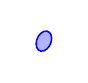
\begin{tikzpicture}[scale=.06]
    \begin{axis}
    [xmin=0, xmax=5,
    ymin=0, ymax=5,
    axis line style = {draw=none},
    ticks=none]
    	\draw[blue, line width=9pt, fill=blue,fill opacity=0.3] \pgfextra{
    	  \pgfpathellipse{\pgfplotspointaxisxy{2.5}{2.5}}
    		{\pgfplotspointaxisdirectionxy{0}{1.8}}
        	{\pgfplotspointaxisdirectionxy{1.2}{.5}}
    	};
    \end{axis}
    \end{tikzpicture}
    }
    \frac{\alpha_s}{\pi}~
    \frac{\dd\theta}{\theta}~
    \dd z~
    [\bar{p}_i(z)]^{(1/2)}_+
    ~~~
    \triangleq
    ~~~
    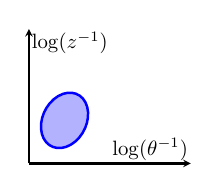
\begin{tikzpicture}[
    baseline={([yshift=-.8ex]current bounding box.center)},
    vertex/.style={anchor=base,
    circle,fill=black!25,minimum size=18pt,inner sep=2pt},
    scale=.3]
    \begin{axis}
    [
    xlabel=\scalebox{2.5}
    {\(\log(\theta^{-1})\)},
    ylabel=\scalebox{2.5}
    {\(\log(z^{-1})\)},
    xmin=0, xmax=5,
    ymin=0, ymax=5,
    axis line style = {line width=3pt},
    axis y line*=left,
    axis x line*=bottom,
    axis lines = middle,
    ticks=none]
    	\draw[blue, line width=3pt, fill=blue,fill opacity=0.3]
    	\pgfextra{
    	  \pgfpathellipse{\pgfplotspointaxisxy{1.1}{1.6}}
    		{\pgfplotspointaxisdirectionxy{-.2}{.9}}
    		{\pgfplotspointaxisdirectionxy{.7}{.5}}
    	};
    \end{axis}
    \end{tikzpicture}
    ~~~
    \triangleq
    ~~~
    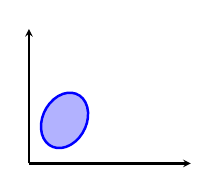
\begin{tikzpicture}[
    baseline={([yshift=-.8ex]current bounding box.center)},
    vertex/.style={anchor=base,
    circle,fill=black!25,minimum size=18pt,inner sep=2pt},
    scale=.3]
    \begin{axis}
    [xmin=0, xmax=5,
    ymin=0, ymax=5,
    axis line style = {line width=3pt},
    axis y line*=left,
    axis x line*=bottom,
    axis lines = middle,
    ticks=none]
    	\draw[blue, line width=3pt, fill=blue,fill opacity=0.3]
    	\pgfextra{
    	  \pgfpathellipse{\pgfplotspointaxisxy{1.1}{1.6}}
    		{\pgfplotspointaxisdirectionxy{-.2}{.9}}
    		{\pgfplotspointaxisdirectionxy{.7}{.5}}
    	};
    \end{axis}
    \end{tikzpicture}
    ,
\end{align}
where the shaded oval in the Lund plane above represents an arbitrary shape associated with a region of two-particle phase space.
\end{definitionbox}


\remark{}{
It follows, for example, that
%
\begin{align}
    \label{eq:plus-fn-diagram-identities}
    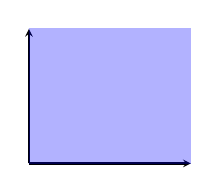
\begin{tikzpicture}[
    baseline={([yshift=-.8ex]current bounding box.center)},
    vertex/.style={anchor=base,
    circle,fill=black!25,minimum size=18pt,inner sep=2pt},
    scale=.3]
    \begin{axis}
    [xmin=0, xmax=5,
    ymin=0, ymax=5,
    axis line style = {line width=3pt},
    axis y line*=left,
    axis x line*=bottom,
    axis lines = middle,
    ticks=none]
    	\draw[blue, line width=3pt, fill=blue,fill opacity=0.3]
    	\pgfextra{
    	  \pgfpathellipse{\pgfplotspointaxisxy{0}{0}}
    		{\pgfplotspointaxisdirectionxy{0}{100}}
    		{\pgfplotspointaxisdirectionxy{100}{0}}
    	};
    \end{axis}
    \end{tikzpicture}
    =
    0
    ~~~~~~~~~
    {\rm and}
    ~~~~~~~~~
    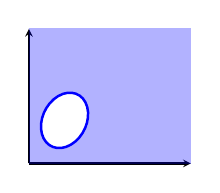
\begin{tikzpicture}[
    baseline={([yshift=-.8ex]current bounding box.center)},
    vertex/.style={anchor=base,
    circle,fill=black!25,minimum size=18pt,inner sep=2pt},
    scale=.3]
    \begin{axis}
    [xmin=0, xmax=5,
    ymin=0, ymax=5,
    axis line style = {line width=3pt},
    axis y line*=left,
    axis x line*=bottom,
    axis lines = middle,
    ticks=none]
    	\draw[blue, line width=3pt, fill=blue,fill opacity=0.3]
    	\pgfextra{
    	  \pgfpathellipse{\pgfplotspointaxisxy{0}{0}}
    		{\pgfplotspointaxisdirectionxy{0}{100}}
    		{\pgfplotspointaxisdirectionxy{100}{0}}
    	};
    	\draw[blue, line width=3pt, fill=white,fill opacity=1.0]
    	\pgfextra{
    	  \pgfpathellipse{\pgfplotspointaxisxy{1.1}{1.6}}
    		{\pgfplotspointaxisdirectionxy{-.2}{.9}}
    		{\pgfplotspointaxisdirectionxy{.7}{.5}}
    	};
    \end{axis}
    \end{tikzpicture}
    ~~
    =
    ~~
    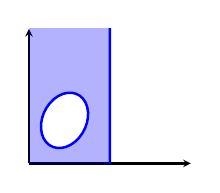
\begin{tikzpicture}[
    baseline={([yshift=-.8ex]current bounding box.center)},
    vertex/.style={anchor=base,
    circle,fill=black!25,minimum size=18pt,inner sep=2pt},
    scale=.3]
    \begin{axis}
    [xmin=0, xmax=5,
    ymin=0, ymax=5,
    axis line style = {line width=3pt},
    axis y line*=left,
    axis x line*=bottom,
    axis lines = middle,
    ticks=none]
    	\draw[blue, line width=3pt, fill=blue,fill opacity=0.3]
    	\pgfextra{
    	  \pgfpathellipse{\pgfplotspointaxisxy{0}{.9}}
    		{\pgfplotspointaxisdirectionxy{0}{200}}
    		{\pgfplotspointaxisdirectionxy{2.5}{.9}}
    	};
    	\draw[blue, line width=3pt, fill=white,fill opacity=1.0]
    	\pgfextra{
    	  \pgfpathellipse{\pgfplotspointaxisxy{1.1}{1.6}}
    		{\pgfplotspointaxisdirectionxy{-.2}{.9}}
    		{\pgfplotspointaxisdirectionxy{.7}{.5}}
    	};
    \end{axis}
    \end{tikzpicture}
    ~~
    =
    ~~
    -~
    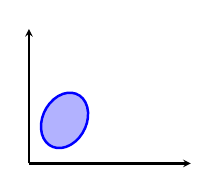
\begin{tikzpicture}[
    baseline={([yshift=-.8ex]current bounding box.center)},
    vertex/.style={anchor=base,
    circle,fill=black!25,minimum size=18pt,inner sep=2pt},
    scale=.3]
    \begin{axis}
    [xmin=0, xmax=5,
    ymin=0, ymax=5,
    axis line style = {line width=3pt},
    axis y line*=left,
    axis x line*=bottom,
    axis lines = middle,
    ticks=none]
    	\draw[blue, line width=3pt, fill=blue,fill opacity=0.3]
    	\pgfextra{
    	  \pgfpathellipse{\pgfplotspointaxisxy{1.1}{1.6}}
    		{\pgfplotspointaxisdirectionxy{-.2}{.9}}
    		{\pgfplotspointaxisdirectionxy{.7}{.5}}
    	};
    \end{axis}
    \end{tikzpicture}
    .
\end{align}
As depicted above, we may replace any vertical line -- representing an integral over \(z\) at fixed \(\theta\) -- or any vertical strip -- representing an integral over \(z\) and some range of \(\theta\) -- with zero, since the integral of a \gls{plus-fn} is zero.
}



\begin{example}
    \label{ex:mass-fixed-order}
    The pairwise mass of two massless partons emerging from a single splitting is given by
    \begin{equation}
    \begin{aligned}
        m^2 &= (p_1 + p_2)^2 = 2 p_1 \cdot p_2
        =
        2 Q^2
        \,
        z \, (1-z)
        \le(1 - \cos(\theta)\ri)
        \\
        &\approx
        Q^2 z \theta^2
        .
    \end{aligned}
    \end{equation}

    The corresponding \gls{substructure-diagram} showing the veto region \(z\theta^2 > m^2 / Q^2\) is
    \begin{center}
    \begin{tikzpicture}[scale=0.5]
    \begin{axis}
    [xlabel=\(\log(\theta^{-1})\), ylabel=\(\log(z^{-1})\),
    xmin=0, xmax=5,
    ymin=0, ymax=5,
    axis line style = very thick,
    axis y line*=left,
    axis x line*=bottom,
    axis lines = middle,
    ticks=none]
        \addplot[name path=f,domain=0:5,
        style=very thick,blue]
        {4.5-1.5*x};

        \path[name path=axis]
        (axis cs:0,0) -- (axis cs:1,0);

        \addplot [
            thick,
            color=blue,
            fill=blue,
            fill opacity=0.3
        ]
        fill between[
            of=f and axis
        ];

        \node [rotate=-50] at (axis cs:  2.2,  2.3) {$m^2 = z\theta^2$};
    \end{axis}
    \end{tikzpicture}
    \end{center}

    We can easily read off the resummed distribution for the mass squared of a jet at the level of accuracy we are pursuing (leaving the integrals to you):
    \begin{align}
        \Sigma(m^2)
        \approx
        -
        \,\,\,
        \raisebox{-10pt}{
        \begin{tikzpicture}[
        baseline={([yshift=-.8ex]current bounding box.center)},
        vertex/.style={anchor=base,
        circle,fill=black!25,minimum size=18pt,inner sep=2pt},
        scale=.3]
        \begin{axis}
        [xmin=0, xmax=5,
        ymin=0, ymax=5,
        axis line style = very thick,
        axis y line*=left,
        axis x line*=bottom,
        axis lines = middle,
        ticks=none]
        	\addplot[name path=f,domain=0:5,
            style=very thick,blue]
            {4.5-1.5*x};
            \path[name path=axis]
            (axis cs:0,0) -- (axis cs:1,0);
            \addplot [
                thick,
                color=blue,
                fill=blue,
                fill opacity=0.3
            ]
            fill between[
                of=f and axis
            ];
        \end{axis}
        \end{tikzpicture}
        }
        =
        -
        \frac{\alpha_{\rm S}}{\pi}
        \iint_{z\theta^2 > m^2}
        \dd\log(\theta) ~~ \dd z ~ [p(z)]_+
    \end{align}

    Plugging in the leading, singular piece for the splitting function at leading logarithmic accuracy, \(p(z) \sim 2 C_R / z\) for a splitting initiated by a parton with \(SU(3)\) color representation \(R\), and putting back in factors of \(Q\), we find
    \begin{align}
        \Sigma(m^2)
        \approx
        -\frac{C_R\alpha_{\rm S}}{2 \pi}\log^2\left(\frac{m^2}{Q^2}\right)
        \,,
    \end{align}
    with the associated pseudo-probability density
    \begin{align}
        \rho(m^2)
        =
        \frac{\dd}{\dd m^2} \Sigma(m^2)
        \approx
        \frac{C_R \alpha_s}{\pi}
        \frac{1}{m^2}
        \log\le(\frac{Q^2}{m^2}\ri)
        \,.
    \end{align}

    This describes the mass-squared distribution for a two-particle final state in the collinear limit.
    %
    We will include the effects of many emissions in \Sec{ll-substructure-diagrams} of \Chap{jets}.
\end{example}
~\\

\begin{exercise}{}
    Repeat the analysis of Example \ref{ex:mass-fixed-order} above with and without \glspl{substructure-diagram} for the leading pieces of the NLO distributions of \glspl{angularity} \(e_\varsigma\) (\Eq{angularitydefn_lo}) and \glspl{gecf} \(C_1^{(\varsigma)}\) (\Eq{GECFdefn_lo}).
    %
    I find
    \begin{subequations}
    \begin{align}
        \Sigma_{\le(e_\varsigma\ri)}(x)
        \approx
        \Sigma_{\le(C_1^{(\varsigma)}\ri)}(x)
        \,\,
        &\approx
        \,\,
        -\frac{C_R\alpha_{\rm S}}{\varsigma \pi}\log^2(x)
        \\
        \rho_{\le(e_\varsigma\ri)}(x)
        \approx
        \rho_{\le(C_1^{(\varsigma)}\ri)}(x)
        \,\,
        &\approx
        \,\,
        -\frac{C_R\alpha_{\rm S}}{\varsigma \pi} \frac{1}{x}
        \log\left(x\right)
        \,.
    \end{align}
    \end{subequations}
    Compare these to the results obtained above for the mass distribution.
\end{exercise}



% ---------------------------------------
\subsection{Eikonal Gluons are Angular-Ordered}
% ---------------------------------------
\label{sec:eikonal-limit}

The factorization formulae of this section all hold in the \textit{eikonal limit}, which for our purposes describes the physics of particles which are very low-energy or very collinear:

\begin{definitionbox}{Eikonal Limit}{eikonal-limit}
    In \gls{qft}, the \vocab{eikonal limit} refers to a limit in which the four-momenta of two particles become nearly collinear.
    %
    More precisely, the \vocab{eikonal limit for particles \(i\) and \(j\)} is associated with the region of phase space in which the pair of particles \(i\) and \(j\) are far more collinear than any other pair of particles in a scattering event:
    \begin{align}
        \label{eq:eikonal-limit}
        p_i \cdot p_j \ll p_\ell \cdot p_m\qquad \forall \,\, \ell, m
        \,.
    \end{align}
\end{definitionbox}


\remark{}{
    The eikonal limit for massless particles \(i\) and \(j\) implies that either \(i\) and \(j\) are very collinear or that at least one is very low energy.
    %
    In particular, setting \(i = \ell\) in \Eq{eikonal-limit} and using massless particles, for which \(
        p_i \cdot p_j
        =
        E_i E_j \le(1 - \hat{n}_i \cdot \hat{n}_j\ri)
    \),
    %
    we have
    \begin{align}
        E_j \le(1 - \hat{n}_i \cdot \hat{n}_j\ri)
        \ll
        E_k \le(1 - \hat{n}_i \cdot \hat{n}_k\ri)
        \,,
    \end{align}
    for all \(k\).
    %
    If we write \(1-\hat{n}_\ell \cdot \hat{n}_m \approx \theta^2_{\ell m}/2\), we can conclude that for all \(k\),
    \begin{align}
        E_j \theta^2_{ij}
        \ll
        E_k \theta^2_{ik}
        \,,
    \end{align}
    and similarly when \(i\) and \(j\) are flipped.
    %
    If \(E_j\) and \(E_k\) are of similar magnitude, \(E_j \sim E_k\), then \(\theta^2_{ij} \ll \theta^2_{ik}\);
    %
    otherwise, if \(\theta^2_{ij} \sim \theta^2_{ik}\), then \(E_j \ll E_k\).
    %
    Therefore, either \(\theta^2_{ij} \ll \theta^2_{ik}, \theta^2_{jk}\) or \(E_i, E_j \ll E_k\), for all \(k\).
}



Closely related is the \textit{soft limit} involving only a single particle:
\begin{definitionbox}{Soft Limit}{soft-limit}
    The \vocab{soft limit} for a particle with momentum \(q\) is the limit in which the particle is eikonal with respect to any \textit{other} particle/pair of particles in the scattering event:
    \begin{align}
        q \cdot p_i \ll p_j \cdot p_k \qquad \forall\,i,j,k
        \,,
    \end{align}
    where the \(p_j\) and \(p_k\) do not include \(q\).
    %
    In what follows in this section, we also say that the particle with momentum \(q\) is \vocab{soft}.
\end{definitionbox}


The eikonal limit was originally used as a tool in geometric optics (hence the name, from the Greek \(\varepsilon \acute{\iota}\kappa \acute{\omega}\nu\), meaning `image'' and the root of the more common English word ``icon'').
%
Once light was discovered to be a wave, the eikonal limit was taken from optics and applied to the more general mechanics of waves.
%
Today, it is in the description of waves in electromagnetism, non-relativistic quantum mechanics, and our current context:
%
particle physics and quantum field theory.

In \gls{qft} the eikonal limit describes universal features of the radiation accompanying charged matter;
%
roughly, it captures features of the cloud of photons corresponding to the electric field surrounding an electron, and the cloud of gluons accompanying quarks.
%
Due to the universality of eikonal radiation, the amplitudes describing scattering in gauge theories -- including electrodynamics, \gls{qcd}, the \gls{sm}, and even gravity -- take a remarkably simple form.

An early an extremely powerful result demonstrating the universality of eikonal physics in \gls{qft} was found by Low in the study of QED \cite{}.
%
In the language that will be useful for our purposes, we may write

\begin{theorembox}{Soft Photon Theorem (Low \cite{})}{soft-photon}
    Consider an \(N\)-particle, on-shell amplitude \(\mathcal{M}(p_1, \cdots, p_{N-1};\,q,\,\epsilon)\) in which \(q\) and \(\epsilon\) are the momentum and polarization four-vector of a \vocab{soft photon}.
    %
    In this limit, the amplitude can be factorized in terms of \vocab{eikonal factors} and \(N-1\)-particle, \textit{off-shell} amplitudes:
    \begin{equation}
    \begin{aligned}
        \mathcal{M}_N
        &=
        \sum_{i}
        Q_i
        \,
        (-1)^{\eta_i}
        \,
        \frac{\epsilon \cdot p_i}{p_i \cdot q}
        \widehat{\mathcal{M}}_{N-1,\,(i)}
        \quad
        +
        \quad
        \mathcal{O}\le(\frac{q\cdot p}{p \cdot p}\ri)
        \,,
    \end{aligned}
    \end{equation}
where \(\mathcal{M}_N\) indicates the on-shell amplitude, while \(\widehat{\mathcal{M}}_{N-1,\,(i)}\) indicates the off-shell amplitude in which the soft photon and particle \(i\) are merged,
    \begin{align}
        \mathcal{M}_N
        &:=
        \mathcal{M}_N(p_1,\,\cdots,\,\,p_{N-1};\,q,\,\epsilon)
        \,,
        \\
        \widehat{\mathcal{M}}_{N-1,\,(i)}
        &:=
        \mathcal{M}_{N-1}(
            p_1,\,\cdots,\,
            p_{i-1},\,
            p_i + q,\,
            p_{i+1},\,
            \cdots,\,\,p_{N-1}
        )
        \,,
    \end{align}
    \(Q_i\) indicates the electromagnetic charge of particle \(i\), \(\eta_i\) is 0 if particle \(i\) is incoming and 1 if it is outgoing, and the corrections are suppressed in the soft limit.
    %
    We have suppressed the spin labels of the additional particles (i.e. the particles with momenta \(p_i\)), but they remain unchanged between \(\mathcal{M}_N\) and \(\mathcal{M}_{N-1}\).
    %
    \sam{Right?}
\end{theorembox}

Notably, by expanding \(\widehat{\mathcal{M}}_{N-1}\) in powers of \(q\), it can be approximated as an on-shell amplitude up to terms which can be neglected in the soft limit.


\begin{exercise}
    Using Low's soft photon theorem, argue that gauge invariance of the amplitude \(\mathcal{M}_N\) implies the conservation of charge.

    \vspace{7pt}
    \hrule
    \vspace{7pt}

    \texttt{(Hint:)}
    %
    Use the common trick that gauge invariance implies that \(q^\mu \mathcal{R}_\mu = 0\), where \(\mathcal{R}^\mu\) is the polarization-stripped amplitude (or ``remainder'') associated with the amplitude \(\mathcal{M}\) but with the polarization of the photon with momentum \(q\) removed.
    %
    % Actually, both \(q_\mu \mathcal{R}^\mu = 0\) and the soft photon theorem itself can be derived by using \textit{Ward-Takahashi} identities associated with gauge invariance.
\end{exercise}

\begin{exercise}
    \label{ex:soft-eikonal-photon}
    Using Low's theorem, argue that in the soft limit in which a photon is \textit{also} fully eikonal with a particle \(p_i\), the amplitude for the emission of a soft-eikonal photon can be written as a single factorized term (i.e. with no summation).
\end{exercise}


\remark{}{
    Low-Burnett-Kroll Theorem \cite{}, subleading soft theorem.
    %
    \sam{complete}
    %
    A modern presentation, and a note of the failure of the theorem to describe loop-level amplitudes, in \Reff{}.
    % https://arxiv.org/pdf/1412.3108
}


\begin{example}
    \label{ex:qed-antennae}
    In calculating scattering amplitudes, we will be interested in the \textit{squares} of amplitudes.
    %
    The polarization-averaged square of the amplitude given in the soft photon theorem has a satisfyingly simple form.
    %
    For the moment, let us assume that all charged particles are outgoing.%
    \footnote{
        We are interested in jets in this thesis, which are a final-state radiation phenomenon, and the appropriate factors of \((-1)^{\eta_i}\) can be put back in as necessary.
    }
    %
    Then, ignoring \(\mathcal{O}(q)\) corrections so that we may take \(\widehat{\mathcal{M}}_{N-1,\,(i)} \to \mathcal{M}_{N-1}\) to be on-shell, the squared \(N\)-particle amplitude takes the factorized form
    \begin{align}
        \abs{\mathcal{M}_N}^2
        =
        \epsilon^{\mu} \epsilon^{*\nu}
        \abs{\mathcal{M}_{N-1}}^2
        \sum_{i,\,j}
        Q_i Q_j
        \frac{p_i^\mu p_j^\nu}
            {\le(p_i\cdot q\ri)\le(p_j \cdot q\ri)}
        \,.
    \end{align}

    By performing a sum on the polarizations of the soft photon, we have
    \begin{align}
        \sum_{\epsilon}
        \abs{\mathcal{M}_N}^2
        &=
        \abs{\mathcal{M}_{N-1}}^2
        \sum_{i,\,j}
        Q_i Q_j
        \frac{p_i \cdot p_j}
            {\le(p_i\cdot q\ri)\le(p_j \cdot q\ri)}
        % \\
        % &=
        % \abs{\mathcal{M}_{N-1}}^2
        % \sum_{i,\,j}
        % Q_i Q_j
        % \frac{p_i \cdot p_j}{\le(p_i + p_j\ri)\cdot q}
        % \le(
        %     \frac{1}{p_i \cdot q} + \frac{1}{p_j\cdot q}
        % \ri)
        \,.
    \end{align}
    %where the final equality follows by a simple algebraic manipulation.
    %%
    %\begin{align}
    %    \sum_{\epsilon}
    %    \abs{\mathcal{M}_N}^2
    %    &=
    %    \abs{\mathcal{M}_{N-1}}^2
    %    \times
    %    2
    %    \sum_i
    %    \frac{1}{p_i \cdot q}
    %    \sum_j
    %    Q_i Q_j
    %    \frac{p_i \cdot p_j}{\le(p_i + p_j\ri)\cdot q}
    %    \,.
    %\end{align}
    %Due to the factor of \(1/p_i\cdot q\), the first summed particle labelled \(i\) is sometimes called the \textit{emitter};
    %%
    %the second particle, labelled \(j\), is sometimes called the \textit{spectator}, and accounts for some subtle features of momentum recoil and, in \gls{qcd}, additional color correlations \cite{}.

    The additional factor \(A_{ij} = Q_i Q_j p_i \cdot p_j / (p_i \cdot q) (p_j \cdot q)\) is sometimes called the \vocab{antenna pattern} or the \vocab{antenna factor} for the pair \((ij)\).
\end{example}


When applied to the gluonic radiation of \gls{qcd}, the principles that led to the soft photon theorem lead to the more complicated \glslink{eikonal}{\textit{soft gluon theorem}}:
\begin{theorembox}{Soft Gluon Theorem}{soft-gluon}
    Consider an \(N\)-particle, on-shell amplitude \(\mathcal{M}_N\le(p_1,\,r_1; \cdots;\,p_{N-1},\,r_{N-1};\,q,\,a\,\epsilon\ri)\).
    %
    The \(p_i\) indicate external momenta.
    %
    The \(r_i\) indicate the color labels of the external particles (e.g. \(r_q \in \{\)red, blue, green\(\}\) for a quark, while \(r_g \in \{1,\cdots,N_c^2-1\}\) for a gluon).
    %
    \(q\), \(a\), and \(\epsilon\) indicate the momentum, color label, and polarization of a \vocab{soft gluon}, respectively.

    In the soft limit, this amplitude can be factorized in terms of eikonal factors and \(N-1\)-particle, off-shell amplitudes as:
    \begin{equation}
    \begin{aligned}
        \mathcal{M}^{(r_1\cdots r_{N-1}\,a)}_N
        &=
        \sum_{i}
        g_s
        \le(T^a_{R_i}\ri)\indices{^{\eta_i}_{r_i\,r'_i}}
        \,
        \frac{\epsilon \cdot p_i}{p_i \cdot q}
        \widehat{\mathcal{M}}
        ^{(r_1\cdots r'_i\cdots r_{N-1})}
        _{N-1,\,(i)}
        \quad
        +
        \quad
        \mathcal{O}\le(\frac{q\cdot p}{p \cdot p}\ri)
        \,,
    \end{aligned}
    \end{equation}
    where now the superscripts for \(\mathcal{M}_N\) and \(\widehat{\mathcal{M}}_{N-1}\) denote the color labels of the associated external particles, \(T_{R_i}\) indicates the generator of the gauge group in the representation \(R_i\) associated with particle \(i\), and \(\eta_i\) indicates the complex conjugate representation if particle \(i\) is outgoing.
    %
    As before, however, \(\widehat{\mathcal{M}}_{N-1}\) is approximately on-shell to leading order in \(q\).
\end{theorembox}

\remark{}{
    I have been unable to find the first presentation of the soft gluon theorem as a non-Abelian extension of Low's soft photon theorem.
    %
    The first direct proof sketch for the soft gluon theorem I have found is in \Reff{}.
    % https://arxiv.org/pdf/hep-ph/9605323
    %
    However, results involving eikonal gluon radiation appear earlier in the literature, even in textbooks \cite{}.
    %
    It may be that this result was known before an explicit proof was published.
}

\begin{exercise}
    Apply gauge invariance once again to obtain the manifestation of non-Abelian charge conservation for scattering amplitudes:
    \begin{align}
        \sum_{i}
        \le(T^a_{R_i}\ri)\indices{^{\eta_i}_{r_i\,r'_i}}
        \,
        \widehat{\mathcal{M}}
        ^{(r_1\cdots r'_i\cdots r_{N-1})}
        _{N-1,\,(i)}
        =
        0
        \,.
    \end{align}
\end{exercise}

\begin{exercise}
    In preparation for partonic scattering, the analogous calculation of Example \ref{ex:qed-antennae} with only outgoing particles where the soft photon is replaced by a soft gluon yields a polarization-summed result
    \begin{align}
        \hspace{-2pt}
        \sum_{\epsilon}
        \abs{\mathcal{M}_N^{(r_1\cdots r_{N-1}a)}}^2
        \!\!\!
        =
        \!
        \sum_{i, j}
        \frac{p_i \cdot p_j}
            {\le(p_i\cdot q\ri)\le(p_j \cdot q\ri)}
        \mathcal{M}_{N-1}^{(r_1\cdots r'_i \cdots r_{N-1})}
        \mathcal{M}_{N-1}^{(r_1\cdots r'_j \cdots r_{N-1})\,*}
        \!\!
        \le(T^a_{R_i}\ri)_{r_i r'_i}
        \le(T^a_{R_j}\ri)_{r'_j r_j}
        \!
        .
    \end{align}
    \sam{finish}
\end{exercise}


We now demonstrate a remarkable and important property of the antenna pattern for (spin-1) gauge theory amplitudes, such as the QED antenna pattern of \Example{qed-antennae}:
%
\sam{explanation in words}.
%
This property is referred to as \textit{angular ordering}, and is \textbf{essential} for the description of jets given in \Chap{jets}.


\begin{proposition}{Angular Ordering}{angular-ordering}
    \sam{complete}
\end{proposition}


\remark{}{
    \sam{Can replace the factor \(\dd \omega / \omega\) with \(p(z) \dd z\)}
}



% ==============================================
\section{Connecting back out}
% ==============================================

\sam{Test}


\begin{subappendices}



% If appendices to stand are their own
\iffalse
% %%%%%%%%%%%%%%%%%%%%%%%%%%%%%%%%%%%%
% Appendices
% %%%%%%%%%%%%%%%%%%%%%%%%%%%%%%%%%%%%
% \begin{subappendices}
% Chapter titles without numbers
\titleformat{\chapter}[display]
{\normalfont\huge\bfseries\sffamily}{}{0pt}{\chaptitlenonumber}

\titlespacing*{\chapter}{0pt}{0pt}{0pt}
% Chapter title
\clearpage
\chapter*{\hspace{-30pt}Appendix: QCD Compendium}
% TODO: chapter 2 appendix formatting
% phantomsection for use with hyperref, comment otherwise
\phantomsection
%
\addcontentsline{toc}{chapter}
    {\bf\\Appendix for Chapter 2: QCD Compendium}

\counterwithin{figure}{section}
\counterwithin{table}{section}
% Chapter titles with numbers
\titleformat{\chapter}[display]
{\normalfont\huge\bfseries\sffamily}{}{25pt}{\chaptitle}
\titlespacing*{\chapter} {0pt}{110pt}{20pt}


% % ===========================================================
% \section{Feynman Rules and Representation Theory}
% % ===========================================================

\begin{itemize}
    \item
        \sam{Change title? More about QCD...}

    \item
        Discussion of SU(3) and SU(N)

    \item
        Discussion of approximate and exact symmetries

    \item
        More on flavor, tabulation of quark masses, discussion of active flavors (see textbook for nice discussions)

    \item
        Birdtracks?
\end{itemize}

\fi


% ---------------------------------------
% \Soln{QCD at Loop Level}{qcd-loop}
% ---------------------------------------

\section{A QCD Compendium}
\label{app:qcd-compendum}

\iffalse
In order to perform perturbative renormalization, let's first introduce the real-space action in terms of renormalized fields:
\begin{subequations}
\begin{align}
	\mathcal{L}
    &=
    -\frac{1}{4}
    Z_A^2
    F\indices{^a_{\mu\nu}} F\indices{^{a\,\mu\nu}}
    +
    \sum_\text{flavors}
        Z_q^2
        \,\,
        \bar{q}_j
        \le(
            i \slashed{D}\indices{^j_i}
            -
            m Z_m \delta\indices{^j_i}
        \ri)
        q^i
    \,,
\end{align}
\sam{expand out D slash, move definition to main text}

\begin{align}
    \le(D_\mu\ri)_{ij}
    =
    \delta\indices{^j_i} \partial_\mu
    +
    i g \le(T_F^a A\indices{^a_{\mu}}\ri)\indices{^j_i}
    \,.
\end{align}


i.e. with the bare fields and couplings given by
\begin{align}
    \sqrt{Z_q}\,q_i &= q_{(0)}
    \,,
    \qquad
    \sqrt{Z_A}\,A\indices{^a_\mu} = A\indices{^a_{\mu\,\,(0)}}
    \,,
    \qquad
    \\
    \frac{\mu^{\epsilon}\,Z_g}{\sqrt{Z_A} \, Z_q} \,\, g &
    = g_{(0)}
    \,,\qquad\quad
    % \frac{\mu^{2\epsilon}\,Z_\lambda}{Z_\phi^2}
    \mu^{\sam{???}}
    Z_q^2 \, Z_m \, m = m_{(0)}
    % \,,\qquad\quad
    % \frac{\mu^{2\epsilon}\,Z_\lambda}{Z_\phi^2}
    % \lambda = \lambda_{(0)}
    \label{eq:bare_coupling}
    \,.
\end{align}
\end{subequations}
\fi

\begin{answer}
\begin{center}
{\normalfont\Large\bfseries\sffamily The Rules for the Gluon Sector of QCD are:}
\end{center}

\begin{subequations}
\begin{align}
\raisebox{0pt}{
\begin{tikzpicture}
    \begin{feynman}
        % vertices
        \vertex (i) at (-1.5,0.0);
        \vertex (f) at (1.5,0.0);
        % edge labels
        \vertex [above left=-0.8pt and 0.0ptof i] (ti) {$a, \mu$};
        \vertex [above right=0.0pt and 0.0pt of f] (tf) {$b,\nu$};
        % diagram
        \diagram* {
            (i)
            -- [gluon, momentum=\(p\)]
            (f)
            ,
        };
    \end{feynman}
\end{tikzpicture}
}
\quad
:=
\quad
&
i\, \delta^{ab} \frac{-g_{\mu\nu} + (1-\xi) p_\mu p_\nu / p^2}{p^2 + i 0^+}
\\
\notag
\quad
\xrightarrow[\text{Feynman gauge}]{}
\quad
&
\delta^{ab} \frac{-i g_{\mu\nu}}{p^2 + i 0^+}
\end{align}

\begin{align}
\raisebox{-40pt}{
\begin{tikzpicture}
    \begin{feynman}
        % vertices
        \vertex (u) at (0,1.5);
        \vertex (l) at (-1.30,-0.75);
        \vertex (r) at (1.30,-0.75);
        \vertex (cen) at (0,0);
        % edge labels
        \vertex [below left=-0.8pt and 0.0ptof l] (tl) {$a, \mu$};
        \vertex [above left=-0.8pt and 0.0ptof u] (tu) {$b, \nu$};
        \vertex [above right=0.0pt and 0.0pt of r] (tr) {$c,\rho$};
        % diagram
        \diagram* {
            (l)
            -- [gluon, momentum=\(p\)]
            (cen)
            ,
            (u)
            -- [gluon, momentum=\(q\)]
            (cen)
            ,
            (r)
            -- [gluon, momentum=\(r\)]
            (cen)
        };
    \end{feynman}
\end{tikzpicture}
}
\quad
:=
\quad
-g f^{abc} \le[
    \begin{array}{rrr}
    (q-r)_\mu
    &
    g_{\nu\rho}
    &
    \\
    +&&
    \\
    (r-p)_\nu
    &
    g_{\rho\mu}
    &
    \\
    +&&
    \\
    (p-q)_\rho
    &
    g_{\mu\nu}
    &
    \end{array}
\ri]
\,.
\end{align}

\begin{align}
\raisebox{-40pt}{
\begin{tikzpicture}
    \begin{feynman}
        % vertices
        \vertex (ul) at (-1.0,1.0);
        \vertex (ll) at (-1.0,-1.0);
        \vertex (ur) at (1.0,1.0);
        \vertex (lr) at (1.0,-1.0);
        \vertex (cen) at (0,0);
        % edge labels
        \vertex [above left=-0.8pt and 0.0ptof ul] (tu) {$a, \mu$};
        \vertex [above left=-0.8pt and 0.0ptof ll] (tl) {$b, \nu$};
        \vertex [above right=0.0pt and 0.0pt of ur] (tr) {$c,\rho$};
        \vertex [above right=0.0pt and 0.0pt of lr] (tr) {$d,\sigma$};
        % diagram
        \diagram*{
            (ul)
            -- [gluon]
            (cen)
            ,
            (ur)
            -- [gluon]
            (cen)
            ,
            (ll)
            -- [gluon]
            (cen)
            ,
            (lr)
            -- [gluon]
            (cen)
        };
    \end{feynman}
\end{tikzpicture}
}
\quad
:=
\quad
&
-i g^2
\le[
\begin{array}{rrr}
    & f^{\bar{e}ac} f^{\bar{e}bd} &\le(g_{\mu\nu} g_{\rho\sigma} - g_{\mu\sigma} g_{\nu\rho}\ri)
    \\
    +& f^{\bar{e}ad} f^{\bar{e}bc} &\le(g_{\mu\nu} g_{\rho\sigma} - g_{\mu\rho} g_{\nu\sigma}\ri)
    \\
    +& f^{\bar{e}ab} f^{\bar{e}cd} &\le(g_{\mu\rho} g_{\nu\sigma} - g_{\mu\sigma} g_{\nu\rho}\ri)
\end{array}
\ri]
\,,
\end{align}
where the ``barred'' index \(\bar{e}\) is marked only to indicate that it is summed over.

\end{subequations}
with the counterterm diagrams
\begin{subequations}
% \input{}
\end{subequations}
\end{answer}

\begin{answer}
\begin{center}
{\normalfont\Large\bfseries\sffamily The Rules for the Quark Sector of QCD are:}
\end{center}

\begin{subequations}
\begin{align}
\raisebox{0pt}{
\begin{tikzpicture}
    \begin{feynman}
        % vertices
        \vertex (i) at (-1.5,0.0);
        \vertex (f) at (1.5,0.0);
        % edge labels
        \vertex [above left=-0.8pt and 0.0ptof i] (ti) {$i$};
        \vertex [above right=0.0pt and 0.0pt of f] (tf) {$j$};
        % diagram
        \diagram* {
            (i)
            -- [fermion, momentum=\(p\)]
            (f)
            ,
        };
    \end{feynman}
\end{tikzpicture}
}
\quad
:=
\quad
&
i\, \delta\indices{^j_i} \frac{\slashed{p} + m}{p^2 - m^2 + i 0^+}
\end{align}

\begin{align}
\raisebox{-40pt}{
\begin{tikzpicture}
    \begin{feynman}
        % vertices
        \vertex (u) at (0,1.5);
        \vertex (l) at (-1.30,-0.75);
        \vertex (r) at (1.30,-0.75);
        \vertex (cen) at (0,0);
        % edge labels
        \vertex [above right=-0.8pt and 0.0ptof u] (tu) {$a, \mu$};
        \vertex [below left=-0.8pt and 0.0ptof l] (tl) {$i$};
        \vertex [below right=0.0pt and 0.0pt of r] (tr) {$j$};
        % diagram
        \diagram* {
            (cen)
            -- [gluon]%, momentum'=\(q\)]
            (u)
            ,
            (l)
            -- [fermion]%, momentum=\(p\)]
            (cen)
            ,
            (cen)
            -- [fermion]%, momentum=\(p-q\)]
            (r)
        };
    \end{feynman}
\end{tikzpicture}
}
\quad
:=
\quad
-i g \le(T^a\ri)\indices{^j_i}
\gamma^\mu
\,.
\end{align}

\end{subequations}
with the counterterm diagrams
\begin{subequations}
% \input{}
\end{subequations}
Let's also not forget that any time we have a closed fermion loop, the associated diagram gets an additional factor of \(-1\).
\end{answer}

\begin{answer}
\begin{center}
{\normalfont\Large\bfseries\sffamily The Rules for the Ghost Sector of QCD are:}

(in covariant gauges)
\end{center}

\begin{subequations}
\begin{align}
\raisebox{0pt}{
\begin{tikzpicture}
    \begin{feynman}
        % vertices
        \vertex (i) at (-1.5,0.0);
        \vertex (f) at (1.5,0.0);
        % edge labels
        \vertex [above left=-0.8pt and 0.0ptof i] (ti) {$a$};
        \vertex [above right=0.0pt and 0.0pt of f] (tf) {$b$};
        % diagram
        \diagram* {
            (i)
            -- [dotted, ultra thick, momentum=\(p\)]
            (f)
            ,
        };
    \end{feynman}
\end{tikzpicture}
}
\quad
:=
\quad
&
\delta^{ab} \frac{i}{p^2 + i 0^+}
\end{align}

\begin{align}
\raisebox{-40pt}{
\begin{tikzpicture}
    \begin{feynman}
        % vertices
        \vertex (u) at (0,1.5);
        \vertex (il) at (-0.65,-0.375);
        \vertex (l) at (-1.30,-0.75);
        \vertex (ir) at (0.65,-0.375);
        \vertex (r) at (1.30,-0.75);
        \vertex (cen) at (0,0);
        % edge labels
        \vertex [above right=-0.8pt and 0.0ptof u] (tu) {$a, \mu$};
        \vertex [below left=-0.8pt and 0.0ptof l] (tl) {$b$};
        \vertex [below right=0.0pt and 0.0pt of r] (tr) {$c$};
        % diagram
        \diagram* {
            (cen)
            -- [gluon]%, momentum'=\(q\)]
            (u)
            ,
            (l)
            -- [dotted, arrow, ultra thick]
            (il)
            -- [dotted, ultra thick]
            (cen)
            ,
            (cen) -- [dotted, ultra thick, momentum=\(r\)] (r)
            ,
            (cen)
            -- [dotted, arrow, ultra thick]
            (ir)
            -- [dotted, ultra thick]
            (r)
            ,
        };
    \end{feynman}
\end{tikzpicture}
}
\quad
:=
\quad
g f^{abc} r^\mu
\,.
\end{align}

\end{subequations}
with the counterterm diagrams
\begin{subequations}
% \input{}
\end{subequations}
\end{answer}


\vspace{20pt}
\hrule
\vspace{20pt}



\sam{Polarizations}
in Lorenz gauge, with \(\xi = 1\), polarization vectors take the form
%
so that they sum...

\sam{Spinor factors}
\sam{While results should be basis-independent, useful to use a chiral basis}
\begin{align}
    \gamma^\mu = \pmtrx{0 & \sigma^\mu\\\overline{\sigma}^\mu & 0}
    \,,
\end{align}
where \(\sigma^\mu = (1, \vec{\sigma})\) and \(\overline{\sigma}^\mu = (1, -\vec{\sigma})\) are invariant symbols of the Lorentz group.
%
In this basis, spinor factors take the form
\begin{align}
    u_s(p)
    &=
    \pmtrx{
        \sqrt{p\cdot \sigma}\ket{s}
        \\
        \sqrt{p\cdot{\overline{\sigma}}} \ket{s}
    }
    \\
    v_s(p)
    &=
    \pmtrx{
        \sqrt{p\cdot \sigma}\sigma_x \ket{s}
        \\
        -\sqrt{p\cdot{\overline{\sigma}}} \sigma_x \ket{s}
    }
    =:
    \pmtrx{
        \sqrt{p\cdot \sigma}\ket{\overline{s}}
        \\
        -\sqrt{p\cdot{\overline{\sigma}}} \ket{\overline{s}}
    }
    \,,
\end{align}
where we have abused notation by using \(\ket{s}\) to denote the 2-spinor encoding the particle's spin measured in the \(\sigma_z\)/computational basis.
%
For example,
\begin{align}
    \ket{s}
    =
    \begin{cases}
        \pmtrx{1\\0} & \text{spin } s \text{ is along } +\hat{z}
        \,,
        \\
        \pmtrx{0\\1} & \text{spin } s \text{ is along } -\hat{z}
        \,.
    \end{cases}
\end{align}
%
so that they sum...

At high energies, or in the massless limit, they reduce to
\begin{align}
    u_s(p)
    &=
    \sqrt{\frac{E}{2}}
    \pmtrx{
        \le(1 - \hat{p}\cdot \vec{\sigma}\ri)\ket{s}
        \\
        \le(1 + \hat{p}\cdot \vec{\sigma}\ri)\ket{s}
    }
    \\
    v_s(p)
    &=
    \sqrt{\frac{E}{2}}
    \pmtrx{
        \le(1 - \hat{p}\cdot \vec{\sigma}\ri) \ket{\overline{s}}
        \\
        -\le(1 + \hat{p}\cdot \vec{\sigma}\ri) \ket{\overline{s}}
    }
    \,,
\end{align}
so that
\begin{align}
    \sam{Other useful things?}
\end{align}



\vspace{20pt}
\hrule
\vspace{20pt}

\begin{subequations}
The \(T_F^a\) are usually represented in a standardized form in terms of the \vocab{Gell-Mann matrices} \(T_F^a \overset{\cdot}{=} \lambda^a/2\), with
\begin{gather}
    \lambda^1
    :=
    \pmtrx{0&1&0\\1&0&0\\0&0&0}
    \quad
    \lambda^2
    :=
    \pmtrx{0&-i&0\\i&0&0\\0&0&0}
    \quad
    \lambda^3
    :=
    \pmtrx{1&0&0\\0&-1&0\\0&0&0}
    \\
    \lambda^4
    :=
    \pmtrx{0&0&1\\0&0&0\\1&0&0}
    \quad
    \lambda^5
    :=
    \pmtrx{0&0&-i\\0&0&0\\i&0&0}
    \\
    \lambda^6
    :=
    \pmtrx{0&0&0\\0&0&1\\0&1&0}
    \quad
    \lambda^7
    :=
    \pmtrx{0&0&0\\0&0&-i\\0&i&0}
    \\
    \lambda^8
    :=
    \frac{1}{\sqrt{3}}
    \pmtrx{1&0&0\\0&1&0\\0&0&-2}
\end{gather}
\end{subequations}
with the normalization
\begin{subequations}
\begin{align}
    T_F = \frac{1}{2}
    \,.
\end{align}

\sam{?}
\begin{align}
    T_A = \frac{1}{2}
    \,.
\end{align}

\begin{align}
    C_F = \frac{2 N_c}{N_c^2 - 1}
    \to
    \frac{4}{3}
    \,.
\end{align}

\begin{align}
    C_A = N_c
    \to
    3
    \,.
\end{align}

In fact,
\begin{align}
    C_R = \frac{T_A C_A}{T_R}
    \,,
\end{align}
\sam{?}
which can be quickly and amusingly shown with \vocab{bird track diagrams} \cite{}.

\end{subequations}




% % ===========================================================
% \section{Splitting Functions}
% % ===========================================================

\begin{itemize}
    \item
        Splitting functions

    \item
        Moments

    \item
        Symmetrization subtleties

    \item
        Reduced splitting functions and subtleties
\end{itemize}


To begin, we provide explicit expressions for the DGLAP splitting functions, which describe the probability for the emission of partonic radiation from quarks and gluons, at one loop accuracy:
%
\begin{align}
&p_{q\to q g}(z) = C_F \frac{1+(1-z)^2}{z},
\label{eq:quark_splitting}
\\
&p_{g\to g g}(z) = 2C_A\frac{1-z}{z} + C_A z(1-z) + T_F n_f (z^2 + (1-z)^2).
\label{eq:gluon_splitting}
\end{align}
%
Here, \(z\) is the energy fraction of an emitted gluon relative to the total energy of the emitted gluon and an initial parton.
%
\(p_q\) describes the distribution of \(z\) in the case that a gluon emitted by a quark, \(q \to q g\), and \(p_g\) describes the distribution of \(z\) in the case \(g \to gg\).
%
\(T_F = \frac{1}{2}\) is the Dynkin index of the fundamental representation of the standard model SU(3) color gauge group, and \(n_f\) indicates the number of quark flavors.
%
In the following analysis, we take \(n_f = 5\), including all quark flavors except for the top quark.
%
As in the text, \(C_R\) is the quadratic Casimir for the representation \(R\) of SU(3).
%
\(C_R = C_F = \frac{4}{3}\) for quarks and \(C_R = C_A = 3\) for gluons.


% % ===========================================================
% \section{The Running Coupling}
% % ===========================================================

\begin{itemize}
    \item
        Not necessarily a useful appendix on its own, but helpful for explicit example of computation?

    \item
        Magnetic interpretation

    \item
        Short discussion of frozen coupling
\end{itemize}



% % ===========================================================
% \section{Event Shapes}
% % ===========================================================
% \begin{itemize}
%     \item
%         Definition, use cases

%     \item
%         Thrust (and historical use/connection)

%     \item
%         Thrust computation

%     \item
%         Connect to groomed event shapes

%     \item
%         Connect to EEC and EWOCs
% \end{itemize}



% Problems for Appendix
    % Problem about reduced splitting functions and moments?
    % \makeprob{}{}{
    % }

    % Problem about birdtracks and C(R) T(R) = C(A) T(A)?

    % Problem about f_abc f_abc?

    % Problem about universality of splitting functions by computing from different processes and matrix elements?

    % Derivation of thrust in e+e- collisions

    % Universal features of thrust from e+e- vs splitting functions?

\section{Distributions}
A generalized function (distribution) is defined through its action on test functions rather than pointwise values. It is useful for describing singularities and sharp transitions in physical models.

\begin{definitionbox}{Distribution}{distribution}
    \emph{\Glspl{distribution}} generalize the concept of functions to accommodate objects, like delta functions or \glslink{plus-fn}{plus-functions}, that do not correspond to traditional functions but can still be useful in the description of physical phenomena -- especially phenomena involving singularities.
    %
    Distributions can be understood in terms of their behavior when integrated against a space of test functions.

    \vspace{7pt}
    \hrule
    \vspace{7pt}

    More formally, a distribution \( T \) is a continuous linear functional that maps a test function \( \varphi(x) \) to a real or complex number.
    %
    By the \href{https://en.wikipedia.org/wiki/Riesz%E2%80%93Markov%E2%80%93Kakutani_representation_theorem}{\vocab{Riesz–Markov–Kakutani representation theorem}}, linear functionals are related to Borel measures on the space on which the corresponding functions act.
    %
    Thus, we may unambiguously write
    \[
    T[\varphi] = \int_{-\infty}^{\infty} T(x) \varphi(x) \, \dd x
    \]
    where \( \varphi(x) \) is a smooth test function.
\end{definitionbox}

A familiar example of a generalized function is the Dirac delta function, defined by
\begin{align}
    \delta(x-a)[\phi] = \int \delta(x-a)\phi(x) \dd x = \phi(a)
    \,.
\end{align}
%
Another useful distribution is the \vocab{Cauchy Principle Value}, which we examine in \Prob{principle-value}.


% --------------------------------------------------------
% Plus-function
% --------------------------------------------------------
The main reason we discuss distributions here, however, is the prominent role played by \glslink{plus-fn}{plus-functions} in this thesis in providing a concrete and consistent mathematical description of the singular behavior of partonic splitting.

% -----------------------------------
% Definition Comment:
% -----------------------------------
\begin{definitionbox}{
% Definition Header:
Plus-Distribution
}{}
    A \vocab{plus-distribution} (or ``plus-function'', or ``plus-function regulated distribution'') is a modified version of a ``parent function'' which is often so singular that it cannot be integrated on its own.
    %
    Plus-distribution regularization (or ``plus regularization'') turns the parent function into an integrable distribution.

    \vspace{7pt}
    \hrule
    \vspace{7pt}

    % Definition Body:
    Let us consider the following ingredients:
    \begin{itemize}
        \item
            let \(f(x)\) denote a function on \(\RR\);
        \item
            let \(\mc R \subset \RR\) denote a one-dimensional region;

        \item
            let \(p \in \mc R\) denote a point around which we would like \(f(x)\) to be regularized -- in most cases, \(f(x)\) will have a simple pole or similar singularity near \(p\).
    \end{itemize}

    The \vocab{plus-distribution} \(\le[f(x)\ri]_{+,p}^{x \in \mc R}\) is defined through its action on test functions in the integration region \(\mc R\):
    \begin{equation}
        \int_{\mc R} \dd x\le[f(x)\ri]_{+,p}^{x \in \mc R} g(x) \eqdelta \int_{\mc R} \dd x f(x) \le(g(x) - g(p)\ri)
        ,
    \end{equation}
    where \(g(x)\) is a test function in the domain of integration \(\mc R\) which is regular at \(p\).
\end{definitionbox}

\remark{}{
    The notation above is a bit cumbersome and indeed, I have never seen it before.
    %
    In cases where it is clear what \(x\), \(\mc R\), and \(p\) should be, I will omit them.
    %
    However, I found this precise (if verbose) notation helpful in some of the following examples, especially those in which multiple variables are involved and may appear inside the plus-distribution.
}

\remark{}{
    \label{remark:extended_definition}
    The definition of the plus-distribution may be extended relative to the above definition, so that it may be integrated outside of the domain of integration \(\mc R\).
    %
    Formally, we may do this by writing
    \begin{equation}
        \label{eq:extended_plus-fn}
        \le[f(x)\ri]_{+,p}^{\mc R} =
        f(x)
        -
        \delta(x - p) \int_{\mc R} f(t) \dd t
        .
    \end{equation}
    %
    We will assume that \(f(x)\) is integrable away from \(p\).
}

\begin{exercise}
    \label{ex:plus-fn-dervivative}
    Using \Eq{extended_plus-fn}, show that
    \begin{align}
        \label{eq:plus-fn-derivative}
        \dv{a} \le[f(x)\ri]_{+,p}P^{(b,a)}
        =
        -
        \dv{a} \le[f(x)\ri]_{+,p}^{(a,c)}
        =
        \delta(x-p) f(a)
        \,.
    \end{align}
\end{exercise}


\begin{example}{}
    If we would like to integrate the plus-distribution over a region of integration \(\mc R'\) which does \textit{not} include \(p\), our extended definition yields the natural result
    \begin{equation}
        \int_{\mc R'} \dd x\le[f(x)\ri]_{+,p}^{\mc R} g(x)
        =
        \int_{\mc R'} \dd x f(x) g(x)
        .
    \end{equation}
    The plus-distribution behaves identically to its parent function away from \(p\).

    On the other hand, if we would like to integrate the plus-distribution over a region of integration \(\mc R''\) which \textit{does} include \(p\), this yields
    \begin{equation}
        \int_{\mc R''} \dd x{\le[f(x)\ri]}_{+,p}^{\mc R} g(x)
        =
        \int_{\mc R''} \dd x f(x) (g(x) - g(p))
        -
        g(p) \int_{\mc R - \mc R''} \dd x f(x)
        ,
    \end{equation}
    where \(\mc R - \mc R''\) indicates a set difference, or all points in \(\mc R\) which are not in \(\mc R''\).
    %
    As we will see, these subtleties becomes important in some cases of physical interest.
\end{example}

\begin{exercise}
    As an application of the above example, derive
    \begin{align}
        \le[f(x)\ri]_{+,p}^{x \in \mc R}
        &=
        \le[f(x)\ri]_{+,p}^{x \in \mc R''}
        -
        \delta(x - p) \int_{\mc R - \mc R''} \dd t f(t)
        ,
    \end{align}
    where \(p \in \mc R''\) and \(\mc R'' \subset \mc R\).
\end{exercise}


\remark{}{
    We need to be a bit more careful if the function we would like to regularize has worse than a simple pole at \(p\).
    %
    Functions like \(\ln(x)/x\) may be regularized with the plus prescription used above, but functions like \(1/x^2\) require a different prescription.
    %
    For example, for functions which behave like \(x^{-\lambda}\) with \(n < \Re\lambda < n + 1\) lying in a strip between the natural numbers \(n\) and \(n+1\) in the complex plane, we instead regularize via
    \begin{equation}
        \int_{\mc R} \dd x \le[\frac{1}{x^\lambda}\ri]_{+,p}^{\mc R} g(x)
        =
        \int_{\mc R} \frac{\dd x}{x^\lambda}
        \le(g(x) - g(p) - x g'(p) - \cdots - \frac{x^{n-1}}{(n-1)!}g^{(n-1)}(p)\ri)
        ,
    \end{equation}
    where we have assumed \(0 \in \mc R\) so that the singularity of \(x^\lambda\) indeed must be regularized.
    %
    The additional terms may also be organized formally via
    \begin{equation}
        \le[\frac{1}{x^\lambda}\ri]_{+,p}^{\mc R}
        =
        \frac{1}{x^\lambda}
        ~
        -
        ~
        \delta(x) \int_{\mc R} \frac{\dd t}{t^\lambda}
        ~
        +
        ~
        \delta'(x) \int_{\mc R} \frac{\dd t}{t^{\lambda-1}}
        ~
        + ~\cdots~ +
        ~
        (-1)^{n} \delta^{(n-1)}(x) \int_{\mc R} \frac{\dd t}{t^{\lambda-n}}
        .
    \end{equation}
    It is a fun exercise to show that integrating \(\le[1/x^2\ri]^{(0,1)}_{+,0}\) or \(\le[1/x^n\ri]^{(0,1)}_{+,0}\) against, say, simple polynomials requires additional terms of this type.
    %
    However, I personally have never seen situations which require this more detailed regularization of higher poles in physical applications.
}


Let us consider some simple examples involving integration of plus-distributions in one dimension.
%
Our goal is to understand some cases of physical interest, and we will develop our examples to be useful in the context of scattering and weighted observable correlators.
%
We use \(\le[1/(1-x)\ri]_+\) to denote \(\le[1/(1-x)\ri]^{(0,1)}_{+,1}\).

\begin{align}
    \int_{0}^{1} \dd x \le[\frac{1}{1-x}\ri]_+
    &=
    0
    ,
    \\
    \int_{0}^{1} \dd x \le[\frac{1}{1-x}\ri]_+ x
    &=
    \int_{0}^{1} \dd x \frac{x - 1}{1-x} = -1
    .
\end{align}

\remark{}{
    More generally, for any polynomial \(p(x)\), we may write \(p(x) - p(1) \eqdelta (1 - x) p_{(1)}(x)\);
    %
    here, \(p_{(1)}(x)\) is a polynomial, by the fundamental theorem of polynomials.
    %
    With these in hand, we may write
    \begin{equation}
        \int_{0}^{1} \dd x \le[\frac{1}{1-x}\ri]_+ p(x)
        =
        \int_{0}^{1} \dd x \frac{p(x) - p(1)}{1-x}
        =
        \int_{0}^{1} \dd x p_{(1)}(x)
        .
    \end{equation}
}
~\\
\begin{example}{}
    In the examples above, where our polynomial is especially simple and \(p(x) = x^n\), we have \(p_{(1)}(x) = -x^{n-1} - x^{n-2} - \cdots - 1\).
    %
    Therefore, in these simple cases, the plus-distribution integrals are simply harmonic numbers:
    \begin{align}
        \int_{0}^{1} \dd x \le[\frac{1}{1-x}\ri]_+ x^n
        =
        -\sum_{k=1}^n \frac{1}{k}
        =
        -H_n.
    \end{align}
\end{example}

One crucial piece of intuition that we can gain from these examples is that we should not trust our usual intuition when it comes to plus-distributions.
%
Though the integrands appear positive to an unsuspecting observer, the integrals are negative.
%
This is because the example test functions we considered are monotonically increasing.
%
In the case of \(\le[1/(1-x)\ri]_+\), this means that they are larger at the pole, and we subtract off values which are the maximum of the integrand.
%
Of course the results are negative!

I continue to distrust my intuition for plus-distributions, as we will see that they lead to even stranger results when we add more complicated and distributional behaviors to the integrand.


Let us consider slightly more complicated examples by changing the domain of integration relative to our previous examples.
\begin{align}
    \int_{a}^{1} \dd x\,\le[\frac{1}{1-x}\ri]_+
    &=
    \int_{a}^{1} \dd x\,\frac{1-1}{1-x} - \int_0^a \dd x \frac{1}{1-x}
    \\
    &=
    \log(1-a)
    \notag
    ,
    \\
    \int_{a}^{1} \dd x\,\le[\frac{1}{1-x}\ri]_+ x
    &=
    \int_{a}^{1} \dd x\,\frac{x-1}{1-x} - \int_0^a \dd x \frac{1}{1-x}
    \\
    &=
    -(1 - a) + \log(1-a)
    \notag
    ,
    \\
    \int_{a}^{1} \dd x\,\le[\frac{1}{1-x}\ri]_+ x^2
    &=
    \int_{a}^{1} \dd x\,\frac{x^2 - 1}{1-x} - \int_0^a \dd x \frac{1}{1-x}
    =
    -\int_a^1 \dd x\, (1+x) + \log(1-a)
    \\
    \notag
    &= -\frac{3}{2} + \frac{a^2}{2} + a + \log(1-a)
    .
\end{align}

More generally, it is simple to show:
~\\
\begin{example}{}
    The integral over incomplete bounds of a plus-distribution against \(x^n\) is
    \begin{align}
        \int_{a}^{1} \dd x\,\le[1/(1-x)\ri]_+ x^n
        =
        \sum_{k=1}^n a^k/k - H_n + \log(1-a).
    \end{align}
\end{example}

Finally, let us come to what I consider to be our first non-trivial example.
%
We will now study the interactions that occur when we have a delta-function and a plus-distribution in the same integral.
%
This type of behavior is important for deriving regularized fixed-order behavior of distributions of collider observables.
%
In \Prob{eec-dist}, we examine the example of the regularized behavior of the fixed-order \gls{eec}.
~\\
\begin{example}{}
    One of the simplest examples I have found for the interactions between plus-distributions and delta-functions is the following:
    \begin{align}
        \int_{0}^{1} \dd x\,\le[\frac{1}{1-x}\ri]_+ \delta(b - x)
        &=
        \le[\frac{1}{1-b}\ri]_+
        ,
        ~~~~~~~~
        \text{where}~b \in [0,1].
    \end{align}

\vspace{7pt}
\hrule
\vspace{7pt}

\begin{proof}
It seems reasonable, by the usual rules of the delta function, that the result should be \([1/(1-b)]_+\) after we integrate over \(x\) to remove the delta-function.
%
To show this, let us prove it using the flavor of distributions:
%
we first integrate the above integral against a test function \(g(b)\), then integrate \([1/(1-b)]_+\) against the same test function, and see if we achieve the same result.

\begin{align}
    \int_0^1 \dd b \int_{0}^{1} \dd x\,\le[\frac{1}{1-x}\ri]_+ \delta(b - x) g(b)
    &=
    \int_{0}^{1} \dd x\,\le[\frac{1}{1-x}\ri]_+ \int_0^1 \dd b,\delta(b - x) g(b)
    \\
    \notag
    &=
    \int_{0}^{1} \dd x\,\le[\frac{1}{1-x}\ri]_+ g(x)
    \\
    \notag
    &=
    \int_{0}^{1} \dd x\,\frac{g(x) - g(1)}{1-x}
    ,
    \\
    \int_0^1 \dd b \,\le[\frac{1}{1-b}\ri]_+ g(b) &= \int_0^1 \dd b\, \frac{g(b) - g(1)}{1-b}
    ,
\end{align}
and the results are equal.
%
However, we should check that this equality remains when we use our \textit{extended} definition of the plus-distribution, where the integration region is no longer from 0 to 1.
%
Let \(b_- < b_+ \in (0,1)\).
%
We now consider
\begin{align}
    \int_{b_-}^{b_+}\dd b\,
    \int_0^1 \dd x\,
    \le[\frac{1}{1-x}\ri]_+
    \delta(b - x) g(b)
    &=
    \int_{0}^1 \dd x\,
    \le[\frac{1}{1-x}\ri]_+
    \int_{b_-}^{b_+}\dd b\,
    \delta(b - x) g(b)
    \\
    &=
    \notag
    \int_0^1 \dd x\,
    \le[\frac{1}{1-x}\ri]_+ g(x) \Theta(b_- < x < b_+)
    \\
    &=
    \notag
    \int_{b_-}^{b_+} \dd x\, \frac{g(x)}{1-x}
    \\
    \int_{b_-}^{b_+}\dd b\,
    \le[\frac{1}{1-b}\ri]_+ g(b)
    &=
    \int_{b_-}^{b_+} \dd b\, \frac{g(b)}{1-b}
    .
\end{align}
These agree, and the derivation is identical if \(b_- = 0\).
%
The final check to perform, and the least trivial, involves
\begin{align}
    \int_{b_-}^{1} \dd b \,
    \int_{0}^1 \dd x\,
    \le[\frac{1}{1-x}\ri]_+
    \delta(b - x) g(b)
    &=
    \int_{0}^1 \dd x\,
    \le[\frac{1}{1-x}\ri]_+
    \int_{b_-}^{1} \dd b\,
    \delta(b - x) g(b)
    \\
    &=
    \notag
    \int_0^1 \dd x\,
    \le[\frac{1}{1-x}\ri]_+
    g(x) \Theta(b_- < x )
    \\
    &=
    \notag
    \int_{b_-}^{1} \dd x\, \frac{g(x)}{1-x}
    -
    \int_0^1 \dd x \frac{g(1)}{1-x}
    ,
    \\
    \int_{b_-}^{1} \dd b\,
    \le[\frac{1}{1-b}\ri]_+ g(b)
    &=
    \int_{b_-}^{1} \dd b\, \frac{g(b)}{1-b}
    -
    \int_0^1 \dd b \frac{g(1)}{1-b}
    .
\end{align}
These are equal.
\end{proof}

\end{example}


\remark{}{
    The above argument is a bit long-winded, but it is a good example of how to use the flavor of distributions to prove results involving integrals of plus-distributions.
    %
    The key point is that we can integrate the delta-function against a test function, and then integrate the plus-distribution against the same test function.
}

\remark{}{
    If we want to change the domain of integration (and we eventually will want to), we can use
    \begin{align}
        \int_{x_-}^1 \dd x\, \le[\frac{1}{1-x}\ri]_+ \delta(b - x)
        &=
        \int_0^1 \dd x\, \le[\frac{1}{1-x}\ri]_+ \delta(b - x) - \int_0^{x_-} \dd x\, \le[\frac{1}{1-x}\ri]_+ \delta(b - x)
        \\
        &=
        \notag
        \le[\frac{1}{1-b}\ri]_+ - \frac{1}{1-b} \Theta(b < x_-)
        =
        \le[\frac{1}{1-b}\ri]_+ \Theta(b > x_-)
        .
    \end{align}
}

Next, let us approach another subtlety.
%
What if, instead of using \(b\), we use \(-b\), or a more complicated function of \(b\)?
%
This is where some of the cumbersome notation introduced earlier can help us mitigate some of the areas where confusion can strike.
%
Based on the derivation above, we can write
\begin{align}
    \int_{0}^{1} \dd x\,\le[\frac{1}{1-x}\ri]_+ \delta(-b - x)
    &=
    \le[\frac{1}{1+b}\ri]_+^{-b\in(0,1)}
    =
    -\le[\frac{1}{1+b}\ri]_+^{b\in(0, -1)}
    =
    \le[\frac{1}{1+b}\ri]_+^{b\in(-1, 0)}
    .
\end{align}
In the first equality, we have used our earlier derivation, replacing \(b\) by \(-b\).
%
In the second equality, we have used the fact that an integral over \(-b\) can be related to minus one times an integral over \(b\) without flipping the bounds.
%
In the third equality, we have used that we may flip the bounds of integration of a one dimensional integral at the expense of an additional minus sign.

~\\
\begin{example}{}
    We now explore a related result which is useful in the study of physical applications:
    \begin{align}
        \int_{1-x}^{1} \dd y\,
        \le[\frac{1}{1-y}\ri]_+ \delta(b - x - y) w(x, y)
        &=
        \le[\frac{1}{1+x-b}\ri]^{x \in (b-1,b)}_+
        w(x, b-x)
        \Theta(x > b-1) \Theta(b > 1)
        \label{eq:mixed-bounds_1d_plus-distribution}
        \,,
    \end{align}
    where the additional weight \(w(x,y)\) is a function of \(x\) and \(y\) which is regular at \(y = 1\), and we require that the domain of integration for \(x\) is within \(\RR_+\).

\vspace{7pt}
\hrule
\vspace{7pt}

\begin{proof}
    We again perform a distributional proof, integrating both sides against \(\dd x f(x)\) over a region \(x \in \mc R = (x_-, x_+)\).
    %
    The factor of \(w(x,b-x)\) can be obtained by using the support of the delta function, so we concentrate on the remaining pieces of the expressions above.
    %
    On the left, we have
    \begin{align}
        \int_{\mc R} \dd x\, f(x)
        \int_{1-x}^{1} \dd y\,&
        \le[\frac{1}{1-y}\ri]_+ \delta(b - x - y)
        \\
        &=
        \notag
        \int_{\mc R} \dd x\,f(x)
        \le(
            \int_{1-x}^{1} \dd y\,
            \frac{1}{1-y}
            \delta(b - x - y)
            -
            \int_0^1 \dd y\,
            \frac{1}{1-y}
            \delta(b - x - 1)
        \ri)
        \\
        &=
        \notag
        \int_{\mc R} \dd x\,f(x)
        \le(
            \frac{1}{1+x-b}
            \Theta(1 > b - x > 1 - x)
            -
            \int_0^{1} \dd y\,
            \frac{1}{1-y}
            \delta(b - x - 1)
        \ri)
        \\
        &=
        \notag
        \int_{\mc R} \dd x\,\frac{f(x)}{1 + x - b}
        \Theta(x > b - 1)\Theta(b > 1)
        -
        \int_0^1 \dd y\,\frac{f(b-1)}{1-y}
        \Theta(b-1 \in \mc R)
        \\
        &=
        \notag
        \int_{\mc R} \dd x\,\frac{f(x)}{1 + x - b}
        \Theta(x > b - 1)\Theta(b > 1)
        -
        \int_{b-1}^b \dd x'\,\frac{f(b-1)}{1+x'-b}
        \Theta(b-1 \in \mc R)
        .
    \end{align}
    In the final line we have changed variables in the second integral from \(y\) to \(x' = b - y\), and we have flipped the bounds of integration to absorb the minus sign from \(\dd y = -\dd x'\).

    Note that if the domain of integration of \(x\) is within \(\RR_+\) -- or \(x_-, x_+ > 0\) then \(\Theta(b-1 \in \mc R) = \Theta(b > 1)\).
    %
    Therefore, if \(x_- > 0\), the left-hand side gives
    \begin{align}
        \int_{b-1}^b \dd x\,\frac{f(x) - f(b-1)}{1+x-b}
        \Theta(b > 1)
        +
        \int_b^{x_+} \dd x\,\frac{f(x)}{1+x-b}
        \Theta(b > 1)
        .
    \end{align}
    However, this is precisely the definition of the distribution on the right-hand side when integrated against \(\dd x f(x)\)!
\end{proof}
\end{example}



Next, let us consider the case where we have a two-dimensional integral over, say, \(x\) and \(y\) and plus functions in each variable.
%
Of course, if the integration over \(x\) is independent of \(y\), then we can perform two independent one-dimensional integrals, as in the previous section, and simply multiply the results together.
%
Instead, let us consider the case where the integration region is non-trivial:

\begin{exercise}

    Show that
    \begin{align}
        \int_{0}^{1} \dd x\,
        \int_{1-x}^{1} \dd y\,
        \le[\frac{1}{1-x}\ri]_+
        \le[\frac{1}{1-y}\ri]_+
        &=
        \int_{0}^{1} \dd x\,
        \le[\frac{1}{1-x}\ri]_+
        \log x
        \label{eq:simple_2d}
        \\
        &=
        \int_{0}^{1} \dd x\,
        \frac{\log x}{1-x}
        \notag
        \\
        &= \text{Li}_2(1-x)\Big|^1_0 = -\zeta(2)
        \label{eq:simple_2d_soln}
        ,
    \end{align}
    where we have used the definition of \(\text{Li}_n(x)\)\footnote{
        As a reminder, \(\text{Li}_n(x)\) is the polylogarithm function defined by
        \begin{align}
            \text{Li}_n(x) = \sum_{k=1}^\infty \frac{x^k}{k^n}
            ,
        \end{align}
        which can also be defined recursively for \(n \in \NN_+\) via:
        \begin{align}
            \text{Li}_1(x) &= \log(1-x)
            ,
            \\
            \text{Li}_{n+1}(x) &= \int_0^1 \dd y\, \frac{\text{Li}_n(y)}{y}
            .
        \end{align}
    } and that \(\text{Li}_n(1) = \zeta(n)\), \(\text{Li}_n(0) = 0\).
    %
    This example in particular helps to build intuition for the fixed-order phase space of \(e^+e^-\to\,\)hadrons, and appears in the computation of the \gls{eec} in \Prob{eec-dist}.
\end{exercise}


Now we can begin to explore what happens when we add some simple polynomial weights \(w(x,y)\) to the integrand -- such as the energy weights of the \gls{eec} or of \glspl{ewoc}.

\begin{example}
We have already shown the example with \(w(x,y) = 1\), so let us try
\begin{itemize}
    \item
        \(w(x,y) = x\);
    \item
        \(w(x,y) = y\);
    \item
        \(w(x,y) = x y\).
\end{itemize}

The first two should give the same result by symmetry of the integration region and plus-distribution pieces of the integrands under \(x \leftrightarrow y\).
%
The third example will be relevant for our double checking some of the results in our exploration of physical applications.

Let's evaluate the examples one-by-one:
\begin{itemize}
    \item
        \(w(x,y) = x\):
        \begin{align}
            \int_{0}^{1} \dd x\,
            x
            \int_{1-x}^{1} \dd y\,
            \le[\frac{1}{1-x}\ri]_+
            \le[\frac{1}{1-y}\ri]_+
            &=
            \int_{0}^{1} \dd x\,x\,
            \le[\frac{1}{1-x}\ri]_+
            \log(x)
            \\
            &=
            \int_{0}^{1} \dd x\,
            \frac{x \log x}{1-x}
            \notag
            \\
            &= 1 - \zeta(2)
            \notag
            ,
        \end{align}

    \item
        \(w(x,y) = y\):
        \begin{align}
            \int_{0}^{1} \dd x\,
            \int_{1-x}^{1} \dd y\,
            \le[\frac{1}{1-x}\ri]_+
            \le[\frac{1}{1-y}\ri]_+
            y
            &=
            \int_{0}^{1} \dd x\,
            \le[\frac{1}{1-x}\ri]_+
            \le(-x + \log(x)\ri)
            \\
            &=
            1 - \zeta(2)
            \notag
            .
            ~~~~~~~~
            {\Large \textbf{\textcolor{green!60!black}{\checkmark}}}
        \end{align}

    \item
        \(w(x,y) = x y\):
        \begin{align}
            \int_{0}^{1} \dd x\,
            \int_{1-x}^{1} \dd y\,
            \le[\frac{1}{1-x}\ri]_+
            \le[\frac{1}{1-y}\ri]_+
            x y
            &=
            \int_{0}^{1} \dd x\,x
            \le[\frac{1}{1-x}\ri]_+
            \le(-x + \log(x)\ri)
            \\
            &=
            H_2 + 1 - \zeta(2)
            \notag
            \\
            &=
            \frac{5}{2} - \zeta(2)
            \notag
            .
        \end{align}
\end{itemize}
\end{example}



In \Prob{two-plus_one-delta}, we explore the example with a delta function also in the integrand:
\begin{align}
    \int_{0}^{1} \dd x\,
    \int_{1-x}^{1} \dd y\,
    \le[\frac{1}{1-x}\ri]_+
    \le[\frac{1}{1-y}\ri]_+
    \delta(b - x - y)
    \label{eq:two-plus_one-delta}
    .
\end{align}
%
Though I find this example to be significantly harder than our previous examples, it is still rewarding to make sense of it.



\end{subappendices}

\addnewlinetotoc{}  % if subappendices is commented
\clearpage{}        % if subappendices is commented


% %%%%%%%%%%%%%%%%%%%%%%%%%%%%%%%%%%%%
% Problems
% %%%%%%%%%%%%%%%%%%%%%%%%%%%%%%%%%%%%
\begin{problems}


\iffalse
\makeprob{The Ward-Takahashi Identity and Factorization in \texorpdfstring{\(e^+\,e^-\)}{electron-positron} to hadrons}{ward-takahashi}{
    Consider a renormalized gauge theory in \(R_\xi\) gauge, i.e. with Lagrangian
    \begin{align}
        \mathcal{L}
        =
        -Z_A \frac{1}{4} G\indices{^a_{\mu\nu}} G^{a\,\mu\nu}
        -
        \frac{1}{2\xi} \le(\partial^\mu A\indices{^a_\mu}\ri)^2
        +
        Z_J J\indices{^a_\mu} A^{a\,\mu} + \cdots
        \,,
    \end{align}
    where \(A\indices{^a_\mu}\) is a renormalized gauge boson field, \(G\indices{^a_{\mu\nu}} = \partial_\mu A\indices{^a_\nu} -  \partial_\mu A\indices{^a_\nu} + g f^{abc} A\indices{^b_\mu} A\indices{^c_\mu}\), and \(J\indices{^a_\mu}\) is a conserved current associated with renormalized matter fields.

    The LSZ reduction formula for the gauge bosons is
    \begin{align}
        \,.
    \end{align}


    Using fact that Heisenberg-picture quantum operators of a field theory obey the classical equations of motion when all classical fields are replaced by operators,%
    \footnote{
        This follows, for example, from the replacement of classical time evolution -- involving the Poisson brackets \(\{H, \mathcal{O}\}\) -- to quantum mechanical time evolution in the Heisenberg picture -- involving commutators \(\comm{H}{\mathcal{O}}\).
    }
    %
    argue that any amplitude involving an outgoing, on-shell gauge boson \sam{with polarization stripped can be generated by using the associated current \(J\indices{^a_\mu}\)}
}


\makeprob{Leading Order Results for \texorpdfstring{\(e^+\,e^-\)}{electron-positron} to hadrons}{eetohadrons_lo}{
    \sam{Derive stated results}

    % \begin{sambox}{Goals}{}
    %     Want derivation of
    %     \begin{itemize}
    %         \item
    %             LO / NLO matrix elements;

    %         \item
    %             Differential cross section;

    %         \item
    %             Full cross section;
    %     \end{itemize}
    % \end{sambox}
}


\makeprob{\texorpdfstring{\(e^+\,e^-\)}{electron-positron} to hadrons at NLO}{eetohadrons_nlo}{
    \sam{Derive stated results}
}



\makeprob{Kinematics for \texorpdfstring{\(e^+\,e^-\)}{electron-positron} to hadrons at NLO}{eetohadrons_kinematics}{
    \sam{Relationship between \(x_i\) and \(\theta\)s}
    %
    \sam{Lorentz invariant definition of \(x_i\)}

    Prove the assertions of \Eq{ee_kinematics},
    \begin{align}
        \cos\theta_{ij} &= \frac{1}{x_i x_j} - \frac{2}{x_i} - \frac{2}{x_j} + 1
        ,
        \\
        \frac{m^2_{ij}}{Q^2} &= x_i + x_j - 1
        \,,
    \end{align}
    regarding the kinematics of 3-body phase space in \(e^+ e^-\) to hadrons, and write them also in a Lorentz-invariant form.
}

\fi



\makeprob{Model Splitting Functions: \texorpdfstring{\(\le(\phi^3\ri)_{d=6}\)}{phi-cubed} Theory in Six Dimensions}{phi-cubed-splitting}{
    Repeat the analysis of \Sec{universal features} to derive the collinear factorization properties of differential cross sections in the toy model of massless \(\phi^3\) theory in \(d = 6-2 \epsilon\) dimensions.
    %
    The theory has Lagrangian
    \begin{align}
        \mathcal{L}
        \notag
        =
        -\frac{1}{2}\le(\partial_\mu \phi \partial^\mu \phi\ri)
        -
        \frac{g}{3!}\phi^3
        \,.
    \end{align}

    In particular,
    \begin{enumerate}[label=\alph*)]
        \item
        Explain what features this model shares with the splitting process of \gls{qcd};

        \item
        Derive the eikonal factorization of the amplitudes in the theory;

        \item
        Re-derive the behavior of the collinear phase space for splittings;

        \item
        Show that the splitting function for the theory takes the form \(p(x) \propto  x(1-x)\) in six dimensions.
    \end{enumerate}


}


\makeprob{Splitting Functions of the SM I: QED}{massless-qed}{
    \sam{Derive \(e \to e \gamma\) and compare to \(q \to q g\) from main}

    \sam{then, derive all remaining}

    \sam{see commented discussion above, maybe?}
}


\makeprob{Splitting Functions of the SM II: QCD}{massless-qcd}{
    \sam{Derive \(q \to q g\) and verify it agrees}

    \sam{then, derive all remaining}

    \sam{see commented discussion above, maybe?}
}


\makeprob{Mass vs. Angularity}{mass-vs-angularity}{
    Repeat the computation of the mass, \gls{angularity} (\Eq{angularitydefn_lo}), and \gls{gecf} (\Eq{GECFdefn_lo}) distributions at fixed order, now including all contributions to the observable (including non-singular distributions).
    %
    How different are your answers from the results obtained at the end of the chapter using only singular pieces of the splitting functions?
}


\vspace{10pt}
\hrule
\vspace{10pt}


\section*{Problems on Distributions}

\makeprob{The Cauchy Principle Value}{principle-value}{
    Provide a formal argument that
    \begin{align}
        \frac{\dd}{\dd x} \ln\le(\abs{x}\ri)
        =
        \text{PV}\le(\frac{1}{x} \ri)
        \,,
    \end{align}
    where the right-hand-side is the \vocab{Cauchy Principle Value}, a distribution defined by
    \begin{align}
        \int_{-\infty}^{\infty} \dd x
        \,\,
        \text{PV}\le(\frac{1}{x} \ri)
        \,
        \phi(x)
        =
        \int_0^\infty
        \,
        \frac{\phi(x) - \phi(-x)}{x}
        \,
        \dd x
        \,.
    \end{align}
}

\makeprob{The Sokhatski-Plemelj Formula}{sokhatski-plemelj}{
    Prove the \vocab{Sokhotski-Plemelj formula},
    \begin{align}
        \lim_{\epsilon\to0}\frac{1}{x\pm i\epsilon}
        =
        \text{PV}\frac{1}{x}
        \mp
        i\pi \delta(x)
        ,
    \end{align}
    by analyzing the behavior of \(\log(z)\) in the complex plane (on the principal sheet from \(-\pi < \arg(z) < \pi\)).
}

\makeprob{A Useful Plus-Function Identity}{plus-identity}{
    Prove that
    \begin{align}
        x^{-1+\epsilon}
        =
        \frac{1}{\epsilon} \delta(x)
        +
        \sum_{n=0}^\infty
        \frac{\epsilon^n}{n!}
        \le[\frac{\ln^n(x)}{x}\ri]_+^{(0,1)}
        \,.
    \end{align}
    What happens to this expression if the bounds on the \glslink{plus-fn}{plus-functions} are changed?

    \noindent
    (\texttt{Note:} from Chapter 32 of \underline{Quantum Field Theory and the Standard Model} by Matthew Schwartz \cite{})
}

\makeprob{Two Plus, One Delta}{two-plus_one-delta}{
    Show that
    \begin{equation}
        \int_{0}^{1} \dd x\,
        \int_{1-x}^{1} \dd y\,
        \le[\frac{1}{1-x}\ri]_+
        \le[\frac{1}{1-y}\ri]_+
        \delta(b - x - y)
        =
        2 \le[ \frac{\log(2 - b)}{2 - b} \ri]_+^{b\in(1,2)}
        -
        \delta(b - 2) \zeta(2)
        .
   \end{equation}
}


\end{problems}
